\documentclass[11pt]{article}
\usepackage[margin=1in]{geometry}
\usepackage{amsmath}
\usepackage{amsthm}
\usepackage{amssymb}
\usepackage{algorithm}
\usepackage{caption}
\usepackage{subcaption}
\usepackage{color}
\usepackage[english]{babel}
\usepackage{graphicx}
\usepackage{grffile}
\usepackage{wrapfig,epsfig}
\usepackage{epstopdf}
\usepackage{url}
\usepackage{color}
\usepackage{epstopdf}
\usepackage{algpseudocode}
\usepackage{hyperref}
\usepackage[T1]{fontenc}
\usepackage{bbm}
\usepackage{comment}
\usepackage{dsfont}
\usepackage{thm-restate}
\usepackage{bm}
\usepackage{tcolorbox}
\usepackage{makecell}
\usepackage{tikz}
\usetikzlibrary{shapes,arrows.meta,positioning}




% The \author macro works with any number of authors. There are two commands
% used to separate the names and addresses of multiple authors: \And and \AND.
%
% Using \And between authors leaves it to \LaTeX{} to determine where to break
% the lines. Using \AND forces a linebreak at that point. So, if \LaTeX{}
% puts 3 of 4 authors names on the first line, and the last on the second
% line, try using \AND instead of \And before the third author name.


%\iclrfinalcopy % Uncomment for camera-ready version, but NOT for submission.










\newtheorem{theorem}{Theorem}[section]
\newtheorem*{thm}{Theorem} 
\newtheorem{lemma}[theorem]{Lemma}
\newtheorem{definition}[theorem]{Definition}
\newtheorem{notation}[theorem]{Notation}
\newtheorem{proposition}[theorem]{Proposition}
\newtheorem{corollary}[theorem]{Corollary}
\newtheorem{conjecture}[theorem]{Conjecture}
\newtheorem{assumption}[theorem]{Assumption}
\newtheorem{observation}[theorem]{Observation}
\newtheorem{fact}[theorem]{Fact}
\newtheorem{remark}[theorem]{Remark}
\newtheorem{claim}[theorem]{Claim}
\newtheorem{example}[theorem]{Example}
\newtheorem{problem}[theorem]{Problem}
\newtheorem{open}[theorem]{Open Problem}
\newtheorem{hypothesis}[theorem]{Hypothesis}
\newtheorem{question}[theorem]{Question}

\newcommand{\bvi}{\mathbf{v}^{(i)}}


\newcommand{\Tmat}{\mathcal{T}_{\mathrm{mat}}}


\newcommand{\wh}{\widehat}
\newcommand{\wt}{\widetilde}
\newcommand{\ov}{\overline}
\newcommand{\eps}{\epsilon}
\newcommand{\N}{\mathcal{N}}
\newcommand{\R}{\mathbb{R}}
\newcommand{\vol}{\mathrm{vol}}
\newcommand{\RHS}{\mathrm{RHS}}
\newcommand{\LHS}{\mathrm{LHS}}
\renewcommand{\i}{\mathbf{i}}
\renewcommand{\varepsilon}{\epsilon}
\renewcommand{\tilde}{\wt}
\renewcommand{\hat}{\wh}
\renewcommand{\bar}{\overline}
\renewcommand{\eps}{\epsilon}
\renewcommand{\d}{\mathrm{d}}
\newcommand{\norm}[1]{\left\|#1\right\|}
\newcommand{\tnabla}{\tilde{\nabla}}
\newcommand{\bx}{\mathbf{x}}
\newcommand{\ba}{\mathbf{a}}
\newcommand{\by}{\mathbf{y}}
\newcommand{\bz}{\mathbf{z}}
\newcommand{\bb}{\mathbf{b}}
\newcommand{\prox}{\mathsf{prox}}
\newcommand{\bg}{\mathbf{g}}
\newcommand{\bu}{\mathbf{u}}
\newcommand{\br}{\mathbf{r}}
\newcommand{\bc}{\mathbf{c}}
\newcommand{\bv}{\mathbf{v}}
\newcommand{\bl}{\bm{\ell}}
\newcommand{\bp}{\mathbf{p}}
\newcommand{\bh}{\mathbf{h}}
\newcommand{\boldm}{\mathbf{m}}
\newcommand{\blambda}{\bm{\lambda}}


\newcommand{\ttop}{{(t)}}
\newcommand{\ttopp}{{(t+1)}}
\newcommand{\ltop}{{(\leq t)}}



\newcommand{\bX}{\mathbf{X}}
\newcommand{\bY}{\mathbf{Y}}
\newcommand{\bZ}{\mathbf{Z}}
\newcommand{\bR}{\mathbf{R}}
\newcommand{\bS}{\mathbf{S}}
\newcommand{\bH}{\mathbf{H}}
\newcommand{\bM}{\mathbf{M}}
\newcommand{\bA}{\mathbf{A}}
\newcommand{\bN}{\mathbf{N}}
\newcommand{\bC}{\mathbf{C}}
\newcommand{\bB}{\mathbf{B}}
\newcommand{\bD}{\mathbf{D}}
\newcommand{\bG}{\mathbf{G}}
\newcommand{\bJ}{\mathbf{J}}
\newcommand{\bI}{\mathbf{I}}
\newcommand{\bU}{\mathbf{U}}
\newcommand{\bV}{\mathbf{V}}
\newcommand{\mB}{\mathcal{B}}
\newcommand{\mE}{\mathcal{E}}
\newcommand{\bW}{\mathbf{W}}
\newcommand{\bw}{\mathbf{w}}
\newcommand{\bdelta}{\boldsymbol\delta}
\newcommand{\omv}{\mathsf{OMv}}
\newcommand{\tauo}{\tau_{\mathsf{ols}}}











\DeclareMathOperator*{\E}{{\mathbb{E}}}
\DeclareMathOperator*{\Var}{{\bf {Var}}}
\DeclareMathOperator*{\Z}{\mathbb{Z}}
\DeclareMathOperator*{\C}{\mathbb{C}}
\DeclareMathOperator*{\OR}{\mathrm{OR}}
\DeclareMathOperator*{\median}{median}
\DeclareMathOperator*{\mean}{mean}
\DeclareMathOperator{\OPT}{OPT}
\DeclareMathOperator{\supp}{supp}
\DeclareMathOperator{\sparse}{sparse}
\DeclareMathOperator{\poly}{poly}
\DeclareMathOperator{\Tr}{Tr}
\DeclareMathOperator{\nnz}{nnz}
\DeclareMathOperator{\emp}{emp}
\DeclareMathOperator{\est}{est}
\DeclareMathOperator{\sparsity}{sparsity}
\DeclareMathOperator{\rank}{rank}
\DeclareMathOperator{\Diag}{diag}
\DeclareMathOperator{\dist}{dist}
\DeclareMathOperator{\dis}{dis}
\DeclareMathOperator{\signal}{signal}
\DeclareMathOperator{\cost}{cost}
\DeclareMathOperator{\vect}{vec}
\DeclareMathOperator{\tr}{tr}
\DeclareMathOperator{\RAM}{RAM}
\DeclareMathOperator{\diag}{diag}
\DeclareMathOperator{\Err}{Err}
\DeclareMathOperator{\head}{head}
\DeclareMathOperator{\tail}{tail}
\DeclareMathOperator{\cts}{cts}
\DeclareMathOperator{\jl}{jl}
\DeclareMathOperator{\new}{new}
\DeclareMathOperator{\old}{old}
\DeclareMathOperator{\refs}{ref}
\DeclareMathOperator{\im}{Im}







\renewcommand{\algorithmicrequire}{\textbf{Input:}}
\renewcommand{\algorithmicensure}{\textbf{Output:}}



\makeatletter
\newcommand*{\RN}[1]{\expandafter\@slowromancap\romannumeral #1@}
\makeatother



\title{The Complexity of Dynamic Least-Squares Regression}

% Authors must not appear in the submitted version. They should be hidden
% as long as the \iclrfinalcopy macro remains commented out below.
% Non-anonymous submissions will be rejected without review.
%\author{}
\date{}
\author{Shunhua Jiang \\ 
\vspace{.2in}
Columbia University\\ \texttt{sj3005@columbia.edu}
\and Binghui Peng \\ 
\vspace{.2in}
Columbia University\\
\texttt{bp2601@columbia.edu} 
\and Omri Weinstein\\ The Hebrew University \\  and Columbia University\\ \texttt{omri@cs.columbia.edu}
}



\begin{document}

\maketitle
%%%%%%%%%%%%%%%%%%%%%%%%%%%%%%%%%%%%%%%%%%%%%%%%%%%%%%%%%
%%%%%%%%%%%%%%%%%%%%%%%%%%%%%%%%%%%%%%%%%%%%%%%%%%%%%%%%%
\begin{abstract}
      In this paper, we explore the connection between secret key agreement and secure omniscience within the setting of the multiterminal source model with a wiretapper who has side information. While the secret key agreement problem considers the generation of a maximum-rate secret key through public discussion, the secure omniscience problem is concerned with communication protocols for omniscience that minimize the rate of information leakage to the wiretapper. The starting point of our work is a lower bound on the minimum leakage rate for omniscience, $\rl$, in terms of the wiretap secret key capacity, $\wskc$. Our interest is in identifying broad classes of sources for which this lower bound is met with equality, in which case we say that there is a duality between secure omniscience and secret key agreement. We show that this duality holds in the case of certain finite linear source (FLS) models, such as two-terminal FLS models and pairwise independent network models on trees with a linear wiretapper. Duality also holds for any FLS model in which $\wskc$ is achieved by a perfect linear secret key agreement scheme. We conjecture that the duality in fact holds unconditionally for any FLS model. On the negative side, we give an example of a (non-FLS) source model for which duality does not hold if we limit ourselves to communication-for-omniscience protocols with at most two (interactive) communications.  We also address the secure function computation problem and explore the connection between the minimum leakage rate for computing a function and the wiretap secret key capacity.
  
%   Finally, we demonstrate the usefulness of our lower bound on $\rl$ by using it to derive equivalent conditions for the positivity of $\wskc$ in the multiterminal model. This extends a recent result of Gohari, G\"{u}nl\"{u} and Kramer (2020) obtained for the two-user setting.
  
   
%   In this paper, we study the problem of secret key generation through an omniscience achieving communication that minimizes the 
%   leakage rate to a wiretapper who has side information in the setting of multiterminal source model.  We explore this problem by deriving a lower bound on the wiretap secret key capacity $\wskc$ in terms of the minimum leakage rate for omniscience, $\rl$. 
%   %The former quantity is defined to be the maximum secret key rate achievable, and the latter one is defined as the minimum possible leakage rate about the source through an omniscience scheme to a wiretapper. 
%   The main focus of our work is the characterization of the sources for which the lower bound holds with equality \textemdash it is referred to as a duality between secure omniscience and wiretap secret key agreement. For general source models, we show that duality need not hold if we limit to the communication protocols with at most two (interactive) communications. In the case when there is no restriction on the number of communications, whether the duality holds or not is still unknown. However, we resolve this question affirmatively for two-user finite linear sources (FLS) and pairwise independent networks (PIN) defined on trees, a subclass of FLS. Moreover, for these sources, we give a single-letter expression for $\wskc$. Furthermore, in the direction of proving the conjecture that duality holds for all FLS, we show that if $\wskc$ is achieved by a \emph{perfect} secret key agreement scheme for FLS then the duality must hold. All these results mount up the evidence in favor of the conjecture on FLS. Moreover, we demonstrate the usefulness of our lower bound on $\wskc$ in terms of $\rl$ by deriving some equivalent conditions on the positivity of secret key capacity for multiterminal source model. Our result indeed extends the work of Gohari, G\"{u}nl\"{u} and Kramer in two-user case.
\end{abstract}
\setcounter{page}{0}
\thispagestyle{empty}
\newpage

%%%%%%%%%%%%%%%%%%%%%%%%%%%%%%%%%%%%%%%%%%%%%%%%%%%%%%%%%
%%%%%%%%%%%%%%%%%%%%%%%%%%%%%%%%%%%%%%%%%%%%%%%%%%%%%%%%%
% !TEX root = ../arxiv.tex

Unsupervised domain adaptation (UDA) is a variant of semi-supervised learning \cite{blum1998combining}, where the available unlabelled data comes from a different distribution than the annotated dataset \cite{Ben-DavidBCP06}.
A case in point is to exploit synthetic data, where annotation is more accessible compared to the costly labelling of real-world images \cite{RichterVRK16,RosSMVL16}.
Along with some success in addressing UDA for semantic segmentation \cite{TsaiHSS0C18,VuJBCP19,0001S20,ZouYKW18}, the developed methods are growing increasingly sophisticated and often combine style transfer networks, adversarial training or network ensembles \cite{KimB20a,LiYV19,TsaiSSC19,Yang_2020_ECCV}.
This increase in model complexity impedes reproducibility, potentially slowing further progress.

In this work, we propose a UDA framework reaching state-of-the-art segmentation accuracy (measured by the Intersection-over-Union, IoU) without incurring substantial training efforts.
Toward this goal, we adopt a simple semi-supervised approach, \emph{self-training} \cite{ChenWB11,lee2013pseudo,ZouYKW18}, used in recent works only in conjunction with adversarial training or network ensembles \cite{ChoiKK19,KimB20a,Mei_2020_ECCV,Wang_2020_ECCV,0001S20,Zheng_2020_IJCV,ZhengY20}.
By contrast, we use self-training \emph{standalone}.
Compared to previous self-training methods \cite{ChenLCCCZAS20,Li_2020_ECCV,subhani2020learning,ZouYKW18,ZouYLKW19}, our approach also sidesteps the inconvenience of multiple training rounds, as they often require expert intervention between consecutive rounds.
We train our model using co-evolving pseudo labels end-to-end without such need.

\begin{figure}[t]%
    \centering
    \def\svgwidth{\linewidth}
    \input{figures/preview/bars.pdf_tex}
    \caption{\textbf{Results preview.} Unlike much recent work that combines multiple training paradigms, such as adversarial training and style transfer, our approach retains the modest single-round training complexity of self-training, yet improves the state of the art for adapting semantic segmentation by a significant margin.}
    \label{fig:preview}
\end{figure}

Our method leverages the ubiquitous \emph{data augmentation} techniques from fully supervised learning \cite{deeplabv3plus2018,ZhaoSQWJ17}: photometric jitter, flipping and multi-scale cropping.
We enforce \emph{consistency} of the semantic maps produced by the model across these image perturbations.
The following assumption formalises the key premise:

\myparagraph{Assumption 1.}
Let $f: \mathcal{I} \rightarrow \mathcal{M}$ represent a pixelwise mapping from images $\mathcal{I}$ to semantic output $\mathcal{M}$.
Denote $\rho_{\bm{\epsilon}}: \mathcal{I} \rightarrow \mathcal{I}$ a photometric image transform and, similarly, $\tau_{\bm{\epsilon}'}: \mathcal{I} \rightarrow \mathcal{I}$ a spatial similarity transformation, where $\bm{\epsilon},\bm{\epsilon}'\sim p(\cdot)$ are control variables following some pre-defined density (\eg, $p \equiv \mathcal{N}(0, 1)$).
Then, for any image $I \in \mathcal{I}$, $f$ is \emph{invariant} under $\rho_{\bm{\epsilon}}$ and \emph{equivariant} under $\tau_{\bm{\epsilon}'}$, \ie~$f(\rho_{\bm{\epsilon}}(I)) = f(I)$ and $f(\tau_{\bm{\epsilon}'}(I)) = \tau_{\bm{\epsilon}'}(f(I))$.

\smallskip
\noindent Next, we introduce a training framework using a \emph{momentum network} -- a slowly advancing copy of the original model.
The momentum network provides stable, yet recent targets for model updates, as opposed to the fixed supervision in model distillation \cite{Chen0G18,Zheng_2020_IJCV,ZhengY20}.
We also re-visit the problem of long-tail recognition in the context of generating pseudo labels for self-supervision.
In particular, we maintain an \emph{exponentially moving class prior} used to discount the confidence thresholds for those classes with few samples and increase their relative contribution to the training loss.
Our framework is simple to train, adds moderate computational overhead compared to a fully supervised setup, yet sets a new state of the art on established benchmarks (\cf \cref{fig:preview}).

\section{Technical Overview}

In this section we provide a high-level overview of Theorems \ref{thm:main_UB_informal} and \ref{thm_low_acc_LB_informal}. 

\subsection{Lower bound for fully dynamic LSR}
We start from the lower bound in Theorem \ref{thm_low_acc_LB_informal} for fully dynamic $\eps$-LSR, where we prove that  a dynamic data structure  with 
truly sub-quadratic $d^{2-\Omega(1)}$ amortized update time, even for constant approximation $\eps = 0.01$, would break the $\omv$ Conjecture. The key challenge in this proof is that the $\omv$ Conjecture itself only asserts the hardness for \emph{exact} matrix-vector products (over the boolean semiring). Our reduction proceeds in a few steps, where a key intermediate step is introducing the \emph{online projection} problem:


\begin{restatable}[Online projection]{definition}{Onlineprojection}
\label{def:online-projection} In the online projection problem, the input is a fixed orthonormal matrix $\bU \in \R^{d\times d_1}$ ($d_1\in [d]$), and a sequence of vectors $\bz^{(1)}, \ldots, \bz^{(T)}$ that arrives in an online stream. The goal is to compute the projection of $\bz^\ttop$ onto the column space of $\bU$, i.e., $\bU \bU^\top \bz^{(t)}$, at each iteration $t\in [T]$, before $\bz^{(t+1)}$ is revealed. 
\end{restatable}



For notation convenience, we write $\bz = \bz_{\bU} + \bz_{\bU_{\perp}}$ where $\bz_{\bU}$ is the projection onto $\bU$ and $\bz_{\bU_{\perp}}$ is the projection onto the orthogonal space $\bU_{\perp} \in \R^{d\times (d-d_1) }$.

\subsubsection{Hardness of online projection}
We first prove $1/\poly(d)$-hardness of online projection via reduction from $\omv$. The $\omv$ conjecture asserts the hardness of matrix-vector multiplication $(\|\bH\bz^\ttop\|)$ over Boolean semi-ring, and it is easy to see that the lower bound continues to hold when (1) the matrix $\bH$ is positive semidefinite (PSD), (2) the computation is over real, and (3) one allows $1/d^2$ error, i.e., the output $\by^\ttop$ only needs to satisfy $\|\by^\ttop - \bH\bz^\ttop\|_2 \leq O(1/d^2)$ when one normalizes $\|\bH\|_2 = 1$ and $\|\bz^\ttop\|_2 = 1$.

The online projection problem is clearly easier than arbitrary (PSD) matrix-vector multiplications, and we prove the reverse direction is also true. That is, one can (approximately) simulate a matrix-vector product with $O(\log d)$ projection queries. Given a PSD matrix $\bH$, we first perform the eigenvalue decomposition $\bH = \bU \Sigma \bU^\top$ at the preprocessing step, where $\Sigma =\diag(\lambda_1, \ldots, \lambda_d)$ is a diagonal matrix. 
We perform a {\em binary division trick} over the spectral of $\bH$. Let $S_j \subseteq [d]$ include all column indices $i\in [d]$, such that the $j$-th significant bit of $\lambda_{i}$ is non-zero. Let $\bU(j) \in \R^{d\times |S_j|}$ take columns of $\bU$ from $S_j$, then $\bH\bz^{(t)} = \sum_{j=1}^{O(\log d)}\frac{1}{2^j} \cdot \bz_{\bU(j)}^\ttop \pm O(1/d^2)$, i.e., one can obtain an $O(1/d^2)$ approximation of $\bH\bz^{(t)}$ by querying $O(\log d)$ online projection instances, with precision $O(1/d^2)$.


\subsubsection{Hardness amplification} 
Our next step is to boost the hardness of approximation from $O(1/d^2)$ to some constant. In particular, we prove the online projection problem is hard even one only needs 
$
\|\by^\ttop - \bU\bU^\top \bz^\ttop\|_2 \leq \alpha \|\bU\bU^\top \bz^\ttop\|_2 + \beta,
$
where $\alpha = 1/3$ is the multiplicative error and $\beta = 1/d^3$ is a small additive error.

Given any vector $\bz$, to obtain an $O(1/d^2)$ approximation of $\bz_{\bU}$, we set up two online projection instances, $\mathbb{P}_\bU$ and $\mathbb{P}_{\bU_{\perp}}$, and we assume $\mathbb{P}_{\bU}$ (resp.~$\mathbb{P}_{\bU_\perp}$) returns an $(\alpha,\beta)$-approximation to the projection onto $\bU$ (resp.~$\bU_{\perp}$).
A natural idea is to query $\mathbb{P}_{\bU_{\perp}}$ and obtain 
\[
\bw = \mathbb{P}_{\bU_{\perp}}(\bz) = \bz_{\bU_\perp} + \bdelta \quad \text{where the error term} \quad \|\bdelta\|_2 \leq \alpha \|\bz_{\bU_{\perp}}\|_2  + \beta.
\]
Subtracting $\bw$ and considering $\bz' = \bz - \bw$, the orthogonal component decreases by a factor of $\alpha$ (i.e., $\|\bz_{\bU_\perp}'\|_2 \leq \alpha \|\bz_{\bU_\perp}\|_2 + \beta$) and one hopes to repeat it for $O(\log d)$ times to remove the orthogonal component (almost) completely. 
However, the projection component also gets contaminated, i.e., $\bz_{\bU}' = \bz_{\bU} - \bdelta_{\bU}$. Hence, we need to further ``purify'' $\bdelta$ and ensure $\bdelta_{\bU} \approx 0$. 
We obtain it by another $O(\log d)$ iterations of refinement.\footnote{This might sound circular at a first glance because our original goal is to remove $\bz_{\bU_\perp}$ and we reduce it to remove $\bdelta_{\bU}$. The difference is that it is fine to change $\bdelta_{\bU_\perp}$ by a small multiplicative factor when removing $\bdelta_{\bU}$.}


\paragraph{Final reduction} Our final reduction proceeds in $R = O(\log d)$ rounds and each round further contains $K = O(\log d)$ iterations.
\begin{itemize}
\item {\bf Outer loop.} For each round $r \in [R]$, we wish to find $\bw_{r}$ such that  
(1) $\bw_{r}$ has a negligible component in $\bU$, i.e., $\bw_{r, \bU} \approx 0$, and  
(2) $\bw_{r}$ is $\alpha'$-approximate to $\bz_{r}$ in the direction of $\bU_{\perp}$, i.e., $\|\bw_{r, \bU_\perp} - \bz_{r, \bU_\perp}\|_2 \leq \alpha' \|\bz_{r, \bU_\perp}\|_2$ for some constant $\alpha' < 1$. 
By taking $\bz_{r+1} = \bz_{r} - \bw_{r}$, one can prove that the $\bz_{r,\bU}$ component does not change and the orthogonal component $\bz_{r, \bU_\perp}$ decreases by a factor of $\alpha'$. Repeating for $R = O(\log n)$ would be sufficient.
\item {\bf Inner loop.} Within round $r$, recall we first invoke the projection $\mathbb{P}_{\bU_{\perp}}$ and obtain  
$\bw_{r, 0} = \mathbb{P}_{\bU_{\perp}}(\bz_r)$. 
In order to remove $\bw_{r, 0, \bU}$, we query the projection $\mathbb{P}_{\bU}$ and obtain 
$\by_{r, 1} = \mathbb{P}_{\bU}(\bw_{r,0})$, and $\bw_{r, 1} = \bw_{r, 0} - \by_{r,1}$. 
We have the guarantee that $\|\bw_{r, 1, \bU}\|_2 \leq \alpha \|\bw_{r, 0, \bU}\|_2$. Repeat the above step for $K = O(\log n)$ iterations, we have $\bw_{r, K, \bU}\approx 0$. We also need to control the component in $\bU_{\perp}$. We can show that $\bw_{r, K, \bU_{\perp}} = \bw_{r, 0,\bU_{\perp}} - \sum_{k=1}^{K-1}\by_{r, k, \bU_{\perp}}$, where the second term consists of a geometric decreasing sequence with rate $\alpha$, and one has $\bw_{r, K, \bU_{\perp}} = (1 \pm O(\alpha))\bz_{r, \bU_\perp}$.
\end{itemize}

We note the above reduction is adaptive in nature, because the query depends heavily on the algorithm's previous outputs. 




\subsubsection{Reduction to fully dynamic LSR}
The final step is to reduce $(\alpha, \beta)$-online projection to fully dynamic $\eps$-LSR, with the following choice of parameters $\alpha = 1/3, \eps= 0.01$ and $\beta = 1/d^3$. A natural first attempt is to set the initial feature matrix $\bA^{(0)} = \bU_{\perp}^{\top} \in \R^{(d-d_1)\times d}$ and the labels $\mathbf{b}^{(0)} = \frac{1}{\sqrt{d}}\mathbf{1}_{d-d_1}$. This is an under-constrained linear system. Let 
$
\bx^{*} = (\bU_{\perp}\bU_{\perp}^\top)^{\dagger}\bU_{\perp}\mathbf{b}^{(0)} = \frac{1}{\sqrt{d}}\sum_{j=1}^{d-d_1}\bU_{\perp, j}
$
be the normal equation -- this is the solution with the least $\ell_2$ norm. Suppose we wish to project $\bz$ onto $\bU$, then one can insert a new row of $(\bz, 10)$ and the Normal equation becomes 
\[
\bx^{*}_{\new} = \bx^{*} +  \frac{10 - \langle \bz_{\bU_{\perp}}, \bx^{*} \rangle}{\|\bz_{\bU}\|_2^2} \bz_{\bU}.
\]
If the $\eps$-approximate solution $\bx'$ returned by the algorithm is indeed close to $\bx^{*}$, we can obtain a scaled version of $\bz_{\bU}$ by computing $\bx' - \bx^{*} \approx \bx^{*}_{\new} - \bx^{*} \propto \bz_{\bU}$. 

Unfortunately, there are infinitely many optimal solutions and an algorithm does not need to output the normal form solution.
For example, an algorithm could remember a random direction $\bv$ that is orthogonal to $\bU_{\perp}$ (at the preprocessing step) and run binary search on $\bx^{*} + \xi \cdot \bv$ to resolve the new constraint $\langle \bz , \bx \rangle = 10$. It only requires $O(d)$ time and returns an exact solution. 


\paragraph{The importance of regularization} The above issue seems to be inherent of an under-constrained linear system.
To resolve it, we consider the ridge regression instead and add a small regularization term $\lambda \|\bx\|_2$ for $\lambda = 1/d^{40}$. 
Our reduction starts with $\|\bU_{\perp}^\top \bx - \mathbf{1}_{d-d_2}\|_2 + \lambda \|\bx\|_2$, and inserts/deletes the row $(\bz , 10)$ to compute the projection of $\bz$. For ridge regression, $\bx^{*}_{\new}$ is actually not the optimal solution (instead, it is very close to the unique optimal solution) but we would prove an $\eps$-approximate solution $\bx'$ needs to be very close to $\bx_{\new}^{*}$. Therefore, one can retrieve an $(\alpha, \beta)$-approximate projection from $\bx'$ and $\bx^{*}$. 

\paragraph{Missing technical consideration} We outline a few missing details of the above argument. First, the above argument (i.e., $\bx'$ is close to $\bx^{*}_{\new}$) goes through only if $\bz_{\bU}$ is not too small (e.g., $\|\bz_{\bU}\|_2 \geq 1/d^4$). We need to efficiently test the norm $\|\bz_{\bU}\|_2$ and output $\mathbf{0}$ when it is too small. 
Second, even if $\bx_{\new}^{*}$ and $\bx'$ are close, we can only obtain a scaled version of $\bz_{\bU}$. It is not oblivious to determine the right ``scale'' because of the (constant) approximation error. Instead, we run a line search and output the minimizer of $\arg\min_{\xi}\|\bz - \xi\cdot(\bx' - \bx^{*})\|$, we prove that it gives good approximation to $\bz_{\bU}$.


\subsection{Algorithm for partially dynamic LSR}
Next we provide an overview of our algorithm in Theorem \ref{thm:main_UB_informal} for partially dynamic LSR (with row insertions only). 
Let $\boldm^\ttop = (\ba^\ttop, \beta^{(t)})$ be the $t$-th row and $\bM^\ttop$ be the input matrix that concatenates these rows.
Our approach follows the online row sampling framework \cite{clmmps15, cmp20, bdm+20}: 
When a new row arrives, we sample and keep the new row with probability (approximately) proportional to the {\em online leverage score} $\tauo^\ttop:= (\boldm^\ttop)^\top ((\bM^\ttop)^{\top} \bM^\ttop)^{-1}\boldm^\ttop$. 
We output the closed-form solution on the sampled rows: It is an $\eps$-approximate solution of LSR as long as the sampled matrix $\wt{\bM}^\ttop$ is an $\eps$-spectral approximation to the input matrix $\bM^\ttop$.


\paragraph{Warm up: oblivious adversary}
If the algorithm faces an oblivious adversary, then \cite{cmp20} proves that keeping $O(d\log(\frac{\sigma_{\max}}{\min})/\eps^2)$ rows is enough for  $\eps$-spectral approximation.
It remains to bound the computation time.
Note a direct computation of the online leverage score takes $O(d^2)$ time per row-insertion, which gives no benefit over the classic Kalman's approach. In order to accelerate this computation, we use a JL-embedding trick to compress the matrix $(\bM^\ttop)^\top\bM^\ttop$ (note a similar trick has been used in \cite{ss11, blss20}) and it reduces the computation time from $O(d^2)$ to $O(d)$ per update. 





\paragraph{Adversarial robustness of online leverage score sampling}  We need a counterpart of \cite{cmp20} for the more challenging adaptive adversary.
The recent work of \cite{bhm+21} made a first step toward adversarially robust row-sampling. However, comparing to the oblivious setting, their algorithm increases the number of sampled rows 
by a factor of $d (\frac{\sigma_{\max}}{\sigma_{\min}})^2$. Note that it has a polynomial dependence on the condition number $\frac{\sigma_{\max}}{\sigma_{\min}}$, which could be as large as $\poly(dT)$.\footnote{Indeed, if the input are drawn from isotropic Gaussian $\mathcal{N}(0, \mathbf{I}_d)$ but with one direction removed, then the condition number can be as large as $T$.}


\cite{bhm+21} considers an $\epsilon$-net over the unit vectors in $\R^d$, and for any $\bx$ in the $\epsilon$-net, they use Freedman's inequality to prove that the sampled matrix $\tilde{\bM}^{(t)}$ satisfies that $\|\tilde{\bM}^{(t)} \bx\|_2 \approx \|\bM^{(t)} \bx\|_2$ (this brings an $O(d)$ overhead using a union bound). In order to apply Freedman's inequality, they need an estimate of $\|\bM^{(t)} \bx\|_2$, which is unknown in advance since the rows of $\bM^{(t)}$ are chosen adaptively. \cite{bhm+21} directly bounds this norm by the singular values: $\sigma_{\min} \|\bx\|_2 \leq \|\bM^{(t)} \bx\|_2 \leq \sigma_{\max} \|\bx\|_2$, resulting in the additional $(\frac{\sigma_{\max}}{\sigma_{\min}})^2$ overhead. 


We provide a new analysis that overcomes this limitation. Similar to \cite{bhm+21}, we also take a union bound over the $\epsilon$-net of unit vectors $\bx \in \R^d$ to reduce to the scalar case. The key difference is that when applying Freedman's inequality, we instead consider $O(\frac{\sigma_{\min}}{\sigma_{\max}})$ truncated martingales that each guesses the correct value of $\|\bM^{(t)} \bx\|_2$, and becomes 0 once the guess becomes inaccurate. We prove that each truncated martingale concentrates according to Freedman's inequality, and since one of the guesses must be close to the true value of $\|\bM^{(t)} \bx\|_2$, taking a union bound over these $O(\frac{\sigma_{\min}}{\sigma_{\max}})$ martingales results in only an $O(\log(\frac{\sigma_{\max}}{\sigma_{\min}}))$ overhead. We believe this can also be used to improve other importance sampling schemes in \cite{bhm+21}, which we leave for future work. 

\paragraph{Robustness of JL estimation} Finally, we also need to prove the JL trick is adversarially robust. To this end, we renew the JL sketch for each sampled row. 
The sampling probability computed using the JL estimate is always an overestimate of the true online leverage score. Consequently, whenever our algorithm omits a row, the ideal algorithm using the exact online leverage scores also omits that row. This means the randomness of the JL matrix is not leaked until a new row is sampled, at which point we refresh the JL matrix.


%\vspace{-1em}
\section{Preliminaries}
%\vspace{-1em}
\label{sec:preliminaries}
Datasets $X, X' \in \mathcal{X}$ are neighbors if they differ by no more than one datapoint -- i.e., $X \simeq X'$ if $d(X, X') \leq 1$. We will define $d(\cdot)$ to be the number of coordinates that differ between two datasets of the same size $n$: $d(X, Y) = \#\{i \in [n]: X_i \neq Y_i  \}$.

We use $||\cdot||$ to denote the radius of the smallest Euclidean ball that contains the input set, e.g. $||\mathcal{X}|| = \sup_{x \in \mathcal{X}} ||x||$.

The parameter $\phi$ denotes the privacy parameters associated with a mechanism (e.g. noise level, regularization). $\mathcal{M}_{\phi}$ is a mechanism parameterized by $\phi$.
For mechanisms with continuous output space, we will take $\text{Pr}[\mathcal{M}(X) = y]$ to be the probability density function of $\mathcal{M}(X)$ at $y$.



    \begin{definition}[Differential privacy \citep{dwork2006calibrating}] \label{def:dp}
        Fix $\epsilon, \delta \geq 0$. 
A randomized algorithm $\mathcal{M}: \mathcal{X} \rightarrow \mathcal{S}$ satisfies $(\epsilon, \delta)$-DP if for all neighboring datasets $X \simeq X'$ and for all measurable sets $S \subset \mathcal{S}$, 
            \[\text{Pr}\big[\mathcal{M}(X) \in S\big] \leq e^{\epsilon}\text{Pr}\big[\mathcal{M}(X') \in S\big] + \delta.\]
    \end{definition}
%\vspace{-3mm}
% We now define \emph{data-dependent} differential privacy that conditions on an input dataset $X$. 

% \begin{definition}[Data-dependent privacy\cite{papernot2018scalable}]\vspace{-1mm}
% \label{def:data_dep_dp}
% Suppose we have $\delta > 0$ and a function $\epsilon: \mathcal{X} \rightarrow \mathbb{R}$. We say that mechanism $\mathcal{M}$ satisfies ($\epsilon(X), \delta$) data-dependent DP for dataset $X$ if for all possible output sets $S$ and neighboring datasets $X'$,
% \begin{align*}
%     \text{Pr}\big[\mathcal{M}(X) \in S\big] &\leq e^{\epsilon(X)}\text{Pr}\big[\mathcal{M}(X') \in S\big] + \delta, \\
%       \text{Pr}\big[\mathcal{M}(X') \in S\big] &\leq e^{\epsilon(X)}\text{Pr}\big[\mathcal{M}(X) \in S\big] + \delta.
% \end{align*}
% \end{definition}

%\subsection{Additive Noise Mechanisms}
Suppose we wish to privately release the output of a real-valued function $f: \mathcal{X} \rightarrow \mathcal{R}$. We can do so by calculating the \emph{global sensitivity} $\Delta_{GS}$, calibrating the noise scale to the global sensitivity and then adding sampled noise to the output.



\begin{definition}[Local / Global sensitivity]
The local $\ell_*$-sensitivity of a function $f$ is defined as $\Delta_{LS}(X) = \max\limits_{X \simeq X'} || f(X) - f(X') ||_* $ and the global sensitivity of $f$ is $\Delta_{GS} = \sup_X \Delta_{LS}(X)$.
% The local $\ell_*$-sensitivity of a function $f: \cX \to \mathbb{R}^d$ is defined as $\Delta_{LS}(X) = \max\limits_{X \simeq X'} || f(X) - f(X') ||_* $ and the global sensitivity of $f$ is $\Delta_{GS} = \sup_X \Delta_{LS}(X)$.
\end{definition}
%\vspace{-2mm}
% The choice of $\ell_*$ depends on which kind of noise we use, e.g., $\ell_2$-norm is used for Gaussian noise.

\begin{comment}

\begin{definition}[Global sensitivity]
The global $\ell_*$-sensitivity of a function $f: \mathcal{X} \rightarrow \mathcal{R}^d$ is defined as
\begin{align*}
    \Delta_{GS} &= \max\limits_{X, X' \in \mathcal{X}:X \simeq X'} || f(X) - f(X') ||_*. 
\end{align*}
\end{definition}
\begin{definition}[Laplace mechanism]
The Laplace mechanism $\mathcal{M}: \mathcal{X} \rightarrow \mathbb{R}$ applied to a function $f$ is given as
\begin{align*}
    \mathcal{M}(X) &= f(X) + \text{Lap}\left(b \right).
\end{align*}
\end{definition}
\begin{theorem}
Suppose the function $f: \mathcal{X} \rightarrow \mathbb{R}$ has global $\ell_1$-sensitivity $\Delta_f$. Then the Laplace mechanism satisfies $\epsilon$-differential privacy with noise parameter $b = \Delta_f/\epsilon$.	 \vspace{-2mm}
\end{theorem}

\begin{definition}[Gaussian mechanism]
The Gaussian mechanism $\mathcal{M}: \mathcal{X} \rightarrow \mathbb{R}$ applied to a function $f$ is given as
\begin{align*}
    \mathcal{M}(X) &= f(X) + \mathcal{N}(0, \sigma^2).
\end{align*}
\end{definition}
\begin{theorem}
Suppose the function $f: \mathcal{X} \rightarrow \mathbb{R}$ has global $\ell_2$-sensitivity $\Delta_f$. Then the Gaussian mechanism satisfies $(\epsilon, \delta)$-differential privacy with noise parameter $\sigma = \Delta_f\sqrt{2 \log(1.25/\delta)}/\epsilon$.
\end{theorem}
Both the Laplace and Gaussian mechanisms generalize easily to releasing the output of a $d$-dimensional function $f$ by adding i.i.d. noise to each coordinate.
\begin{definition}[Local sensitivity]
The local $\ell_*$-sensitivity of a function $f: \mathcal{X} \rightarrow \mathbb{R}^d$ is defined as
\begin{align*}
    \Delta_{LS}(X) &= \max\limits_{X \simeq X'} || f(X) - f(X') ||_*. 
\end{align*}
\end{definition}
\end{comment}
% \todo{Define Global sensitivity}
%define global/local sensitivity
%Laplace, Gaussian mech
% explain how related to PTR and its generalization

%\vspace{-0.em}
\subsection{Propose-Test-Release}
%\vspace{-0.5em}
Calibrating the noise level to the local sensitivity $\Delta_{LS}(X)$ of a function would allow us to add less noise and therefore achieve higher utility for releasing private queries. However, the local sensitivity is a data-dependent function and na\"ively calibrating the noise level to $\Delta_{LS}(X)$ will not satisfy DP.

PTR resolves this issue in a three-step procedure: \textbf{propose} a bound on the local sensitivity, privately \textbf{test} that the bound is valid (with high probability), and if so calibrate noise according to the bound and \textbf{release} the output.

% \begin{figure}[t]
% \vspace{-1em}
% \centering
% \resizebox{0.95\columnwidth}{!}{%
% \begin{minipage}{0.50\textwidth}
% \begin{algorithm}[H]
% \caption{Propose-Test-Release \cite{dwork2009differential}}
% \label{alg:classic_ptr}
% \begin{algorithmic}[1]
% \STATE{\textbf{Input}: Dataset $X$; privacy parameters $\epsilon,\delta$; proposed bound $\beta$ on $\Delta_{LS}(X)$; query function $f: \mathcal{X} \rightarrow \mathbb{R}$.}
% \STATE{\textbf{Output}: $f^P(X)$ or $\perp$.}
% \STATE{Compute the distance $\gamma(X)$ to the nearest dataset $X''$ such that $ \Delta_{LS}(X'')> \beta$:
% $\gamma(X) = \min\limits_{X''} \{ \text{dist}(X, X''): \Delta_{LS}(X'')> \beta \}$.}
% \STATE{Privately release $\gamma^P(X) = \gamma(X) + \text{Lap}\left(\frac{1}{\epsilon}\right)$.}
% \IF{$\gamma^P(X) > \dfrac{\log(1/\delta)}{\epsilon}$}\vspace{-1pt}
% \STATE{Release $f^P(X) = f(X) + \text{Lap}\left(\frac{\beta}{\epsilon}\right)$.}\vspace{-2pt}
% \ELSE
% \STATE{Output $\perp$.}\vspace{-1pt}
% \ENDIF
% \end{algorithmic}
% \end{algorithm}
% \end{minipage}
% \quad
% \begin{minipage}{0.46\textwidth}
% \begin{algorithm}[H]
% \caption{Generalized PTR}
% \label{alg:gen_ptr}
% \begin{algorithmic}[1]
% \STATE{{Input}: Proposed~parameter~$\phi$;~privacy~parameters~$\epsilon,  \hat{\epsilon}, \hat{\delta}$; dataset $X$;\blue{an $(\epsilon,\delta)$~DP test $\cT$; ~data-dependent~DP~function~$\epsilon_{\phi}(\cdot, \hat{\delta})$;~mechanism~$\mathcal{M}_{\phi}$.}}
% \STATE{\textbf{Output}: 
% $\mathcal{M}_{\phi}(X)$ or $\perp$.}
% \STATE{Let $\cT$ privately test if $\epsilon_\phi(X,\hat{\delta}) \leq \hat{\epsilon}$.}% with privacy limit $(\hat{\epsilon}, \hat{\delta})$ }.
% \IF{the test $\cT$ passes}
% \vspace{1pt}
% \STATE{Run $\theta = \mathcal{M}_{\phi}(X)$ and output $\theta$.}\vspace{2pt}

% \ELSE \vspace{2pt}

% \STATE{Output $\perp$.}\vspace{2pt}

% \ENDIF
% \end{algorithmic}
% \end{algorithm}
% \end{minipage}
% }
% \vspace{-1em}
% \end{figure}


% \begin{theorem} 
% Algorithm~\ref{alg:classic_ptr} satisfies ($2 \epsilon, \delta$)-DP.
% \cite{dwork2009differential}
% \end{theorem}

PTR privately computes the distance $\cD_{\beta}(X)$ between the input dataset $X$ and the nearest dataset $X''$ whose local sensitivity exceeds the proposed bound $\beta$:
\begin{align*}
    \cD_{\beta}(X) = \min\limits_{X''} \{ d(X, X''): \Delta_{LS}(X'')> \beta \}.
\end{align*}
%\vspace{-.8em}
% The $\epsilon$-DP "test" fails (with probability $\delta$) if PTR decides to release $f^P(X)$ when $\gamma(X) = 0$, i.e. when dataset $X$ has local sensitivity greater than $\beta$.

\begin{figure}[H]
\vspace{-1.4em}
\centering
% \resizebox{0.95\columnwidth}{!}{%
% \begin{minipage}{0.54\textwidth}
\begin{algorithm}[H]
\caption{Propose-Test-Release \citep{dwork2009differential}}
\label{alg:classic_ptr}
\begin{algorithmic}[1]
\STATE{\textbf{Input}: Dataset $X$; privacy parameters $\epsilon,\delta$; proposed bound $\beta$ on $\Delta_{LS}(X)$; query function $f: \mathcal{X} \rightarrow \mathbb{R}$.}
% \STATE{\textbf{Output}: $f^P(X)$ or $\perp$.}
% \STATE{Compute the distance $\gamma(X)$ to the nearest dataset $X''$ such that $ \Delta_{LS}(X'')> \beta$.}
% \STATE{Privately release $\gamma^P = \gamma(X; \beta) + \text{Lap}\left(\frac{1}{\epsilon}\right)$.}

\STATE{\textbf{if} $\cD_{\beta}(X) + \text{Lap}\left(\frac{1}{\epsilon}\right) \leq \frac{\log(1/\delta)}{\epsilon}$ \textbf{then} output $\perp$,}
\STATE{\textbf{else} release $f(X) + \text{Lap}\left(\frac{\beta}{\epsilon}\right)$.}
\end{algorithmic}
\end{algorithm}
\end{figure}
%\vspace{-.8em}
\begin{theorem} 
Algorithm~\ref{alg:classic_ptr} satisfies ($2 \epsilon, \delta$)-DP.
\citep{dwork2009differential}
\end{theorem}
%\vspace{-1em}
Rather than proposing an arbitrary threshold $\beta$, one can also privately release an upper bound of the local sensitivity and calibrate noise according to this upper bound. This was used for node DP in graph statistics \citep{kasiviswanathan2013analyzing}, and for fitting topic models using spectral methods \citep{decarolis2020end}.

%This gives a more efficient alternative and avoids the need to propose $\beta$. This variant is  the local sensitivity itself has a global sensitivity.

%there exist other variants of PTR --- e.g., compute a differentially private upper bound of the local sensitivity and calibrate noise according to this upper bound. This type of PTR requires a global sensitivity of the local sensitivity. We refer readers to the excellent summary of PTR in  section 3 of \citet{vadhan2017complexity}.

% We may mention other types of PTR: propose and release
% There are other variants of PTR... 
% \vspace{-1mm}
% \subsection{Motivation}
% \vspace{-1mm}
% Why do we want to generalize PTR beyond noise-adding mechanisms? For other mechanisms, the local sensitivity either does not exist or is only defined for specific data-dependent quantities (e.g., the sensitivity of the score function in the exponential mechanism) rather than the mechanism's output. We give a concrete example below. 

%In this section, we give a concrete example to demonstrate this limitation and motivate our generalization.
%This section discusses a few limitations of PTR approaches that motivated our work.
%Let us first ask, ``is PTR a general framework applicable to any mechanism with a data-dependent analysis?'' If so, we could explore other less costly approaches to privately test the local sensitivity.

%However, the answer is unfortunately ``no''.  The reasons are twofold. First, the framework above applies only to ``noise-adding'' mechanisms --- where we have a well-defined local sensitivity (of the output), and the noise scale is calibrated according to that. For other non-noise-adding mechanisms, the local sensitivity either does not exist or is only defined for specific data-dependent quantities (e.g., the sensitivity of the score function in the exponential mechanism) rather than the mechanism's output. Consider the difficulties of applying PTR to the following example.


% \begin{example}[Private posterior sampling]\label{exp: posterior}
% Let $\cM: \cX\times \cY \to \Theta $ be a private posterior sampling   mechanism~\citep{minami2016differential,wang2015privacy,gopi2022private} for approximately minimizing $F_{X}(\theta)$. % for linear regression problem, i.e., $\min_{\theta} \frac{1}{2}||y-X\theta||^2 + \lambda ||\theta||^2$. 
% $\cM$ samples $\theta \sim P(\theta)\propto e^{-\gamma(F_X(\theta)+ 0.5\lambda ||\theta||^2)}$ with parameters $\gamma, \lambda$. $\gamma,\lambda$ cannot be appropriately chosen for this mechanism to satisfy DP without going through a sensitivity calculation of $\arg\min F_X(\theta)$. In fact, the global and local sensitivity of the minimizer is unbounded even in linear regression problems, i.e., when $F_X(\theta) = \frac{1}{2}||y-X\theta||^2.$ 
% %The local sensitivity $\Delta:=||P_{X,y}(\theta)-P_{X', y'}(\theta)||$ is not well-defined  for the sampling algorithm, thus the standard PTR is not applicable.  
% \end{example}
% Output perturbation algorithms do work for the above problem when we regularize, but they are known to be suboptimal in theory and in practice \cite{chaudhuri2011differentially}.% do not achieve the level of utility in theory and in practice when comparing to posterior sampling. 
 

% Moreover, even in the cases of noise-adding mechanisms where PTR seems to be applicable, it does not lead to a tight privacy guarantee. Specifically, by an example of privacy amplification by post-processing (Example~\ref{exp: binary_vote} in the appendix), we demonstrate that the local sensitivity does not capture all sufficient statistics for data-dependent privacy analysis and thus is loose.

% Instead of identifying sufficient statistics of each mechanism, we develop a unified framework --- generalized PTR, offering the flexibility for any mechanism to exploit data-dependent quantities.

% \textbf{On data-dependent DP losses.} In addition to the above, there has been an increasing list of empirical DP work that fix the parameters of a randomized algorithm while reporting the resulting data-dependent DP losses $\epsilon(\text{Data})$ after running on a specific dataset \citep{ligett2017accuracy,papernot2018scalable,zhu2020private, feldman2021individual}. The data-dependent DP losses are often smaller than the worst-case DP losses, but technically speaking, these algorithms are not formally DP with DP guarantees any smaller than that of the worst-case. In addition, the data-dependent DP losses themselves are sensitive, and thus cannot be reported. A typical solution is to privately release $\epsilon(\text{Data})$, but it still does not satisfy DP as this would require a prescribed $(\epsilon,\delta)$-DP parameter to be satisfied for all input datasets. Part of our contribution is to resolve this conundrum by showing that a simple post-processing step of the privately released upper bound of $\epsilon(\text{Data})$ gives a formal DP algorithm.
%\yq{Shall we combine this part with the related work section?}

%Instead,  exploits data-dependent quantities by first privately choosing $\gamma, \lambda$ adapted to the dataset and then applying posterior sampling with the sanitized parameters.  

\section{Lower bound for fully dynamic LSR}
\label{sec:fully}
In this section we prove that the fully dynamic LSR requires $\Omega(d^{2-o(1)})$ time per update to solve to constant accuracy under the $\omv$ conjecture.


\begin{theorem}[Hardness for fully dynamic LSR, formal version of Theorem \ref{thm_low_acc_LB_informal}]
\label{thm:lower-full}
Let $\gamma > 0$ be any constant. Let $d$ be the input dimension and $T = \poly(d)$ be the total number of update. Let $\eps < 0.01$ be any constant, assuming the $\omv$ conjecture is true, then any algorithm that maintains an $\eps$-approximate solution for fully dynamic least-squares regression problem requires amortized running time at least $\Omega(d^{2 -\gamma})$.
\end{theorem}



The $\omv$ conjecture was originally proposed by \cite{hkns}. In this paper, we work on the standard Word RAM model with word size $O(\log n)$.
\begin{conjecture}[$\omv$ conjecture, \cite{hkns}]
\label{conj:omv}
Let $\gamma > 0$ be any constant. Let $d$ be an integer and $T \geq d$. 
Let $\bB\in \{0,1\}^{d \times d}$ be a Boolean matrix. A sequence of Boolean vectors $\bz^{(1)}, \ldots, \bz^{(T)} \in \{0,1\}^d$ are revealed one after another, and an algorithm solves the $\omv$ problem if it returns the Boolean matrix-vector product $\bB \bz^{(t)} \in \R^d$ after receiving $\bz^\ttop$ at the $t$-th step.
The conjectures states that there is no algorithm that solves the $\omv$ problem using $\poly(d)$ preprocessing time and $O(d^{2-\gamma})$ amortized query time, and has an error probability $\leq 1/3$.
\end{conjecture}





The $\omv$ conjecture asserts the hardness of solving online Boolean matrix-vector product \emph{exactly}.
In order to prove Theorem~\ref{thm:lower-full}, it would be convenient to work with real-valued matrix-vector products. 
We prove that the same lower bound holds for (well-conditioned) PSD matrices, while allowing polynomially small error.  
The following result is a standard and its proof can be found in Appendix \ref{sec:fully-app}.
\begin{lemma}[Hardness of approximate real-valued OMv]
\label{lem:omv-real}
Let $\gamma > 0$ be any constant. Let $d$ be a sufficiently large integer, $T = \poly(d)$. 
Let $\bH\in \R^{d \times d}$ be any symmetric matrix whose eigenvalues satisfy 
$
1/3\leq \lambda_d(\bH) \leq \cdots \leq \lambda_1(\bH) \leq 1,
$
and $\bz^{(1)}, \ldots, \bz^{(T)}$ be online queries.
Assuming the $\omv$ conjecture is true, then there is no algorithm with $\poly(d)$ preprocessing time and $O(d^{2-\gamma})$ amortized running time that can return an $O(1/d^{2})$-approximate answer to $\bH \bz^{(t)}$ for all $t \in [T]$, i.e., a vector $\by^{(t)} \in \R^{d}$ s.t. $\|\by^{(t)} - \bH \bz^{(t)}\|_2 \leq O(1/d^2)$. 
\end{lemma}


The remaining proof of Theorem~\ref{thm:lower-full} proceeds in a few steps.
We introduce the online projection problem in Section \ref{sec:online-projection} and prove that the $\omv$ conjecture implies that the online projection problem requires $\Omega(d^{2-\gamma})$ amortized time to solve to $O(1/d^2)$ accuracy.
We amplify the hardness to constant accuracy in Section \ref{sec:hard-amplification}, and we reduce the online projection to fully dynamic-LSR in Section \ref{sec:reduction}. 
See an illustration of these steps in Figure~\ref{fig:fully}.

\begin{figure}[!ht]
  \centering
  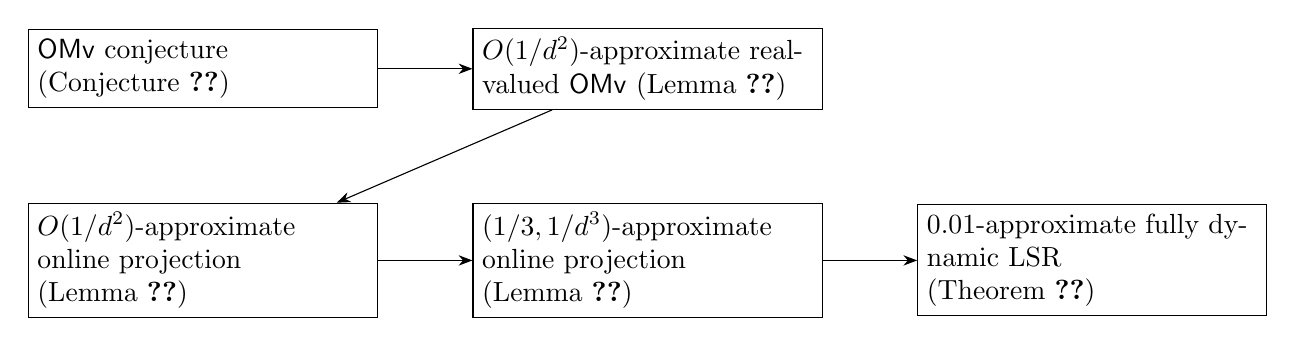
\begin{tikzpicture}[node distance=1.2cm, box/.style={rectangle, draw, text width=4.2cm}, >={Stealth[length=5pt]}]
    % Draw the nodes
    \node[box] (1) {$\omv$ conjecture \\ (Conjecture~\ref{conj:omv})};
    \node[box, right=of 1] (2) {$O(1/d^2)$-approximate real-valued $\omv$ (Lemma~\ref{lem:omv-real})};
    \node[box, below=of 1] (3) {$O(1/d^2)$-approximate online projection (Lemma~\ref{lem:online-projection})};
    \node[box, right=of 3] (4) {$(1/3, 1/d^3)$-approximate online projection (Lemma~\ref{lem:hard-amplification})};
    \node[box, right=of 4] (5) {$0.01$-approximate fully dynamic LSR \\ (Theorem~\ref{thm:lower-full})};

    % Draw the arrows
    \draw[->] (1) -- (2);
    \draw[->] (2) -- (3);
    \draw[->] (3) -- (4);
    \draw[->] (4) -- (5);
  \end{tikzpicture}
  \caption{An illustration of the chain of proofs in this section.}
  \label{fig:fully}
\end{figure}





\subsection{Hardness of online projection}
\label{sec:online-projection}

Recall the definition of the online projection task, which asks to compute the projection of a sequence of online queries $\{\bz^\ttop\}_{t\in [T]}$ onto a fixed subspace $\bU$. 



\Onlineprojection*


For any orthonormal $\bU \in \R^{d\times d_1}$, let $\bU_\perp \in \R^{d\times (d-d_1)}$ be the orthonormal matrix that spans the complementary of the column space of $\bU$, i.e., it satisfies $[\bU, \bU_\perp] \in \R^{d\times d}$ is a squared orthonormal matrix. For any vector $\bz \in \R^d$, define 
\begin{align}
\bz = \bz_{\bU} + \bz_{\bU_\perp} \quad \text{where} \quad \bz_\bU = \bU\bU^{\top}\bz \quad \text{and} \quad \bz_{\bU_\perp} = (\mathbf{I} - \bU\bU^{\top})\bz.
\end{align}
That is to say, $\bz_{\bU}$ is the projection of $\bz$ onto the subspace spanned by the columns of $\bU$, and $\bz_{\bU_{\perp}}$ is the projection of $\bz$ onto the subspace spanned by the complementary of $\bU$. In this section we also denote the projection of a vector $\bz_{k}$ as $\bz_{k, \bU}$.


We prove computing online projection requires $\Omega(d^{2-\gamma})$ amortized time assuming $\omv$.
\begin{lemma}[Hardness of online projection]
\label{lem:online-projection}
Let $\gamma > 0$ be any constant. Assuming the $\omv$ conjecture is true, then there is no algorithm with $\poly(d)$ preprocessing time and $O(d^{2-\gamma})$ amortized running time that can return an $O(1/d^2)$-approximate solution $\hat{\bz}^{\ttop}_{\bU} \in \R^d$ that satisfies $\|\hat{\bz}^{\ttop}_{\bU} - \bU\bU^{\top} \bz^{(t)}\|_2 \leq O(1/d^2)$ for the online projection problem.
\end{lemma}
\begin{proof}
By Lemma \ref{lem:omv-real}, it suffices to reduce from the $O(1/d^2)$-approximate $\omv$ problem of a real-valued PSD matrix $\bH$ with eigenvalues $1/3 \leq \lambda_d(\bH) \leq \cdots \leq \lambda_1(\bH) \leq 1$.
We apply a binary division trick and (approximately) decompose $\bH$ into $k = O(\log d)$ projection matrices $\bU(1), \ldots, \bU(k)$.
Formally, let $\bH = \bU\Sigma \bU^{\top}$ where $\bU \in \R^{d\times d}$ and $\Sigma = \diag(\lambda_1(\bH), \ldots, \lambda_n(\bH))$.
Let $\lambda_{i}(\bH) =0.\lambda_{i,1}\lambda_{i,2}\ldots$ be the binary representation of $\lambda_i$ ($i \in [n]$).
For each $j \in [k]$, let 
\[
S_j = \{i:  i\in [n], \lambda_{i, j} = 1\} \subseteq [n]
\]
be the subset of coordinates with non-zero binary value at the $j$-th bit. Let $\bU(j) = \bU_{*,S_j} \in \R^{d\times |S_j|}$ be an orthonormal matrix that takes columns from $S_j$.





We reduce an $\omv$ instance to $k$ online projection instances, and show that we can compute an $O(1/d^2)$-approximate solution to an $\omv$ query of $\bH$ by using $k$ online projection queries, one for each of the $k$ online projection instances. 
In the preprocessing step, we compute the orthonormal matrices $\bU(1), \ldots, \bU(k)$, and we let them be the initial matrices of the online projection instances. This step can be done in $O(d^3\log d)$ time. 
At the $t$-th step, given an online query $\bz^\ttop \in \R^d$ of $\omv$ with norm $\|\bz^\ttop\|_2 \leq 1$, we make one query for each instance of online projection and let $\bz_j^\ttop$ be the projection returned by the $j$-th instance.
It satisfies 
\begin{align}
\|\bz^{\ttop}_{j} - \bU(j)\bU(j)^{\top}\bz^\ttop\|_2 \leq O(1/d^2). \label{eq:online-proj-guarantee}
\end{align}
The vectors $\bz^\ttop_1, \ldots, \bz^\ttop_k$ can be computed in $k \mathcal{T} = O(\mathcal{T} \cdot \log d)$ (amortized) running time, where $\mathcal{T}$ is the runtime of the online projection algorithm. Finally, we output
\begin{align}
\by^\ttop = \sum_{j=1}^{k} \frac{1}{2^j} \cdot \bz^\ttop_j \label{eq:omv-output}
\end{align}
for the $\omv$ query.
Our goal is to prove $\by^\ttop$ is an $O(1/d^2)$-approximate solution to the $\omv$ query, i.e. 
\begin{align}\label{eq:omv_error}
\|\by^\ttop - \bH\bz^\ttop\|_2 \leq O(1/d^2).
\end{align}

To this end, we have
\begin{align}
\|\by^\ttop - \bH\bz^\ttop\|_2 = &~ \left\|\sum_{j=1}^{k} \frac{1}{2^j} \cdot \bz^\ttop_j - \bH\bz^\ttop\right\|_2 \notag \\
\leq &~  \left\|\sum_{j=1}^{k} \frac{1}{2^j} \cdot \bU(j)\bU(j)^{\top}\bz^\ttop - \bH\bz^\ttop\right\|_2 + \sum_{j=1}^{k}\frac{1}{2^j}\left\|\bU(j)\bU(j)^{\top}\bz^\ttop - \bz_j^\ttop\right\|_2 \notag \\
\leq &~ \left\|\sum_{j=1}^{k} \frac{1}{2^j} \cdot \bU(j)\bU(j)^{\top} \bz^\ttop - \bH\bz^\ttop\right\|_2 + O(1/d^2).\label{eq:online1}
\end{align}
Here the first step follows from the definition of $\by^\ttop$ in Eq.~\eqref{eq:omv-output}, the second step follows from the triangle inequality, and the last step follows from Eq.~\eqref{eq:online-proj-guarantee}.

It remains to bound the first term of RHS, and it suffices to prove $\sum_{j=1}^{k} \frac{1}{2^j} \cdot \bU(j)\bU(j)^{\top}$ is close to $\bH$. 
This holds (almost) by definition. 
Formally, let $\Sigma(j) = \frac{1}{2^j}\diag(\lambda_{1,j}, \ldots, \lambda_{d, j})$ for any $j \geq 1$. By the definition of $\bU(j)$, we have
\begin{align*}
\frac{1}{2^j} \cdot \bU(j)\bU(j)^{\top} =\bU\Sigma(j)\bU^{\top}, \quad \forall j \in [k],
\end{align*}
and therefore 
\begin{align*}
\left\|\bH - \sum_{j=1}^{k}\frac{1}{2^j} \cdot \bU(j)\bU(j)^{\top}\right\|_2 = &~ \left\| \bU \Sigma \bU^{\top} - \sum_{j=1}^{k}\bU\Sigma(j)\bU^{\top}\right\|_2 \\
= &~ \left\|\sum_{j> k} \bU\Sigma(j)\bU^{\top}\right\|_2 \leq \frac{1}{2^{k}} = O(1/d^2),
\end{align*}
where the third step follows from $\| \bU\Sigma(j)\bU^{\top} \|_2 = \frac{1}{2^j} \cdot \|\bU(j) \bU(j)^{\top}\|_2 = \frac{1}{2^j}$, and the last step follows from $k = O(\log d)$.

Plugging into Eq.~\eqref{eq:online1}, we have 
\begin{align*}
\|\by^\ttop - \bH\bz^\ttop\|_2 \leq &~\left\|\sum_{j=1}^{k} \frac{1}{2^j} \cdot \bU(j)\bU(j)^{\top}\bz^\ttop - \bH\bz^\ttop\right\|_2 + O(1/d^2)\\
\leq &~ \left\|\sum_{j=1}^{k} \frac{1}{2^j} \cdot \bU(j)\bU(j)^{\top} - \bH\right\|_2 \|\bz^\ttop\|_2  + O(1/d^2)\\
\leq &~ O(1/d^2)\cdot 1 + O(1/d^2) = O(1/d^2).
\end{align*}


In summary, the above reduction means there exist an $O(1/d^2)$-approximate $\omv$ algorithm for $\bH$ with $O(d^3 \log d)$ preprocessing time and $O(\mathcal{T} \cdot \log d)$ amortized query time. If $\mathcal{T} = O(d^{2-\gamma})$ for some constant $\gamma$, then we can solve the $O(1/d^2)$-approximate $\omv$ problem for $\bH$ in amortized $O(d^{2-\gamma} \cdot \log d)$ time, and by Lemma~\ref{lem:omv-real} this contradicts with the $\omv$ conjecture.
\end{proof}






\subsection{Hardness amplification}
\label{sec:hard-amplification}
So far we have proved an $\Omega(d^{2 - \gamma})$ lower bound of the online projection problem when it is required to output an $O(1/d^2)$-approximate answer per round. 
Our next step is to amplify this approximation precision to a constant.
We first formalize the notion of $(\alpha, \beta)$-approximate projection.

\begin{definition}[$(\alpha, \beta)$-approximate projection]
Given an orthonormal matrix $\bU \in \R^{d\times d_1}$ and a vector $\bz \in \R^{d}$, we say a vector $\by\in \R^{d}$ is an $(\alpha, \beta)$-approximate projection of $\bz$ onto $\bU$, if it satisfies 
\begin{align*}
\|\by - \bU\bU^{\top}\bz\|_2 \leq \alpha \|\bU\bU^\top \bz\|_2 + \beta\|\bz\|_2.
\end{align*}
\end{definition}
As we shall see soon, the interesting regime is $\alpha = \Theta(1)$ and $\beta = 1/\poly(d)$. The problem of online projection (Definition \ref{def:online-projection}) works well with the requirement of outputting an $(\alpha, \beta)$-approximate projection per round. 

\begin{lemma}[Hardness amplification]
\label{lem:hard-amplification}
Let $\gamma > 0$ be any constant. Let $\alpha = 1/3$ and $\beta = O(1/d^3)$.
Assuming the $\omv$ conjecture is true, then there is no algorithm with $\poly(d)$ preprocessing time and $O(d^{2-\gamma})$ amortized running time that can return an $(\alpha, \beta)$-approximate solution for the online projection problem.
\end{lemma}



The reduction is formally shown in Algorithm \ref{algo:hard-amplification}. Our goal is to show that we can answer online projection queries to $O(1/d^2)$ accuracy by using $(\alpha, \beta)$-approximate oracles. We use $\mathbb{P}_\bU, \mathbb{P}_{\bU_\perp}: \R^d \to \R^d$ to denote $(\alpha, \beta)$-approximate projection oracles whose outputs satisfy that for any vector $\bz \in \R^d$, 
(1) $\|\mathbb{P}_{\bU}(\bz) - \bz_\bU\|_2 \leq  \alpha \|\bz_\bU\|_2 + \beta \|\bz\|_2$, and 
(2) $\|\mathbb{P}_{\bU_\perp}(\bz) - \bz_{\bU_\perp}\|_2 \leq  \alpha \|\bz_{\bU_\perp}\|_2 + \beta \|\bz\|_2 $.

The reduction proceeds in $R = \Theta(\log d)$ rounds (i.e., the outer-loop on Line \ref{line:outer}), and we wish to show that each round (1) keeps the projected component $\bz_{r, \bU}$, and (2) reduces the orthogonal component $\bz_{r, \bU_\perp}$ (see Lemma \ref{lem:outer}).
In each round, the reduction first calls the approximate projection oracle onto $\bU_\perp$, which gives a good approximation to the orthogonal component $\bz_{r, \bU_\perp}$, but also has non-negligible component onto space $\bU$.
To resolve this, Algorithm \ref{algo:hard-amplification} proceeds in $K = O(\log d)$ iterations (i.e., inner loop on Line \ref{line:inner}), and in each iteration, it combines the previous output and sends it to $\mathbb{P}_{\bU}$. This process gradually purifies the component onto space $\bU$ (see Lemma \ref{lem:inner-induction}).


\begin{algorithm}[!htbp]
\caption{Hardness amplification}
\label{algo:hard-amplification}
\begin{algorithmic}[1]
\State {\bf Input:} Online query $\bz$, approximate projection oracles $\mathbb{P}_{\bU}$ and $\mathbb{P}_{\bU_\perp}$
\State $\bz_1 \leftarrow \bz$
\For{$r =1,2,\ldots, R$}\Comment{$R = O(\log d)$}\label{line:outer}
\State $\bw_{r, 0} \leftarrow \mathbb{P}_{\bU_\perp}(\bz_r)$
\For{$k=1,2,\ldots, K$}\Comment{$K = O(\log d)$} \label{line:inner}
\State $\by_{r, k} \leftarrow \mathbb{P}_{\bU}(\bw_{r, k-1})$
\State $\bw_{r, k} \leftarrow \bw_{r, k-1} - \by_{r, k} $ \label{line:w-def}
\EndFor
\State $\bz_{r+1} \leftarrow \bz_{r} - \bw_{r, K}$ \label{line:update}
\EndFor
\State \Return $\bz_{R+1}$
\end{algorithmic}
\end{algorithm}



We first state the guarantee of each outer loop. W.l.o.g., we assume $\|\bz\|_2 = 1$.
\begin{lemma}
\label{lem:outer}
For each round $r \in [R]$, we have
\begin{itemize}
\item $\|\bz_{r+1, \bU} - \bz_{r, \bU}\|_2 \leq 4(K+2)\beta$, 
\item $\|\bz_{r+1, \bU_\perp}\|_2 \leq 2\alpha \|\bz_{r, \bU_\perp}\|_2 + 4K^2\beta$, and
\item $\|\bz_{r+1}\|_2 \leq 1 + O(K^4r \beta)$.
\end{itemize}
\end{lemma}


It is useful to first understand the guarantee of the inner loops. 
At the beginning, we have the following lemma for $\bw_{r, 0}$.
\begin{lemma}
\label{lem:inner-begin}
For any round $r \in [R]$, assuming $\|\bz_r\|_2\leq 2$, then we can write 
\begin{align*}
\bw_{r, 0} = \bz_{r, \bU_\perp} - \bdelta_{r, 0} \quad \text{where} \quad \|\bdelta_{r, 0}\|_{2} \leq \alpha \|\bz_{r, \bU_{\perp}}\|_2 + 2\beta.
\end{align*}
\end{lemma}
\begin{proof}
The proof follows directly from the guarantee of $\mathbb{P}_{\bU_\perp}$. In particular, we have that 
\begin{align*}
\|\bw_{r, 0} - \bz_{r, \bU_{\perp}}\|_2 = \|\mathbb{P}_{\bU_\perp}(\bz_r) - \bz_{r, \bU_{\perp}}\|_2 \leq \alpha \|\bz_{r, \bU_{\perp}}\|_2 + \beta \|\bz_r\|_2 \leq \alpha \|\bz_{r, \bU_{\perp}}\|_2 + 2\beta,
\end{align*}
where the second step holds since $\mathbb{P}_{\bU_\perp}$ returns an $(\alpha, \beta)$ approximation over projection onto $\bU_{\perp}$ and the last step holds since $\|\bz_r\|_2 \leq 2$. 
We complete the proof here.
\end{proof}

For each iteration $k \in [K]$, we have the following lemma for the inner loop.
\begin{lemma}
\label{lem:inner-induction}
For any round $r\in [R]$ and iteration $k \in [K]$, assuming $\|\bz_r\|_2 \leq 2$, we can write
\begin{align*}
\bw_{r, k} = \bz_{r, \bU_{\perp}} - (\sum_{\tau = 0}^{k-1} \bdelta_{r, \tau, \bU_{\perp}}) - \bdelta_{r, k}, ~~~\text{and}~~
\by_{r, k} = -\bdelta_{r, k-1, \bU} + \bdelta_{r, k}, 
\end{align*}
and each $\bdelta_{r, k}$ satisfies
\begin{align*}
\|\bdelta_{r, k}\|_2 \leq \alpha \|\bdelta_{r, k-1, \bU}\|_2 + 4 \beta \quad \text{and} \quad \|\bdelta_{r, k}\|_2 \leq \alpha^{k+1}\|\bz_{r, \bU_{\perp}}\|_2 + 4(k+1)\beta.
\end{align*}
\end{lemma}
\begin{proof}
We prove the claim by induction. The base case that $\bw_{r, 0} = \bz_{r, \bU_\perp} - \bdelta_{r, 0}$ and $\|\bdelta_{r, 0}\|_{2} \leq \alpha \|\bz_{r, \bU_{\perp}}\|_2 + 2\beta$ is proved in Lemma~\ref{lem:inner-begin}. (Note that $\by_{r, 0}$ is not defined.)

Suppose the lemma statement holds for $k-1$, which means we have
\begin{align}
\bw_{r, k-1, \bU} = -\bdelta_{r, k - 1, \bU} \label{eq:inner2}
\end{align}
and
\begin{align}
\|\bw_{r, k-1}\|_2 = &~ \left\|\bz_{r, \bU_{\perp}} - (\sum_{\tau=0}^{k-2} \bdelta_{r, \tau, \bU_{\perp}}) - \bdelta_{r, k-1} \right\|_2 \notag \\
\leq &~ \|\bz_{r, \bU_{\perp}}\|_2 + (\sum_{\tau=0}^{k-2} \|\bdelta_{r, \tau, \bU_{\perp}}\|_2) + \|\bdelta_{r, k-1}\|_2 \notag \\
\leq &~ \|\bz_{r, \bU_{\perp}}\|_2 + \sum_{\tau=0}^{k-1} \|\bdelta_{r, \tau}\|_2  \notag\\
\leq &~ \sum_{\tau=0}^{k} \Big( \alpha^{\tau}\|\bz_{r, \bU_{\perp}}\|_2 + 4(\tau+1)\beta \Big) \notag \\
\leq &~ \frac{1-\alpha^{k+1}}{1-\alpha} \cdot \|\bz_{r, \bU_{\perp}}\|_2 + 4K^2\beta \leq 4, \label{eq:inner3}
\end{align}
where the second step holds from triangle inequality, the third step follows from 
\[
\|\bdelta_{r, \tau}\|_2^2 = \|\bdelta_{r, \tau, \bU} + \bdelta_{r, \tau, \bU_\perp}\|_2^2 = \|\bdelta_{r, \tau, \bU}\|_2^2 + \|\bdelta_{r, \tau, \bU_\perp}\|_2^2 \geq \|\bdelta_{r, \tau, \bU}\|_2^2,
\]
the fourth step holds from Lemma \ref{lem:inner-begin} and the induction hypothesis.
The last step follows the choice of $\alpha = 1/3, \beta = O(1/d^3)$, $K = O(\log d)$, and $\|\bz_{r, \bU_\perp}\|_2 \leq \|\bz_{r}\|_2 \leq 2$.

Now we are ready to prove that the induction hypothesis also holds for the $k$-th iteration.

{\bf Properties of $\bdelta_{r,k}$ and $\by_{r,k}$.}
We have
\begin{align}
\|\by_{r, k} + \bdelta_{r, k-1, \bU}\|_2 = &~ \|\mathbb{P}_{\bU}(\bw_{r, k-1}) + \bdelta_{r, k-1, \bU}\|_2 = \|\mathbb{P}_{\bU}(\bw_{r, k}) -  \bw_{r, k-1, \bU}\|_2\notag \\
\leq &~ \alpha\|\bw_{r, k-1, \bU}\|_2 + \beta \|\bw_{r, k-1}\|_2 = \alpha\|\bdelta_{r, k-1, \bU}\|_2 + 4\beta, \label{eq:inner4}
\end{align}
where the first step follows from the definition that $\by_{r, k} = \mathbb{P}_{\bU}(\bw_{r, k-1})$, the second step follows from Eq.~\eqref{eq:inner2}, the third step holds from the guarantee of $\mathbb{P}_{\bU}$ and the last step holds from Eq.~\eqref{eq:inner2}\eqref{eq:inner3}. 

Hence, define $\bdelta_{r, k} = \by_{r, k} + \bdelta_{r, k-1, \bU}$, from Eq.~\eqref{eq:inner4} we have that
\begin{align*}
\|\bdelta_{r, k}\|_2 \leq \alpha \|\bdelta_{r, k-1, \bU}\|_2 + 4\beta.
\end{align*}
Note that this definition of $\bdelta_{r, k}$ also gives us that
\begin{equation}\label{eq:inner_y}
\by_{r, k} = \bdelta_{r, k} - \bdelta_{r, k-1, \bU}.
\end{equation}
By induction hypothesis, we also have 
\[
\|\bdelta_{r, k}\|_2 \leq \alpha \|\bdelta_{r, k-1, \bU}\|_2 + 4\beta \leq \alpha\|\bdelta_{r, k-1}\|_2 + 4\beta \leq \alpha^{k + 1}\|\bz_{r, \bU_{\perp}}\|_2 + 4(k+1)\beta.
\]

{\bf Property of $\bw_{r,k}$.} We have
\begin{align*}
\bw_{r, k} = &~ \bw_{r, k-1} - \by_{r,k} \\
= &~ \Big( \bz_{r, \bU_{\perp}} - (\sum_{\tau=0}^{k-2} \bdelta_{r, \tau, \bU_{\perp}}) - \bdelta_{r, k-1}\Big) - \Big( \bdelta_{r, k} - \bdelta_{r, k-1, \bU} \Big)\\
= &~ \bz_{r, \bU_{\perp}} - (\sum_{\tau=0}^{k-1} \bdelta_{r, \tau, \bU_{\perp}}) - \bdelta_{r, k}.
\end{align*}
Here the first step follows from the definition of $\bw_{r, k}$ (Line \ref{line:w-def}), the second step follows from the induction hypothesis about $\bw_{r,k-1}$ and Eq.~\eqref{eq:inner_y} that we just proved. We conclude the proof here.
\end{proof}


Now we can go back to analyse the outer loops and prove Lemma \ref{lem:outer}.
\begin{proof}[Proof of Lemma \ref{lem:outer}]
Consider any round $r \in [R]$. We have
\begin{align}
\bz_{r+1} = &~ \bz_{r} - \bw_{r, K} \notag \\
= &~ \bz_{r} - \Big( \bz_{r, \bU_{\perp}} - (\sum_{\tau = 0}^{K-1} \bdelta_{r, \tau, \bU_{\perp}}) - \bdelta_{r, K} \Big) \notag \\
= &~ \bz_{r, \bU} + (\sum_{\tau = 0}^{K-1} \bdelta_{r, \tau, \bU_{\perp}}) + \bdelta_{r, K} \label{eq:outer1}
\end{align}
Here the first step follows from the update rule (Line \ref{line:update}), the second step follows from Lemma \ref{lem:inner-induction}. 

Hence, we have $\bz_{r+1, \bU} = \bz_{r, \bU} + \bdelta_{r, K, \bU}$, so for the first claim, we have
\begin{align*}
\|\bz_{r+1, \bU} - \bz_{r, \bU}\|_2 = &~ \|\bdelta_{r, K, \bU}\|_2 \leq \|\bdelta_{r, K}\|_2\\
\leq &~ \alpha^{K+1}\|\bz_{r, \bU_\perp}\|_2 + 4(K+1)\beta \leq 4(K+2)\beta.
\end{align*}
Here the third step follows from Lemma \ref{lem:inner-induction}, the last step follows from $\|\bz_{r, \bU_\perp}\|_2 \leq \|\bz_{r}\|_2 \leq 2$, and the choice of parameter that $K = O(\log d)$, $\alpha = 1/3$ and $\beta = O(1/d^3)$, so that $\alpha^K < \beta$.


For the second claim, the orthogonal component $\bz_{r+1, \bU_\perp}$ satisfies
\begin{align*}
\|\bz_{r+1, \bU_\perp}\|_2 = &~ \left\|\sum_{k=0}^{K} \bdelta_{r, k, \bU_\perp}\right\|_2 \leq \sum_{k=0}^{K}\|\bdelta_{r, k, \bU_\perp}\|_2 \leq \sum_{k=0}^{K}\|\bdelta_{r, k}\|_2 \\
\leq &~ \sum_{k=0}^{K} \Big( \alpha^{k+1}\|\bz_{r, \bU_\perp}\|_2 + 4(k+1) \beta \Big) \\
\leq &~ 2\alpha \|\bz_{r, \bU_\perp}\|_2 + 4K^2 \beta,
\end{align*}
where the first step follows from Eq.~\eqref{eq:outer1}, the second step follows from triangle inequality, the fourth step follows from Lemma \ref{lem:inner-induction}, and the last step follows from the choice of parameter that $\alpha = 1/3$.


Finally, we prove the third claim by induction on $r$. First note that in the base case where $r=0$, by definition we have $\bz_{1, \bU} = \bz$, so $\|\bz_{1, \bU}\|_2 = \|\bz\|_2 = 1$. Suppose the third claim continues to hold up to round $r-1$, for the $r$-th round, we have
\begin{align*}
\|\bz_{r+1}\|_2^2 = &~ \|\bz_{r+1, \bU_\perp}\|_2^2 + \|\bz_{r+1, \bU}\|_2^2 \\
\leq &~ \big(2\alpha \|\bz_{r, \bU_\perp}\|_2 + 4K^2\beta \big)^2 + \big(\|\bz_{r, \bU}\|_2 + 4(K+2)\beta \big)^2 \\
\leq &~ \big(\|\bz_{r, \bU_\perp}\|_2 + 4K^2\beta \big)^2 + \big(\|\bz_{r, \bU}\|_2 + 4 K^2 \beta \big)^2 \\
= &~ (\|\bz_{r, \bU_\perp}\|_2^2 + \|\bz_{r, \bU}\|_2^2) + 8 K^2 \beta \cdot (\|\bz_{r, \bU_\perp}\|_2 + \|\bz_{r, \bU}\|_2) + 32 K^4 \beta^2 \\
\leq &~ \|\bz_r\|_2^2 + 16 K^2 \beta \cdot \|\bz_r\|_2 + 32 K^4 \beta^2 \\
\leq &~ 1 + O(K^4 r \beta),
\end{align*}
where the second step follows from the first two claims that we just proved: $\|\bz_{r+1, \bU_\perp}\|_2 \leq 2\alpha \|\bz_{r, \bU_\perp}\|_2 + 4K^2\beta$, and $\|\bz_{r+1, \bU}\|_2 \leq \|\bz_{r, \bU}\|_2 + \|\bz_{r+1, \bU} - \bz_{r, \bU}\|_2 \leq \|\bz_{r, \bU}\|_2 + 4(K+2)\beta$, the third step follows from $2 \alpha < 1$ since $\alpha = 1/3$ and $K+2 < K^2$ since $K = O(\log d)$, the fifth step follows from $\|\bz_r\|_2^2 = \|\bz_{r, \bU_\perp}\|_2^2 + \|\bz_{r, \bU}\|_2^2$, and the last step follows from the induction hypothesis that $\|\bz_r\|_2 \leq 1 + O(K^4 (r-1) \beta)$, and that $K^2 \beta < K^4 \beta$ and $K^4 \beta^2 < K^4 \beta$.
\end{proof}



Now we can wrap up the reduction and prove Lemma \ref{lem:hard-amplification}.
\begin{proof}[Proof of Lemma \ref{lem:hard-amplification}]
We prove that if there is an algorithm that outputs $(\alpha, \beta)$-approximate solutions for the online projection problem in $O(d^{2-\gamma})$ amortized time, then we can use this algorithm to obtain $O(1/d^2)$-approximate solutions for the online projection problem in $O(d^{2-\gamma + o(1)})$ amortized time, and hence contradicts with Lemma~\ref{lem:online-projection}.

Given an orthonormal matrix $\bU$ and let $\bz^\ttop$ be the query at the $t$-th round of the online projection problem, then we perform the reduction shown in Algorithm \ref{algo:reduction} and its output $\bz^\ttop_{R+1}$ satisfies
\begin{align*}
\|\bz_{R+1, \bU}^\ttop - \bz_{\bU}^\ttop\|_2 = &~ \|\bz_{R+1, \bU}^\ttop - \bz_{1, \bU}^\ttop\|_2 \leq \sum_{r=1}^{R} \|\bz_{r+1, \bU}^\ttop - \bz_{r, \bU}^\ttop\|_2 \leq O(RK\beta).
\end{align*}
Here the first inequality follows from triangle inequality and the second one holds due to the first claim of Lemma \ref{lem:outer}.
Meanwhile, due to the second claim of Lemma \ref{lem:outer}, we have
\begin{align*}
\|\bz_{R+1, \bU_\perp}^\ttop\|_2 \leq (2\alpha)^{K}\|\bz_{1, \bU_\perp}^\ttop\|_2 + O(RK^2\beta) \leq O(RK^2\beta),
\end{align*}
where the second step follows from that $(2 \alpha)^K < 1/d^3$ since $K = O(\log d)$ and $\alpha = 1/3$.

Combining the above two inequalities, and since $R = O(\log d)$, $K = O(\log d)$, and $\beta = O(1/d^3)$, we obtain
\begin{align*}
\|\bz_{R+1}^\ttop - \bz_{\bU}^\ttop\|_2 \leq \|\bz_{R+1, \bU}^\ttop - \bz_{\bU}^\ttop\|_2 + \|\bz_{R+1, \bU_\perp}^\ttop\|_2 \leq O(RK\beta  + RK^2\beta) \leq O(1/d^2).
\end{align*}
That is to say, $\bz_{R+1}^\ttop$ is an $O(1/d^2)$-approximate projection of $\bz^\ttop$ onto $\bU$.


We still need to bound the runtime of the reduction. Let $\mathcal{T}$ denote the amortized query time of the $(\alpha, \beta)$-approximate oracles $\mathbb{P}_{\bU_\perp}$ and $\mathbb{P}_{\bU}$. The reduction involves $R = O(\log d)$ outer loops, with each outer loop requiring a single call to $\mathbb{P}_{\bU_\perp}$ and containing $K = O(\log d)$ inner loops. During each inner loop, a single call to $\mathbb{P}_{\bU}$ is made, and the construction of $\bw_{r,k}$ takes $O(d)$ time.

Therefore, we can conclude that the total runtime of the algorithm is bounded by $RK \cdot \mathcal{T} + O(RKd) = (\mathcal{T} + d) \cdot O(\log^2 d)$. If $\mathcal{T} = O(d^{2-\gamma})$, then we can solve the $O(1/d^2)$-approximate online projection problem in amortized $O(d^{2-\gamma} \cdot \log^2 d)$ time, and this contradicts with the $\omv$ conjecture by Lemma~\ref{lem:online-projection}. This completes the proof.
\end{proof}




As a corollary, we prove the hardness of constant approximate-$\omv$.
\begin{theorem}[Hardness of approximate-$\omv$]
\label{thm:hard-omv-approx}
Let $d$ be a sufficiently large integer and $T = \poly(d)$.
Let $\gamma > 0$ be any constant, $\alpha = 1/3$ and $\beta = O(1/d^3)$. 
Let $\bH\in \R^{d\times d}$ ($\|\bH\|_2 =1$), and $\bz^{(1)}, \ldots, \bz^{(T)}$ be online queries ($\|\bz^\ttop\|_2 = 1$).
Assuming the $\omv$ conjecture is true, then there is no algorithm with $\poly(d)$ preprocessing time and $O(d^{2-\gamma})$ amortized running time that can return an $(\alpha, \beta)$-approximate answer to $\bH\bz^\ttop$ for all $t \in [T]$, i.e., a vector $\by^\ttop$ s.t. $\|\by^\ttop - \bH\bz^\ttop\|_2 \leq \alpha \|\bH\bz^\ttop\|_2 + \beta$. This continues to hold when $\bH$ is a projection matrix.
\end{theorem}




















\subsection{Reduction from online projection to fully dynamic LSR}
\label{sec:reduction}
Finally, we provide a reduction from $(\alpha, \beta)$-approximate online projection to $\epsilon$-approximate fully dynamic LSR, where $\alpha = 1/3$, $\beta = O(1/d^3)$, and $\eps = \frac{1}{100}$. 
Given an instance of online projection with orthonormal matrix $\bU \in \R^{d \times d_1}$, we first set up the LSR problem.

\vspace{+2mm}
{\bf \noindent Setup for reduction \ \ } Let 
\begin{align*}
\bA^{(0)} = 
\left[
\begin{matrix}
\sqrt{\lambda} \cdot \mathbf{I}_d \\
(\bU_\perp)^{\top}
\end{matrix}
\right] \in \R^{(2d-d_1) \times d}  \quad \text{and} \quad \bb^{(0)} = 
\left[
\begin{matrix}
\mathbf{0}_d\\
\frac{1}{\sqrt{d}} \cdot \mathbf{1}_{d-d_1}
\end{matrix} 
\right] 
\in \R^{2d-d_1}
\end{align*}
where $\lambda = 1/d^{40}$. For convenience, we have included a notation table in Table~\ref{tab:parameters}.


\begin{table}[ht]
\centering
\begin{tabular}{|c|c|c|}
\hline
Parameter & Value & Comment \\ \hline
$\eps$ & $< 1/100$ & approximation factor of fully dynamic LSR \\ \hline
$\lambda$ & $1/d^{40}$ & coefficient of the regularization term \\ \hline
$\alpha$ & $1/3$ & approximation factor of online projection \\ \hline
\end{tabular}
\caption{Parameters used in the reduction from online projection to fully dynamic LSR}
\label{tab:parameters}
\end{table}

It would be convenient to view the first $d$ rows as a regularization term, and the (squared) loss equals to
\begin{align*}
L(\bx) := \|\bA^{(0)} \bx - \bb^{(0)}\|_2^2 = \left\|(\bU_\perp)^{\top}\bx - \frac{1}{\sqrt{d}} \cdot \mathbf{1}_{d-d_1}\right\|_2^2 + \lambda \|\bx\|_2^2.
\end{align*}
In the processing step, we also compute
\begin{equation}\label{eq:def_x*}
\bx^{*} := \frac{1}{\sqrt{d}} \sum_{j=1}^{d-d_1}\bU_{\perp,j} \in \R^d,
\end{equation}
where with a slight abuse of notation we let $\bU_{\perp, j} \in \R^d$ denote the $j$-th column of matrix $\bU_\perp$ (Hence $\bx^{*}$ also lies in the column space of $\bU_\perp$).
Overall, the preprocessing step takes at most $O(d^\omega)$ time. 


\vspace{+2mm}
{\bf \noindent Online projection query \ \ } Given an online projection query $\bz^\ttop \in \R^{d}$ of the $t$-th step, recall our goal is to find an $(\alpha, 1/d^3)$-approximate projection onto $\bU$.

The reduction is formally presented in Algorithm \ref{algo:reduction}. First, it inserts a new row of $(\frac{1}{10}\cdot \bz^\ttop, 1)$ to the matrix, and then it calls the dynamic LSR solver (Line \ref{line:regression}) to obtain an $\eps$-approximate solution $\bx^\ttop$. The final output is determined as follows: if the component $\bz_\bU^\ttop$ is already sufficiently small, then it is captured by the condition on Line \ref{line:termination}, and we can simply output $\bf{0}$. Otherwise, Algorithm \ref{algo:reduction} outputs a scaled version of $(\bx^\ttop - \bx^{*})$, where the scaling factor is determined by Eq.~\eqref{eq:interpolation}. Finally, the new row is deleted, and we return to the original setup.


\begin{algorithm}[!htbp]
\caption{Reduction: From $(\alpha, 1/d^3)$-approximate online projection to $\epsilon$-approximate dynamic LSR}
\label{algo:reduction}
\begin{algorithmic}[1]
\State Insert $(\frac{1}{10}\cdot\bz^\ttop, 1) \in \R^{d}\times \R$ \Comment{Insert a new row}
\State Call the regression solver and let $\bx^{\ttop}$ be an $\eps$-approximate solution of the square root of \label{line:regression}
\begin{align}
L^\ttop(\bx) := \left\|(\bU_{\perp})^\top\bx - \frac{1}{\sqrt{d}} \cdot \mathbf{1}_{d-d_1}\right\|_2^2 + \frac{1}{100}|\langle \bz^\ttop, \bx\rangle - 10|^2 + \lambda \|\bx\|_2^2   \label{eq:lsr-r}
\end{align}
\State $\by^\ttop \leftarrow \bx^{\ttop} - \bx^{*}$ \label{line:y-rt}
\If{$\|\by^\ttop\|_2 \geq d^3$ \textbf{or} $|10 - \langle \bz^\ttop, \bx^\ttop\rangle| \geq 200 d^4\sqrt{\lambda}$}  
\label{line:termination}
\State \Return $\hat{\bz}_\bU^\ttop \leftarrow \mathbf{0}$ 
\Else
\State \Return $\hat{\bz}_\bU^\ttop \leftarrow \xi^{*} \cdot \by^\ttop$ where \label{line:interpolation}
\begin{align}
\xi^{*} = \arg\min_{\xi} \|\bz^\ttop - \xi \cdot \by^\ttop\|_2 \label{eq:interpolation}
\end{align}
\EndIf
\State Delete the row $(\frac{1}{10}\cdot\bz^\ttop, 1)$ \Comment{Delete the new row}
\end{algorithmic}
\end{algorithm}

Intuitively, the first term $\|(\bU_{\perp})^\top\bx - \frac{1}{\sqrt{d}} \cdot \mathbf{1}_{d-d_1}\|_2^2$ of the loss $L^\ttop(\bx)$ enforces the approximate solution $\bx^{(t)}$ to satisfy that $\bx^{(t)}_{\bU_{\perp}} \approx \bx^*$ on the subspace $\bU_{\perp}$, since $\bx^*$ is the minimizer of the first term. The second term $\frac{1}{100}|\langle \bz^\ttop, \bx\rangle - 10|^2$ then enforces $\bx^{(t)}_{\bU}$ to be close to a scaled version of $\bz^{(t)}_{\bU}$. Thus, $(\bx^{(t)} - \bx^*)$ is approximately a scaled version of $\bz^{(t)}_\bU$.




Formally, our goal is to prove the following lemma.
\begin{lemma}
\label{lem:reduction-lsr}
For any $t \in [T]$, the output of Algorithm \ref{algo:reduction} satisfies
\begin{align*}
\|\hat{\bz}_{\bU}^{\ttop} - \bz_{\bU}^\ttop\|_2 \leq \alpha \|\bz_\bU^\ttop\|_2 + O(1/d^3).
\end{align*}
\end{lemma}
\begin{proof}
We will prove the lemma by considering three different cases. We first give a short summary.
\begin{itemize}
\item {\bf Case 1: $\|\bz_{\bU}^\ttop\|_2 \geq 1/d^4$.} We prove that in this case we always have $|10 - \langle \bz^\ttop, \bx^{(t)}\rangle| \geq 200 d^4\sqrt{\lambda}$, so the condition of Line~\ref{line:termination} reduces to test whether $\|\by^\ttop\|_2 \geq d^3$ or not.
\begin{itemize}
\item {\bf Case 1-1: $\|\by^\ttop\|_2 \geq d^3$.} Then the condition of Line \ref{line:termination} is satisfied and we prove $\|\bz_\bU^\ttop\|_2 \leq 1/d^3$, so it is fine to output $\hat{\bz}_\bU^\ttop = \bf{0}$.
\item {\bf Case 1-2: $\|\by^\ttop\|_2 < d^3$.} Then the condition is not satisfied, and we prove the output $\hat{\bz}_\bU^\ttop = \xi^{*} \cdot \by^\ttop$ is an $(\alpha, 1/d^3)$-approximate projection of $\bz^\ttop$. 
This is the main technical part of the proof.
\end{itemize}
\item {\bf Case 2: $\|\bz_{\bU}^\ttop\|_2 < 1/d^4$.} In this case we prove that the termination condition of Line \ref{line:termination} must be true, and therefore, the output $\bz^{\ttop} = \mathbf{0}$ is an $O(1/d^3)$-approximation of $\bz_\bU^{\ttop}$.
\end{itemize}
Before going into details of the three cases, we first define a vector
\begin{align}\label{eq:x_rt*}
\bx^{*}_{t} = \bx^{*} + \frac{10 - \langle \bz_{\bU_\perp}^\ttop,\bx^{*}\rangle}{\|\bz_{\bU}^\ttop\|_2^2} \bz_{\bU}^\ttop \in \R^d.
\end{align}
We note $\bx^{*}_{t}$ is not the optimal solution of Eq.~\eqref{eq:lsr-r}, but it gives a good upper bound of the loss. 

To understand the role of $\bx_t^{*}$, note that if $\bx^{*}_{t}$ is a good approximation of the optimal solution of Eq.~\eqref{eq:lsr-r}, then $\bx^{\ttop}$ will be close to $\bx^{*}_{t}$, so $\by^\ttop = \bx^{\ttop} - \bx^{*} \approx \bx^{*}_{t} - \bx^{*}$. As a result, $\|\by^\ttop\|_2 \approx \|\bx^{*}_{t} - \bx^{*}\|_2 = O(1/\|\bz_\bU^\ttop\|_2)$. If $\|\by^\ttop\|_2 \geq d^3$ (the first part of the termination condition on Line~\ref{line:termination}) then we have $\|\bz_{\bU}^\ttop\|_2$ is small, so $\mathbf{0}$ is a good approximation of $\bz^{\ttop}_{\bU}$. 
On the other hand, if $\bx^{*}_{t}$ is not a good approximation of the optimal solution of Eq.~\eqref{eq:lsr-r}, then this means $\|\bz_{\bU}^\ttop\|_2$ is way too small, and we can capture this by the second part of the termination condition, i.e., the second term in the objective will be large.

One can verify that $\bx^{*}_{t}$ obtains zero loss except for the third regularization term. That is, it satisfies 
\begin{align*}
\langle \bx^{*}_{t}, \bU_{\perp, j}\rangle = &~ \langle \bx^{*}, \bU_{\perp,j}\rangle = \frac{1}{\sqrt{d}}, \quad \forall j \in [d-d_1], \\
\text{and, } \langle \bx^{*}_{t}, \bz^\ttop\rangle = &~\langle \bx^{*}, \bz_{\bU_\perp}^\ttop \rangle + \frac{10 - \langle \bz_{\bU_\perp}^\ttop,\bx^{*}\rangle}{\|\bz_{\bU}^\ttop\|_2^2}\cdot \langle \bz_{\bU}^\ttop, \bz_{\bU}^\ttop\rangle = 10,
\end{align*}
where the first step of the second equation follows from $\bx^*$ is in the subspace $\bU_\perp$ so it's orthogonal to $\bz_{\bU}^\ttop$.
Consequently, we have $\|(\bU_\perp)^{\top}\bx_{t}^{*} - \frac{1}{\sqrt{d}} \cdot \mathbf{1}_{d-d_1}\|_2 = 0$ and $|\langle \bz^\ttop, \bx_{t}^{*}\rangle - 10| = 0$, so $L^\ttop(\bx_{t}^{*})$ defined in Eq.~\eqref{eq:lsr-r} satisfies
\begin{align}
L^\ttop(\bx_{t}^{*}) = \lambda\|\bx_{t}^{*}\|_2^2 
\leq \lambda \cdot \frac{(10 - \langle \bz_{\bU_\perp}^\ttop,\bx^{*}\rangle)^2}{\|\bz_{\bU}^\ttop\|_2^2} + \lambda := \lambda (\Delta_{t}^2 + 1),
\label{eq:loss}
\end{align}
Here the second step follows from the definition of $\bx_{t}^{*}$ in Eq.~\eqref{eq:x_rt*}, and that $\bx^*$ has norm $\|\bx^*\|_2 \leq 1$ and it's orthogonal to $\bz_{\bU}^\ttop$, for notational convenience in the third step we have defined
\begin{equation}\label{eq:def_Delta_rt}
\Delta_{t} := \frac{10 - \langle \bz_{\bU_\perp}^\ttop, \bx^{*}\rangle}{\|\bz_{\bU}^\ttop\|_2}.
\end{equation}


\vspace{+2mm}
{\bf \noindent Case 1 \ \ } Suppose $\|\bz_{\bU}^\ttop\|_2 \geq 1/d^4$. Since $\|\bx^{*}\|_2 \leq 1$ and $\|\bz_{\bU}^\ttop\|_2 \leq 1$, we have 
\begin{align}\label{eq:Delta_bound}
\Delta_{t} = \frac{10 - \langle \bz_{\bU_\perp}^\ttop, \bx^{*}\rangle}{\|\bz_{\bU}^\ttop\|_2} \in (9,  11d^4].
\end{align}
Therefore by Eq.~\eqref{eq:loss} we have
\begin{align*}
L^\ttop(\bx_{t}^{*}) \leq \lambda (\Delta_{t}^2 + 1) \leq \lambda \cdot (1 + 121d^8).
\end{align*}
The solution $\bx^\ttop$ is $\eps$-approximately optimal where $\eps \leq 1/100$, so
\begin{align}
L^\ttop(\bx^\ttop) \leq (1+\eps)^2 \cdot L^\ttop(\bx_{t}^*) \leq 200\lambda d^8. \label{eq:loss2}
\end{align} 
This implies that
\[
\frac{1}{100} |10 - \langle \bz^\ttop, \bx^{(t)}\rangle|^2 \leq L^\ttop(\bx^{(t)}) \leq 200 \lambda d^8.
\]
So in this case we always have $|10 - \langle \bz^\ttop, \bx^{(t)}\rangle| < 200 d^4\sqrt{\lambda}$, and this means the termination condition on Line~\ref{line:termination} is equivalent to whether $\|\by^\ttop\|_2 \geq d^3$.


We make the following claim about $\bx^\ttop$, and we defer the proof of this claim to Appendix \ref{sec:fully-app}, as it involves some detailed calculations.
\begin{claim}
\label{claim:decomposition}
Let $\bV_{t}$ be the orthonormal matrix that concatenates $\bU_\perp$ and $\bz_{\bU}^\ttop$, i.e, $\bV_{t} := [\bU_\perp, \frac{\bz_{\bU}^\ttop}{\|\bz_{\bU}^\ttop\|_2}]$. Then we have
\begin{align*}
\bU_\perp(\bU_\perp)^{\top} \bx^\ttop = &~  \bx^{*} \pm 20d^4 \sqrt{\lambda}, \\
\langle \bx^\ttop, \bz_{\bU}^\ttop\rangle = &~  10 - \langle \bz_{\bU_\perp}^\ttop,\bx^{*}\rangle \pm 200d^4 \sqrt{\lambda}, \\
\|(\mathbf{I} - \bV_{t}\bV_{t}^{\top}) \cdot \bx^\ttop\|_2 \leq &~ 2\sqrt{\eps} \cdot \Delta_{t}.
\end{align*}
\end{claim}



Using Claim \ref{claim:decomposition}, we can write $\bx^\ttop$ as
\begin{align*}
\bx^\ttop = &~ \bU_\perp (\bU_\perp)^{\top} \bx^\ttop + \frac{\langle \bx^\ttop, \bz^\ttop_{\bU} \rangle}{\|\bz^\ttop_{\bU}\|_2} \cdot \frac{\bz^\ttop_{\bU}}{\|\bz_{\bU}^\ttop\|_2} + \bz_{\perp\perp}^\ttop \\
= &~ \bx^{*} + \Delta_{t}\cdot  \frac{\bz^\ttop_{\bU}}{\|\bz_{\bU}^\ttop\|_2} + \bz_{\perp\perp}^\ttop \pm O(d^8\sqrt{\lambda}),
\end{align*}
where the first step follows from decomposing $\bx_r^\ttop$ into three parts: the component that is in subspace $\bU_\perp$, the component that is in the same direction as $\bz_{\bU}^\ttop$, and the component that is orthogonal to both $\bU_\perp$ and $\bz^\ttop_{\bU}$ which we denote as $\bz_{\perp\perp}^\ttop := (\mathbf{I} - \bV_{t}\bV_{t}^{\top}) \cdot \bx^\ttop$, the second step follows from the first and second parts of Claim~\ref{claim:decomposition} and that $\|\bz_{\bU}^\ttop\|_2 \geq 1/d^4$, and finally note that using the third part of Claim~\ref{claim:decomposition} we have 
\begin{equation}\label{eq:z_perp_perp_bound}
\|\bz_{\perp\perp}^\ttop\|_2 \leq 2\sqrt{\eps}\cdot \Delta_{t}.
\end{equation}


Consequently, we can write $\by^\ttop$ as
\begin{align}\label{eq:y_rt}
    \by^\ttop = \bx^\ttop - \bx^* = \Delta_{t}\cdot  \frac{\bz^\ttop_{\bU}}{\|\bz_{\bU}^\ttop\|_2} + \bz_{\perp\perp}^\ttop \pm O(d^8\sqrt{\lambda}).
\end{align}

We further divide into two cases based on whether $\|\by^\ttop\|_2 \geq d^3$, i.e., whether the termination condition is satisfied.

\vspace{+2mm}
{\bf \noindent Case 1-1 \ \ } Suppose $\|\by^\ttop\|_2 \geq d^3$. Then it meets the termination condition and we return $\hat{\bz}_{U}^\ttop = \mathbf{0}$. 
In this case, we have
\begin{align*}
d^3 \leq \|\by^\ttop\|_2 = &~ \left\|\Delta_{t}\cdot  \frac{\bz^\ttop_{\bU}}{\|\bz_{ \bU}^\ttop\|_2} + \bz_{\perp\perp}^\ttop\right\|_2  \pm O(d^8\sqrt{\lambda} ) \\
\leq &~\Delta_{t} + \|\bz_{\perp\perp}^\ttop\|_2 \pm O(d^8\sqrt{\lambda} ) \leq (1+2\sqrt{\eps})\Delta_{t}  \pm O(d^8\sqrt{\lambda} ),
\end{align*}
where third step follows from triangle inequality, and the last step follows from Eq.~\eqref{eq:z_perp_perp_bound}. 
Since $\lambda = 1/d^{40}$ and $\eps = 1/100$, we conclude that
\begin{align*}
\frac{1}{2}d^3 \leq \Delta_{t} =  \frac{10 - \langle \bz_{\bU_\perp}^\ttop,\bx^{*}\rangle}{\|\bz_{ \bU}^{(t)}\|_2}
\leq \frac{11}{\|\bz_{\bU}^{(t)}\|_2},
\end{align*}
and therefore, $\|\bz_{\bU}^\ttop\|_2 \leq O(1/d^3)$ and it is fine to return $\hat{\bz}_{\bU}^\ttop = \mathbf{0}$.


\vspace{+2mm}
{\bf \noindent Case 1-2 \ \ } 
Suppose $\|\by^\ttop\|_2 < d^3$. Then the termination condition is not met. 
To compute $\hat{\bz}_\bU^\ttop$, we need to solve Eq.~\eqref{eq:interpolation}. Define $\xi  = \Delta_{t}^{-1} \cdot \|\bz_{\bU}^\ttop\|_2$, and we have
\begin{align}
\|\bz^\ttop - \xi \by^\ttop\|_2^2 = &~ \Big\|\bz_{\bU_\perp}^\ttop - \Delta_{t}^{-1} \cdot \|\bz_{\bU}^\ttop\|_2 \cdot \big( \bz_{\perp\perp}^\ttop \pm O(d^{8}\sqrt{\lambda}) \big) \Big\|_2^2\notag \\
= &~ \|\bz_{\bU_\perp}^\ttop\|_2^2 + \Delta_{t}^{-2} \cdot \|\bz_{\bU}^\ttop\|_2^2 \cdot \|\bz_{\perp\perp}^\ttop\|_2^2 \pm O(d^{8}\sqrt{\lambda}) \label{eq:ub1}.
\end{align}
The first step follows from Eq.~\eqref{eq:y_rt} and $\bz^\ttop = \bz_{\bU}^\ttop + \bz_{ \bU_{\perp}}^\ttop$, the second step holds since $\bz_{\bU_\perp}^\ttop$ is orthogonal to $\bz_{ \perp\perp}^\ttop$, and the error term is still $\pm O(d^8 \sqrt{\lambda})$ since $\|\bz_{\bU}^\ttop\|_2, \|\bz_{\bU_{\perp}}^\ttop\|_2, \|\bz_{\perp\perp}^\ttop\|_2 \leq 1$ and $\Delta_{t} \geq 9$ (Eq.~\eqref{eq:Delta_bound}). 


The optimal solution to Eq.~\eqref{eq:interpolation}, denoted as $\xi^{*}$, can be expressed as $\xi^{*} = (1 + \nu)\Delta_t^{-1} \|\bz_\bU^\ttop\|_2$ for some scaling factor $\nu$. Similarly, we have
\begin{align}
\|\bz^\ttop - \xi^{*}\by^\ttop\|_2^2 = &~ \Big\|\bz_{\bU}^\ttop + \bz_{\bU_\perp}^\ttop - (1 + \nu)\Delta_t^{-1}\|\bz_\bU^\ttop\|_2 \cdot \Big(\Delta_{t}\cdot  \frac{\bz^\ttop_{\bU}}{\|\bz_{\bU}^\ttop\|_2} + \bz_{\perp\perp}^\ttop\Big)   \Big\|_2^2 \pm O(d^8\sqrt{\lambda}) \notag \\
= &~ \|\bz_{\bU_\perp}^\ttop\|_2^2 + \nu^2 \|\bz_{\bU}^\ttop\|_2^2 + (1+\nu)^2 \Delta_{t}^{-2} \cdot \|\bz_{\bU}^\ttop\|_2^2 \cdot \|\bz_{\perp\perp}^\ttop\|_2^2 \pm O(d^{8}\sqrt{\lambda}),\label{eq:ub2}
\end{align}
where the first step comes from Eq.~\eqref{eq:y_rt}, the second step follows from $\bz_{\bU_{\perp}}^\ttop$, $\bz_{\bU}^\ttop$ and $\bz^\ttop_{\perp\perp}$ are orthogonal to each other.


Combining Eq.~\eqref{eq:ub1}\eqref{eq:ub2} and the fact that $\xi^{*}$ is the optimal solution to Eq.~\eqref{eq:interpolation}, we have that
\begin{align*}
0 \geq &~ \|\bz^\ttop - \xi^{*} \by^\ttop\|_2^2 - \|\bz^\ttop - \xi\by^\ttop\|_2^2 \\
= &~ \nu^2 \|\bz_{\bU}^\ttop\|_2^2 + (1+\nu)^2 \Delta_{t}^{-2} \cdot \|\bz_{\bU}^\ttop\|_2^2 \cdot \|\bz_{\perp\perp}^\ttop\|_2^2 - \Delta_{t}^{-2} \cdot \|\bz_{\bU}^\ttop\|_2^2 \cdot \|\bz_{\perp\perp}^\ttop\|_2^2 \pm O(d^{8}\sqrt{\lambda})\\
\geq &~ \nu^2 \|\bz_{\bU}^\ttop\|_2^2 - 2|\nu| \cdot \Delta_{t}^{-2} \cdot \|\bz_{\bU}^\ttop\|_2^2 \cdot \|\bz_{\perp\perp}^\ttop\|_2^2  \pm O(d^{8}\sqrt{\lambda})\\
\geq &~ \nu^2 \|\bz_{\bU}^\ttop\|_2^2 - 2|\nu| \cdot 4\eps \cdot \|\bz_{\bU}^\ttop\|_2^2 \pm O(d^{8}\sqrt{\lambda}).
\end{align*}
where the the last step holds due to $\|\bz_{\perp\perp}\|_2 \leq 2\sqrt{\eps} \cdot \Delta_{t}$ (see Eq. \eqref{eq:z_perp_perp_bound}).


Combining the fact that $\|\bz_\bU^\ttop\|\geq 1/d^4$ and choice of parameters, we conclude that $|\nu| \leq 9\eps$. Therefore, the output $\hat{\bz}_{\bU}^\ttop = \xi^{*}\by^\ttop$ satisfies
\begin{align*}
\|\hat{\bz}_{\bU}^\ttop - \bz_\bU^\ttop\|_2 = &~ \|\xi^{*} \cdot \by^\ttop - \bz_\bU^\ttop\|_2\\
= &~ \Big\| (1 + \nu)\Delta_t^{-1}\|\bz_\bU^\ttop\|_2 \cdot \Big(\Delta_{t}\cdot  \frac{\bz^\ttop_{\bU}}{\|\bz_{\bU}^\ttop\|_2} + \bz_{\perp\perp}^\ttop\Big)  - \bz_\bU^\ttop \Big \|_2 \pm O(d^8\sqrt{\lambda})\\
\leq &~ |\nu| \cdot \|\bz_{\bU}^\ttop\|_2 + |1+\nu| \cdot \Delta_t^{-1}\|\bz_\bU^\ttop\|_2 \|\bz_{\perp\perp}^\ttop\|_2 \pm O(d^8\sqrt{\lambda})\\
\leq &~ (|\nu| + 2\sqrt{\eps}|1+\nu|)\|\bz_{\bU}^\ttop\|_2 \pm O(d^8\sqrt{\lambda})\\
\leq &~ \alpha \|\bz_{\bU}^\ttop\|_2 + 1/d^3.
\end{align*}
Here the second step follows from the Eq.~\eqref{eq:y_rt} and the choice of $\xi^{*}$, the third step follows from triangle inequality, the fourth step holds from $\|\bz_{\perp\perp}\|_2 \leq 2\sqrt{\eps}\Delta_{t}$ (see Eq.~\eqref{eq:z_perp_perp_bound}), and the last step follows from $\alpha = 1/3$ and $|\nu| \leq 9 \epsilon$ that we just proved.
This verifies that $\hat{\bz}_{\bU}^\ttop$ is indeed an $(\alpha, 1/d^3)$-approximation of the projection $\bz_{\bU}^\ttop$.


\vspace{+2mm}
{\bf \noindent Case 2 \ \ } Suppose $\|\bz_{\bU}^\ttop\|_2 <  1/d^4$. It suffices to prove the termination condition on Line~\ref{line:termination} of Algorithm~\ref{algo:reduction} holds, i.e., either $\|\by^\ttop\|_2 \geq d^3$ or $|10 - \langle \bz^\ttop, \bx^{(t)}\rangle | \geq 200 d^4\sqrt{\lambda}$. 

Suppose on the contrary that $\|\by^\ttop\|_2 < d^3$ and $|10 - \langle \bz^\ttop, \bx^{(t)}\rangle | < 200 d^4\sqrt{\lambda}$. Then we have
\begin{align*}
10 - O(d^4 \sqrt{\lambda}) \leq  &~ \langle \bz^\ttop , \bx^\ttop\rangle =  \langle \bz_{\bU_\perp}^\ttop , \bx^\ttop\rangle + \langle \bz_{\bU}^\ttop, \by^\ttop \rangle\\
\leq &~ \langle \bz_{\bU_\perp}^\ttop , \bx^\ttop\rangle + \|\bz_{\bU}^\ttop\|_2 \cdot \| \by^\ttop \|_2 \\
\leq &~ \langle \bz_{\bU_\perp}^\ttop , \bx^\ttop\rangle + (1/d^4) \cdot d^3 \\
\leq &~ \|\bz_{\bU_\perp}^\ttop\|_2 \cdot \|\bU_\perp (\bU_\perp)^\top\bx^\ttop \|_2 + 1/d \\
\leq &~ \|\bU_\perp (\bU_\perp)^\top\bx^\ttop \|_2 + 1/d,
\end{align*}
where second step follows from $\by^{(t)} = \bx^{(t)} - \bx^*$ and $\bx^*$ is in the subspace $\bU_{\perp}$, the fourth step follows from the assumptions $\|\bz_{\bU}^\ttop\|_2 <  1/d^4$ and $\|\by^\ttop\|_2 < d^3$, the fifth step holds since $\bz_{\bU_\perp}^\ttop$ lies in the span of $\bU_\perp$, and the last step follows from $\|\bz_{\bU_\perp}^\ttop\|_2 \leq 1$. We conclude that 
\begin{align*}
\|(\bU_\perp)^{\top}\bx^\ttop\|_2 = \|\bU_\perp(\bU_\perp)^{\top}\bx^\ttop\|_2  \geq 9.
\end{align*}
This means 
\[
L^\ttop(\bx^\ttop) \geq \|(\bU_\perp)^\top \bx^\ttop - \frac{1}{\sqrt{d}}\mathbf{1}_{d-d_1}\|^2_2 \geq \big(\|(\bU_\perp)^{\top}\bx^\ttop\|_2 - \|\frac{1}{\sqrt{d}}\mathbf{1}_{d-d_1}\|_2\big)^2 \geq 60.
\] 
This cannot happen because by the definition that $\bx^{*} = \frac{1}{\sqrt{d}} \sum_{j=1}^{d-d_1}\bU_{\perp,j}$, we have
\begin{align*}
L^\ttop(\bx^{*}) = &~ \left\|(\bU_\perp)^{\top}\bx^{*} - \frac{1}{\sqrt{d}} \cdot \mathbf{1}_{d-d_1}\right\|_2^2 + \frac{1}{100}|\langle \bz^\ttop, \bx^{*}\rangle - 10|^2 + \lambda \|\bx^{*}\|_2^2 \\
\leq &~ 0 + \frac{121}{100} +  \lambda \leq 2,
\end{align*}
and this contradicts with $\bx^{\ttop}$ being an $\eps$-approximate solution of the square root of the loss $L^\ttop$. We conclude the proof here.
\end{proof}


Finally, we note that the reduction of Algorithm \ref{algo:reduction} involves one insertion, one deletion and one calls of the dynamic $\eps$-LSR. 
The extra computation it takes is $O(d)$, so it reduces online projection to dynamic $\eps$-LSR.

Combining Lemma \ref{lem:online-projection}, Lemma \ref{lem:hard-amplification} and Lemma \ref{lem:reduction-lsr}, we can finish the proof of Theorem \ref{thm:lower-full}.




\section{Partially dynamic LSR with incremental updates}
\label{sec:upper}
In this section, we present an algorithm for the partially dynamic least-squares regression problem with \emph{incremental updates}.



\begin{theorem}[Partially dynamic LSR with incremental updates, formal version of Theorem \ref{thm:main_UB_informal}]\label{thm:upper}
Let $d, T \in \mathbb{N}$ and $0< \eps, \delta <1/8$.
Assume the least singular value of $\bM^{(0)}$ is at least $\sigma_{\min}$, and the largest singular value of $\bM^{(T)}$ is at most $\sigma_{\max}$. 
For partially dynamic least-squares regression incremental updates, there exists a randomized algorithm (Algorithm \ref{algo:preprocess}--\ref{algo:update-member}) that with probability at least $1-\delta$, maintains an $\eps$-approximation solution for all iterations $t\in [T]$. 
For oblivious adversary, the total update time is at most 
\[
O\Big(\nnz(\bA^{(T)}) \log(\frac{T}{\delta}) + \epsilon^{-4} d^3 \log^2(\frac{\sigma_{\max}}{\sigma_{\min}}) \log^3(\frac{T}{\delta})\Big),
\]  
For adaptive adversary, the total update time is at most 
\[
O\Big(\nnz(\bA^{(T)}) \log(\frac{T}{\delta}) + \epsilon^{-4} d^5 \log^4(\frac{\sigma_{\max}}{\sigma_{\min}}) \log^3(\frac{T}{\delta}) \Big).
\]  
\end{theorem}




\subsection{Data structure}\label{sec:data_structure}
A complete description of our data structure can be found at Algorithm \ref{algo:preprocess}--\ref{algo:update-member}.
Our approach follows the online row sampling framework \cite{cmp20}. 
When a new row arrives, we sample and keep the new row with probability proportional to the online leverage score, which is approximately computed using JL embedding (Algorithm \ref{algo:sample} Line \ref{line:levarage_score}).
If the row is sampled, then we update the data structure (Algorithm \ref{algo:update-member} Line \ref{line:Delta_H}--\ref{line:update-N}, Line \ref{line:update-G}--\ref{line:update-x}) using Woodbury identity, and instantiate a new JL sketch (Line \ref{line:new-JL}--\ref{line:update-wt_B}. See below for the JL lemma); otherwise, we do not perform any updates.

\begin{lemma}[Johnson-Lindenstrauss Lemma \cite{jl84}]\label{lem:JL}
There exists a function $\textsc{JL}(n,m,\epsilon, \delta)$ that returns a random matrix $\bJ \in \R^{k \times n}$ where $k = O(\epsilon^{-2} \log(m/\delta))$, and $\bJ$ satisfies that for any fixed $m$-element subset $V \subset \R^n$,
\begin{align*}
    \Pr\big[\forall \bv \in V, ~ (1 - \epsilon) \|\bv\|_2 \leq \|\bJ \bv\|_2 \leq (1 + \epsilon) \|\bv\|_2\big] \geq 1 - \delta.
\end{align*}
Furthermore, the function $\textsc{JL}$ runs in $O(kn)$ time.
\end{lemma}




\paragraph{Notation} We use superscripts $^{(t)}$ to denote the matrix/vector/scalar maintained by the data structure at the end of the $t$-th iterations. In particular, the superscript $^{(0)}$ represents the variables after the preprocessing step. 




\begin{algorithm}[!htbp]
\caption{\textsc{Preprocess} ($\bA$, $\bb$, $\eps$, $\delta$, $T$)}
\label{algo:preprocess}
\begin{algorithmic}[1]
    \State $\bM \leftarrow [\bA, \bb]$ \Comment{Input matrix $\bM \in \R^{(d+1) \times (d+1)}$}
    \State $\bD \leftarrow \bI_{d+1}$  \Comment{Sampling matrix $\bD \in \R^{(d+1)\times(d+1)}$}
    \State $s \leftarrow d+1$ \Comment{The number of sampled rows}
    \State $\bN \leftarrow \bD \cdot \bM$ \Comment{Sampled rows $\bN \in \R^{s \times (d+1)}$} 
    \State $\bH \leftarrow ((\bN)^{\top} \bN )^{-1}$ \label{line:H_0} \Comment{$\bH \in \R^{(d+1) \times (d+1)}$}
    \State $\bB \leftarrow \bN \cdot \bH$ \Comment{$\bB \in \R^{s \times (d+1)}$}
    \State $\bJ \leftarrow \textsc{JL}(s, T, \frac{1}{100}, \frac{\delta}{2 T^2})$ \Comment{JL embedding $\bJ \in \R^{O(\log(T/\delta)) \times s}$}
    \State $\wt{\bB} \leftarrow \bJ \cdot \bB$ \label{line:wt_B_0} \Comment{Used for online LS estimation $\wt{\bB}\in \R^{O(\log(T/\delta)) \times (d+1)}$}
    \State $\bG \leftarrow (\bA^{\top}\bD^2 \bA)^{-1}$ \label{line:G_0} \Comment{$\bG \in \R^{d \times d}$}
    \State $\bu \leftarrow \bA^{\top} \bD^2 \bb$ \Comment{$\bu \in \R^{d}$}
    \State $\bx \leftarrow \bG\cdot \bu$ \Comment{(Approximate) solution $\bx \in \R^d$}
\end{algorithmic}
\end{algorithm}


\begin{algorithm}[!hbtp]
\caption{\textsc{Insert} ($\ba, \beta$) \Comment{Insert a new row $(\ba, \beta)\in \R^d \times \R$}}
\label{algo:update}
\begin{algorithmic}[1]
\State $\boldm \leftarrow [\ba^{\top}, \beta]^{\top}$ \Comment{$\boldm \in \R^{d+1}$} 
\State $\nu \leftarrow \textsc{Sample}(\boldm)$\Comment{$\nu \in \R$}\label{line:sample_in_update}
\State $\bD \leftarrow
\begin{bmatrix}
\bD & 0 \\
0 & \nu
\end{bmatrix} 
$
\State \textbf{if} $\nu \neq 0$ \textbf{then} \textsc{UpdateMembers}($\boldm$)  \label{line:if_start}
\State \Return $\bx$
\end{algorithmic}
\end{algorithm}




\begin{algorithm}[!htbp]
\caption{\textsc{Sample} ($\boldm$)}
\label{algo:sample}
\begin{algorithmic}[1]
\State $C_{\mathrm{obl}} \leftarrow 10 \epsilon^{-2} \log(2T/\delta)$, $C_{\mathrm{adv}} \leftarrow 32 (1 + \epsilon) d \log(\frac{\sigma_{\max}}{\sigma_{\min}}) \cdot C_{\mathrm{obl}}$
\State $\tau \leftarrow \|\wt{\bB} \cdot \boldm\|_2^2$ \Comment{Approximate online LS} \label{line:approximate-ols}
\label{line:levarage_score}
\If{\texttt{Oblivious adversary}} \Comment{Oblivious adversary}
\State $p \leftarrow \min\{C_{\mathrm{obl}} \cdot \tau, 1\}$
\Else \Comment{Adaptive adversary}
\State $p \leftarrow \min\{C_{\mathrm{adv}} \cdot \tau, 1\}$
\EndIf 
\label{line:prob}
\State $\nu \leftarrow 1/\sqrt{p}$ with probability $p$, and $\nu \leftarrow 0$ otherwise\label{line:sample}
\end{algorithmic}
\end{algorithm}

\begin{algorithm}[!htbp]
\caption{\textsc{UpdateMembers} ($\boldm$)}
\label{algo:update-member}
\begin{algorithmic}[1]
\Statex  \texttt{// Update spectral approximation}
\State $s \leftarrow s + 1$ \Comment{The number of sampled rows}
\State $\Delta \bH \leftarrow - \frac{\bH \boldm \boldm^{\top} \bH / p}{1 + \boldm^{\top} \bH \boldm / p}$  \label{line:Delta_H} 
\State $\bH \leftarrow \bH +\Delta \bH$ \Comment{Update $\bH \in \R^{(d+1) \times (d+1)}$}
\State $\bB\leftarrow [ ( \bB + \bN \cdot \Delta \bH )^{\top}, ~ \bH \cdot \boldm / \sqrt{p}]^{\top}$\label{line:update-B} \Comment{Update $\bB \in \R^{s \times (d+1)}$}
\State $\bN \leftarrow [\bN^{\top}, \boldm / \sqrt{p}]^{\top}$ \label{line:update-N} \Comment{Update $\bN \in \R^{s \times (d+1)}$}
\State $\bJ \leftarrow \textsc{JL}(s, T, \frac{1}{100}, \frac{\delta}{2 T^2})$ \Comment{Instantiate a new JL sketch, $\bJ \in \R^{O(\log(T/\delta)) \times s}$}\label{line:new-JL}
\State $\wt{\bB}\leftarrow \bJ \cdot \bB$\label{line:update-wt_B} \Comment{Update $\wt{\bB} \in \R^{O(\log(T/\delta)) \times (d+1)}$}
\Statex  \texttt{// Update solution }
\State $\bG \leftarrow \bG - \frac{\bG \ba \ba^{\top} \bG / p}{1 + \ba^{\top} \bG \ba / p}$ \label{line:update-G}
\Comment{Woodbury identity, update $\bG \in \R^{d \times d}$}
\State $\bu \leftarrow \bu + \beta \cdot \ba/ p$\label{line:update-u}\Comment{Update $\bu \in \R^d$}
\State $\bx \leftarrow \bG\cdot \bu$ \Comment{Update $\bx \in \R^d$} \label{line:update-x}
\end{algorithmic}
\end{algorithm}







We summarize all variables maintained by our data structure and their closed-form formulas. The proof can be found in Appendix \ref{sec:upper-app}.

\begin{lemma}[Closed-form formulas]
\label{lem:close_form_formula_algorithm}
At the $t$-th iteration of $\textsc{Insert}$ (Algorithm~\ref{algo:update}), we have
\begin{enumerate}
    \item $\bM^{(t)} = [\bA^{(t)}, \bb^{(t)}] \in \R^{(d+t+1) \times (d+1)}$ is the input matrix.
    \item $\bD^{(t)} \in \R^{(d+t+1) \times (d+t+1)}$ is a diagonal matrix with $s^{(t)}$ non-zero entries.
    \item $\bN^{(t)} = (\bD^{(t)} \bM^{(t)})_{S^{(t)}, *} \in \R^{s^{(t)} \times (d+1)}$ takes rows of $\bM^\ttop$, where $S^{(t)} \subset [d+t+1]$ is the set of non-zero entries of $\bD^{(t)}$.
    \item $\bH^{(t)} = \big( (\bN^{(t)})^{\top} \bN^{(t)} \big)^{-1} \in \R^{(d+1) \times (d+1)}$.
    \item $\bB^{(t)} = \bN^{(t)} \bH^{(t)} \in \R^{s^{(t)} \times (d+1)}$.
    \item $\wt{\bB}^{(t)} = \bJ^{(t)} \cdot \bB^{(t)} \in \R^{O(\log(T/\delta)) \times (d+1)}$ is used for approximately estimating the online leverage score.
    \item $\bG^{(t)} = \big( (\bA^{(t)})^{\top} (\bD^{(t)})^2 \bA^{(t)} \big)^{-1} \in \R^{d \times d}$.
    \item $\bu^{(t)} = (\bA^{(t)})^{\top}(\bD^{(t)})^2 \bb^{(t)} \in \R^d$.
    \item $\bx^{(t)} = \big( (\bA^{(t)})^{\top} (\bD^{(t)})^2 \bA^{(t)} \big)^{-1} \cdot (\bA^{(t)})^{\top} (\bD^{(t)})^2 \bb^{(t)} \in \R^d$ is the maintained solution. 
\end{enumerate}
\end{lemma}





\subsection{Warm up: Analysis for oblivious adversary}
\label{sec:correct-oblivious}

We first prove the correctness against an oblivious adversary (i.e., our data structure maintains an $\eps$-approximate solution w.h.p.) and the runtime analysis is deferred to Section \ref{sec:time}.
The proof follows easily from the guarantee of online leverage score sampling \cite{cmp20} and the JL sketch, and it serves as a warm up for the more complicated algorithm against an adaptive adversary.
As we shall see later, both guarantees become nontrivial when facing an adaptive adversary.





The key advantage for the oblivious setting is that we can fix the input sequence $\boldm^{(1)}, \ldots, \boldm^{(T)}$ for analysis. We exploit the following guarantee of online leverage score sampling, which is a direct corollary from matrix Freedman inequality. For completeness we include a proof in Appendix~\ref{sec:upper-app}.
\begin{lemma}[Online leverage score sampling, adapted from Lemma 3.3 of \cite{cmp20}]\label{lem:spectral-online-leverage-score}
Let $\epsilon, \delta \in (0,1/2)$ be two parameters. Let $\boldm^{(1)}, \ldots, \boldm^{(T)} \in \R^{d+1}$ be a fixed sequence and let $\tauo^\ttop$ be the online leverage score of the $t$-th row, i.e., $\tauo^\ttop:= (\boldm^\ttop)^\top ((\bM^{(t-1)})^\top\bM^{(t-1)})^{-1}\boldm^\ttop$. 
Suppose an algorithm samples the $t$-th row with probability\footnote{The sampling probability could depend on the result of previous sampling outcomes.}
\begin{align*}
p_t \geq \min\{3 \epsilon^{-2} \tauo^\ttop \log(d / \delta), 1\}.
\end{align*}
Define $\nu_t \in \R$ as
\begin{align*}
    \nu_t = 
    \begin{cases}
    \frac{1}{\sqrt{p_t}}, & \text{if the } t\text{-th row is sampled},  \\
    0, & \text{otherwise.}
    \end{cases}
\end{align*}
Then with probability at least $1 - \delta$, $(\bM^{(0)})^\top \bM^{(0)} + \sum_{t=1}^{T}\nu_t^2\cdot \boldm^\ttop (\boldm^\ttop)^\top$ is an $\epsilon$-spectral approximation of $(\bM^{(T)})^\top \bM^{(T)}$.
\end{lemma}


Our data structure maintains an $\eps$-spectral approximation of $(\bM^{(t)})^\top \bM^{(t)}$ and uses it to approximate the online leverage score.

\begin{lemma}[Spectral approximation]
\label{lem:sampling_probability}
With probability at least $1 - \delta/T$, for any $t \in [T]$,
\begin{align}\label{eq:tau_leverage_score}
    0.9 (1-\eps) \cdot \tauo^\ttop \leq \tau^{(t)} \leq 1.1 (1+\eps) \cdot \tauo^\ttop
\end{align}
and for any $t \in [0: T]$ 
\begin{align}\label{eq:spectral_approximation}
    (\bM^{(t)})^{\top} (\bD^{(t)})^2 \bM^{(t)} \approx_{\epsilon} (\bM^{(t)})^{\top} \bM^{(t)}.
\end{align}
\end{lemma}
\begin{proof}
We prove the claim inductively. Let $\delta' = \frac{\delta}{2T^2}$, the induction hypothesis is that with probability $1 - 2 t \delta'$, Eq.~\eqref{eq:spectral_approximation} holds for all $t' \in [0:t]$ and Eq.~\eqref{eq:tau_leverage_score} holds for all $t' \in [t]$. 
The base case $t=0$ holds trivially as $\bD^{(0)} = \bI_{d+1}$. Suppose the induction hypothesis continues to hold for $t-1$, then for the $t$-th iteration, we have
\begin{align}
    \|\bB^{(t-1)} \cdot \boldm^{(t)}\|_2^2 = &~ (\boldm^{(t)})^{\top} \cdot (\bH^{(t-1)})^{\top} (\bN^{(t-1)})^{\top} \bN^{(t-1)} \bH^{(t-1)} \cdot \boldm^{(t)} \notag \\
    = &~ (\boldm^{(t)})^{\top} \cdot \big((\bN^{(t-1)})^{\top} \bN^{(t-1)} \big)^{-1} \cdot \boldm^{(t)} \notag \\
    = &~ (\boldm^{(t)})^{\top} \cdot \big( (\bM^{(t-1)})^{\top} (\bD^{(t-1)})^2 \bM^{(t-1)} \big)^{-1} \cdot \boldm^{(t)} \notag \\
    = &~ (1 \pm \epsilon) \cdot (\boldm^{(t)})^{\top} \cdot \big( (\bM^{(t-1)})^{\top} \bM^{(t-1)} \big)^{-1} \cdot \boldm^{(t)} \notag \\
    = &~ (1 \pm \epsilon) \cdot \tauo^\ttop \label{eq:jl1}
\end{align}
The first three steps follow from the closed-form formula (Lemma \ref{lem:close_form_formula_algorithm}), the fourth step holds due to the induction hypothesis and the last step comes from the definition of online leverage score.

Meanwhile, using the JL Lemma (Lemma~\ref{lem:JL}), we have that with probability at least $1 - \delta'$, 
\begin{align}
    \tau^\ttop = \|\wt{\bB}^{(t-1)} \cdot \boldm^{(t)}\|_2^2  = \|\mathbf{J}^{(t-1)} \bB^{(t-1)} \cdot \boldm^{(t)}\|_2^2 = (1\pm 0.1) \|\bB^{(t-1)} \cdot \boldm^\ttop\|_2^2\label{eq:jl2}
\end{align}
where the last step holds due to the JL Lemma and $\boldm^\ttop$, $\bB^{(t-1)}$ are independent of the entries of $\bJ^{(t-1)}$.

Combining Eq.~\eqref{eq:jl1}\eqref{eq:jl2}, we finish the induction of Eq.~\eqref{eq:tau_leverage_score}. The spectral approximation guarantee of Eq.~\eqref{eq:spectral_approximation} follows directly from Lemma \ref{lem:spectral-online-leverage-score} and our choice of parameters. We finish the proof here.\qedhere
\end{proof}






It is well known that spectral approximations of $(\bM^{(t)})^{\top} \bM^{(t)}$ give approximate solutions to least squares regressions \cite{w14}, so we have proved the correctness of our algorithm.
\begin{lemma}[Correctness of Algorithm \ref{algo:preprocess}--\ref{algo:update-member}, oblivious adversary]\label{lem:correctness_algorithm}
With probability at least $1 - \delta/T$, in each iteration, \textsc{Insert} of Algorithm~\ref{algo:update} outputs a vector $\bx^{(t)} \in \R^d$ such that 
    \[
    \|\bA^{(t)} \bx^{(t)} - \bb^{(t)}\|_2 \leq (1+\eps) \min_{\bx \in \R^d} \|\bA^{(t)} \bx - \bb^{(t)} \|_2.
    \]
against an oblivious adversary.
\end{lemma}
\begin{proof}
Note by Lemma~\ref{lem:close_form_formula_algorithm}, one has $\bx^{(t)} = \big( (\bA^{(t)})^{\top} (\bD^{(t)})^2 \bA^{(t)} \big)^{-1} \cdot (\bA^{(t)})^{\top} (\bD^{(t)})^2 \bb^{(t)}$, which is the closed-form minimizer of $\|\bD^{(t)} \bA^{(t)} \bx - \bD \bb^{(t)}\|_2$.
From Eq.~\eqref{eq:spectral_approximation} in Lemma~\ref{lem:sampling_probability}, we know that with probability at least $1 - \delta/T$, we have $(\bM^{(t)})^{\top} (\bD^{(t)})^2 \bM^{(t)} \approx_{\epsilon} (\bM^{(t)})^{\top} \bM^{(t)}$. 
Using this spectral approximation and Lemma~\ref{lem:approx_l2_regression_from_spectral_approx}, we conclude the proof of this lemma.
\end{proof}





\subsection{Analysis for adaptive adversary}\label{sec:upper_robust}



Next, we prove our data structure (Algorithm~\ref{algo:preprocess} --\ref{algo:update-member}) is adversarially robust and it works against an adaptive adversary when using a larger sampling constant $C_{\mathrm{adv}} = 32 (1 + \epsilon) d \log(\frac{\sigma_{\max}}{\sigma_{\min}}) \cdot C_{\mathrm{obl}}$.


First, we prove that online leverage score sampling works against an adaptive adversary. In contrast with the counterpart Lemma \ref{lem:sampling_probability} of the oblivious setting, the sequence $\boldm^{(1)}, \ldots, \boldm^{(T)}$ is not fixed but chosen adaptively based on previous outcomes. The proof becomes more challenging due to this adaptivity.
\begin{lemma}[Intrinsic robustness of online leverage score sampling]
\label{lem:intrinsic_new}
Let $\eps, \delta \in (0, 1/8)$. 
Let $\boldm^{(1)}, \ldots, \boldm^{(T)} \in \R^{d+1}$ be an adaptive sequence of row vectors chosen by an adaptive adversary and let $\tauo^\ttop$ be the online leverage score of the $t$-th row, i.e., $\tauo^\ttop = (\boldm^{(t)})^\top ((\bM^{(t-1)})^\top \bM^{(t-1)})^{-1} \boldm^{(t)}$. If an algorithm samples the $t$-th row with probability 
\[
p_{t} \geq \min\{\alpha \cdot \tauo^\ttop, 1\}, \text{ where } \alpha = 300 d \epsilon^{-2} \log(\frac{400d \sigma_{\max}}{\epsilon \delta \sigma_{\min} }),
\]
that is,
\begin{align*}
\bX^\ttop =  \left\{
\begin{matrix}
\frac{1}{p_t} \cdot  \boldm^\ttop (\boldm^\ttop)^\top & \text{w.p. } p_t,\\
\mathbf{0} & \text{w.p. } 1 - p_t.\\
\end{matrix}
\right.
\end{align*}
Then with probability at least $1-\delta$, its output $\bY := (\bM^{(0)})^\top \bM^{(0)} + \sum_{t=1}^{T}\bX^{(t)}$ is an $\eps$-spectral approximation of $(\bM^{(T)})^\top \bM^{(T)}$.
\end{lemma}



We note Lemma \ref{lem:intrinsic_new} improves Lemma B.2 of \cite{bhm+21}. Concretely, Lemma B.2 in \cite{bhm+21} has an $\wt{O}(d (\frac{\sigma_{\max}}{\sigma_{\min}})^2)$ overhead comparing with the oblivious case, while we reduce the overhead to $\wt{O}(d \log (\frac{\sigma_{\max}}{\sigma_{\min}}))$, which has only polylogarithmic dependence on the condition number $\frac{\sigma_{\max}}{\sigma_{\min}}$.




We make use of the Freedman's inequality for martingales. 
\begin{lemma}[Freedman's inequality, \cite{freedman1975tail}]\label{thm:freedman}
Consider a martingale $Y_0, Y_1, \cdots, Y_n$ with difference sequence $X_1, X_2, \cdots, X_n$, i.e., $Y_0 = 0$, and for all $i \in [n]$, $Y_i = Y_{i-1} + X_i$ and $\E_{i-1}[Y_i] = Y_{i-1}$. Suppose $|X_i| \leq R$ almost surely for all $i \in [n]$. Define the predictable quadratic variation process of the martingale as $W_i = \sum_{j=1}^{i} \E_{j-1}[X_j^2]$, for ill $i \in [n]$. Then for all $u \geq 0$, $\sigma^2 > 0$,
\[
\Pr\left[ \exists i \in [n]: |Y_i| \geq u \text{ and } W_i \leq \sigma^2 \right] \leq 2 \exp\left(-\frac{u^2/2}{\sigma^2 + R u / 3}\right)
\]
\end{lemma}






We now turn to the proof of Lemma \ref{lem:intrinsic_new}.
The first step is similar to \cite{bhm+21}, we take an union bound over the $\eps$-net of unit vectors $\bx\in \R^{d+1}$ and reduce to the scalar case (the union bound gives an $\wt{O}(d)$ overhead).
When applying Freedman's inequality, the term $\|\bM^{(T)} \bx\|_2$ shows up, and it is unknown since the rows of $\bM^{(T)}$ are chosen adaptively. 
\cite{bhm+21} uses a straightforward bound of $\sigma_{\min} \|\bx\|_2 \leq \|\bM^{(T)} \bx\|_2 \leq \sigma_{\max} \|\bx\|_2$, which results in another $O((\frac{\sigma_{\max}}{\sigma_{\min}})^2)$ overhead. 
We instead consider $O(\frac{\sigma_{\min}}{\sigma_{\max}})$ number of (truncated) martingales and prove that one of them correctly guesses the value of $\|\bM^{(T)} \bx\|_2$. By taking an union bound over these $O(\frac{\sigma_{\min}}{\sigma_{\max}})$ martingales, it only has an $O(\log(\frac{\sigma_{\max}}{\sigma_{\min}}))$ overhead.


\begin{proof}[Proof of Lemma~\ref{lem:intrinsic_new}]
We first introduce some notations. 
Let 
\[
\kappa = \frac{\sigma_{\max}}{\sigma_{\min}}, \quad \delta' = \delta \cdot \left(\frac{200 \kappa d}{\epsilon}\right)^{-d}, \quad \text{and} \quad \delta'' = \frac{\delta'}{10 \kappa}.
\]
For any $t \in [T]$, let $\mathcal{F}_{t}$ be the $\sigma$-algebra generated by the adaptive sequence $\boldm^{(1)}, \cdots, \boldm^{(t+1)}$ and $\bX^{(1)}, \cdots, \bX^{(t)}$. Note that $\mathcal{F}_0 \subseteq \mathcal{F}_1 \subseteq \cdots \subseteq \mathcal{F}_T$ is a filtration. We use the notation $\E_{t}[\cdot] = \E[\cdot \mid \mathcal{F}_t]$ to denote the expectation conditioned on $\mathcal{F}_t$.


\vspace{+2mm}
{\bf Step 1.} The key step is to prove that for any fixed vector $\bx \in \R^d$, with probability at least $1 - \delta''$, 
\begin{align}
|\bx^{\top} \bY \bx - \|\bM^{(T)} \bx\|_2^2 | \leq \frac{\epsilon}{2} \cdot \|\bM^{(T)}\bx\|_2^2.\label{eq:upper-goal1} 
\end{align}
To this end, define a set 
\[
\mathcal{S} := \Big\{k \cdot \frac{\sigma_{\min}}{10} \|\bx\|_2 ~\Big|~ k \in \mathbb{Z}_{\geq 1}, \text{ and } \sigma_{\min} \leq k \cdot \frac{\sigma_{\min}}{10} \leq \sigma_{\max}\Big\}.
\]
The size of $\mathcal{S}$ is $|\mathcal{S}| = 10 \kappa$. 

For any value $s \in \mathcal{S}$, define the random sequence $\{\overline{x}_{s}^\ttop\}_{t\in [T]}$
\begin{align}
\overline{x}_s^{(t)} =
\begin{cases}
\bx^{\top} \bX^{(t)} \bx - (\bx^{\top} \boldm^{(t)})^2 & \text{if } \|\bM^{(t)} \bx\|_2 \leq s, \\
0 & \text{otherwise.}
\end{cases} \label{eq:definition-ox}
\end{align}
and  $\{\overline{y}_{s}^\ttop\}_{t\in [0:T]}$
\[
\overline{y}_s^{(0)} = 0\quad \text{and} \quad \overline{y}_s^{(t)} = \overline{y}_s^{(t-1)} + \overline{x}_s^{(t)},\quad \forall t \in [T].
\]

The sequence $\{\overline{y}_s^{(t)}\}_{t\in [0:T]}$ forms a martingale. To see this, by the definition of $\bX^{(t)}$, we have $\E_{t-1}[\bX^{(t)}] = \boldm^{(t)} (\boldm^{(t)})^{\top}$ and $\E_{t-1}[\bx^{\top} \bX^{(t)} \bx] = (\bx^{\top} \boldm^{(t)})^2$. This means $\E_{t-1}[\overline{x}_s^{(t)}] = 0$, and therefore
\[
\E_{t-1}[\overline{y}_s^{(t)}] = \E_{t-1}[\overline{y}_s^{(t-1)} + \overline{x}_s^{(t)}] = \overline{y}_s^{(t-1)}.
\]

We wish to apply the Freedman inequality to $\{\overline{y}_s^\ttop\}_{t \in [T]}$, and we bound the maximum deviation and the variance separately.
\begin{itemize}
\item First, we prove $|\overline{x}_s^{(t)}| < \frac{s^2}{\alpha}$. 

If $\|\bM^{(t)} \bx\|_2 > s$, then  $\overline{x}_s^{(t)} = 0$ due to the definition in Eq.~\eqref{eq:definition-ox}.
If $p_t = 1$, then we have $\bX^{(t)} = \boldm^{(t)} (\boldm^{(t)})^{\top}$ with probability $1$, and therefore, $\overline{x}_s^{(t)} = \bx^{\top} \bX^{(t)} \bx - (\bx^{\top} \boldm^{(t)})^2 = 0$.
Finally, suppose $\|\bM^{(t)} \bx\|_2 \leq s$ and $p_t < 1$, we have $p_t \geq \alpha \cdot \tauo^\ttop$, and
\begin{align*}
|\overline{x}_s^{(t)}| \leq \frac{1}{p_t} \cdot (\bx^{\top} \boldm^{(t)})^2 \leq \frac{1}{\alpha \cdot \tauo^\ttop} \cdot (\bx^{\top} \boldm^{(t)})^2 
\leq \frac{\|\bM^{(t)} \bx\|_2^2}{\alpha} \leq \frac{s^2}{\alpha},
\end{align*}
where the first step follows from the definition of $\overline{x}_s^{(t)}$ and $0 < \frac{1}{p_t} - 1 < \frac{1}{p_t}$, the third step follows from the property of online leverage score (Fact \ref{fact:online_leverage_score}).
We conclude with $|\overline{x}_s^{(t)}| \leq \frac{s^2}{\alpha}$.

\item Then, we bound the variance. Similarly, if $\|\bM^{(t)} \bx\|_2 > s$ or $p_t = 1$, then we have $\overline{x}_s^{(t)} = 0$.
Otherwise, suppose $\|\bM^{(t)} \bx\|_2 \leq s$ and $p_t < 1$, then we have $p_t \geq \alpha \cdot \tauo^\ttop$, and
\begin{align*}
\E_{t-1}[(\overline{x}_s^{(t)})^2] = &~ p_t \cdot (\frac{1}{p_t}-1)^2 (\bx^{\top} \boldm^{(t)})^4 + (1 - p_t) \cdot (\bx^{\top} \boldm^{(t)})^4 \\
\leq &~ \frac{1}{p_t} \cdot (\bx^{\top} \boldm^{(t)})^4 
\leq \frac{\|\bM^{(t)} \bx\|_2^2 \cdot (\bx^{\top} \boldm^{(t)})^2}{\alpha} \leq \frac{s^2 \cdot (\bx^{\top} \boldm^{(t)})^2}{\alpha},
\end{align*}
where the third step follows from $p_t \geq \alpha \cdot \tauo^\ttop$ and Fact~\ref{fact:online_leverage_score}, the last step follow from the assumption of $\|\bM^{(t)} \bx\|_2 \leq s$.
Hence, we conclude that
\[
\E_{t-1}[(\overline{x}_s^{(t)})^2] \leq \frac{s^2 \cdot (\bx^{\top} \boldm^{(t)})^2}{\alpha} \cdot \mathbf{1}_{\|\bM^{(t)} \bx\|_2 \leq s},
\] 
where the indicator variable $\mathbf{1}_{\|\bM^{(t)} \bx\|_2 \leq s}$ is $1$ if $\|\bM^{(t)} \bx\|_2 \leq s$ and $0$ otherwise.

Let $t^*$ be the largest index in $[T]$ such that $\|\bM^{(t^*)} \bx\|_2 \leq s$, then we have
\begin{align*}
\sum_{t=1}^{t^{*}} \E_{t-1}[(\overline{x}_s^{(t)})^2] \leq \sum_{t=1}^{t^{*}} \frac{s^2 \cdot (\bx^{\top} \boldm^{(t)})^2}{\alpha} \cdot \mathbf{1}_{\|\bM^{(t)} \bx\|_2 \leq s} = \frac{s^2 \cdot \|\bM^{(t^*)} \bx\|_2^2}{\alpha} \leq \frac{s^4}{\alpha}.
\end{align*}
\end{itemize}


Now we can apply Freedman's inequality (Lemma~\ref{thm:freedman}) to the sequence $\overline{y}_s^{(0)}, \overline{y}_s^{(1)}, \cdots, \overline{y}_s^{(T)}$ with parameters $R = \frac{s^2}{\alpha}$, $\sigma^2 = \frac{s^4}{\alpha}$, and $u = \frac{\epsilon}{8} s^2$:
\begin{align*}
\Pr\Big[|\overline{y}_s^{(T)}| \geq  \frac{\epsilon}{8} s^2\Big] \leq &~ 2 \exp\left(-\frac{u^2/2}{\sigma^2 + Ru / 3}\right) = 2 \exp\left(-\frac{\epsilon^2 s^4/128}{s^4/\alpha + \epsilon s^4 / (24 \alpha)}\right)\\
\leq &~ 2 \exp\left(-\epsilon^2 \alpha / 200\right) \leq \delta'',
\end{align*}
where the last step follows from the choice of $\alpha = 300 d \epsilon^{-2} \log(\frac{400 \kappa d}{\epsilon \delta}) > 200 \epsilon^{-2} \log(2/\delta'')$.

Taking a union bound over $\mathcal{S}$, and since $|\mathcal{S}| = 10 \kappa$, we have that with probability at least $1 - \delta'' \cdot 10 \kappa = 1 - \delta'$, 
\begin{align}
|\overline{y}_s^{(T)}| < \frac{\epsilon}{8}\cdot s^2, \quad  \forall s \in \mathcal{S}.
\label{eq:union1}
\end{align}
Meanwhile, for any realization of $\boldm^{(1)}, \cdots, \boldm^{(T)}$, there must exist an $s^* \in \mathcal{S}$ such that 
\[
\|\bM^{(T)} \bx\|_2 \leq s^* \leq 2 \|\bM^{(T)} \bx\|_2.
\]
This is because (1) $\sigma_{\min} \cdot \|\bx\|_2 \leq \|\bM^{(T)} \bx\|_2 \leq \sigma_{\max} \cdot \|\bx\|_2$,  
and (2) the gap between two values in $\mathcal{S}$ is $\frac{\sigma_{\min}}{10} \|\bx\|_2 \leq \frac{1}{10} \|\bM^{(T)} \bx\|_2$. 

We have $\overline{x}_{s^*}^{(t)} = \bx^{\top} \bX^{(t)} \bx - (\bx^{\top} \boldm^{(t)})^2$ for all $t \in [T]$. 
Conditioned on the high probability event of Eq.~\eqref{eq:union1}, we conclude that
\[
|\bx^{\top} \bY \bx - \|\bM^{(T)} \bx\|_2^2 | = |\overline{y}_{s^*}^{(T)}| \leq \frac{\epsilon}{8} (s^*)^2 \leq \frac{\epsilon}{2} \|\bM^{(T)} \bx\|_2^2.
\]
This proves Eq.~\eqref{eq:upper-goal1}

\vspace{+2mm}
{\bf Step 2} Next we prove that $\bY$ is an $\eps$-spectral approximation to $(\bM^{(T)})^\top \bM^{(T)}$ with high probability.
Define the set 
\[
\mathcal{B} := \{(x_1, x_2, \cdots, x_d) \in [-1, 1]^d \mid \forall i, x_i = k \cdot \frac{\epsilon}{100 \kappa d} \text{ for some } k \in \mathbb{Z}\}.
\]
Note that the size of $\mathcal{B}$ is $(\frac{200 \kappa d}{\epsilon})^d$.


Taking a union bound over $\mathcal{B}$, we have that with probability at least $1 - \delta' \cdot (\frac{200 \kappa d}{\epsilon})^d = 1 - \delta$, 
\begin{align}
|\bx^{\top} \bY \bx - \|\bM^{(T)} \bx\|_2^2 | \leq \frac{\epsilon}{2} \|\bM^{(T)} \bx\|_2^2, \quad \forall \bx \in \mathcal{B}.\label{eq:adaptive-upper3}
\end{align}

We will condition on this event. For any unit vector $\bx^{*} \in \R^{d}$, there must exist some $\bx \in \mathcal{B}$ such that $|x_i - x^*_i| \leq \frac{\epsilon}{100 \kappa d}$ for all $i \in [d]$, and therefore $\|\bx - \bx^*\|_2 \leq \frac{\epsilon}{100 \kappa}$.  
Now, we have
\begin{align*}
|\|\bM^{(T)} \bx\|_2 - \|\bM^{(T)} \bx^*\|_2| \leq &~ \|\bM^{(T)} (\bx - \bx^*)\|_2 \\
\leq &~ \sigma_{\max} \cdot \frac{\epsilon}{100 \kappa} \leq \frac{\epsilon}{100} \cdot \|\bM^{(T)} \bx^{*}\|_2,
\end{align*}
where the second step follows from the largest singular value of $\bM^{(T)}$ is at most $\sigma_{\max}$ and $\|\bx - \bx^*\|_2 \leq \frac{\epsilon}{100 \kappa}$, the last step follows from the least singular value of $\bM^{(T)}$ is at least $\sigma_{\min}$ and $\kappa = \frac{\sigma_{\max}}{\sigma_{\min}}$. We then have 
\begin{align}
|\|\bM^{(T)} \bx\|_2^2 - \|\bM^{(T)} \bx^*\|_2^2| = &~ (\|\bM^{(T)} \bx\|_2 + \|\bM^{(T)} \bx^*\|_2) \cdot |\|\bM^{(T)} \bx\|_2 - \|\bM^{(T)} \bx^*\|_2| \notag \\
\leq &~ \frac{\epsilon}{40} \|\bM^{(T)} \bx^{*}\|_2^2.\label{eq:adaptive-upper1}
\end{align}

Similarly, we have 
\[
|\|\bY^{1/2} \bx\|_2 - \|\bY^{1/2} \bx^*\|_2| \leq \frac{\epsilon}{50} \cdot \|\bM^{(T)} \bx^{*}\|_2,
\]
this comes from the fact that the largest singular value of $\bY$ is at most $4 \sigma_{\max}^2$ (see Claim \ref{claim:upper-tech1}). Hence, 
\begin{align}
\label{eq:adaptive-upper2}
|\bx^{\top} \bY \bx - (\bx^*)^{\top} \bY \bx^*| \leq \frac{\epsilon}{20} \cdot \|\bM^{(T)} \bx^{*}\|_2^2.
\end{align}
Combining Eq.~\eqref{eq:adaptive-upper3}\eqref{eq:adaptive-upper1}\eqref{eq:adaptive-upper2}, we conclude with
\[
|\bx^{\top} \bY \bx - \|\bM^{(T)} \bx\|_2^2 | \leq \epsilon \|\bM^{(T)} \bx\|_2^2.
\]
This implies that $\bY$ is an $\epsilon$-spectral approximation of $(\bM^{(T)})^{\top} \bM^{(T)}$. We conclude the proof here.
\end{proof}






We next prove JL estimates are within $(1\pm 0.01)$ of the online leverage scores, even under the adversarial input sequence.

\begin{lemma}[Robustness of JL estimation]\label{lem:JL_estimates}
With probability at least $1-\delta/T$, the JL estimates in Algorithm~\ref{algo:sample} satisfy
\[
\|\tilde{\bB}^{(t-1)} \cdot \boldm^{(t)}\|_2 = (1 \pm 0.01) \|\bB^{(t-1)} \cdot \boldm^{(t)}\|_2, ~~ \forall t \in [T]
\]
under adversarial input sequence.
\end{lemma}
\begin{proof}
We can assume the adversary is deterministic by using Yao's minimax principle. That is to say, the row $\boldm^{(t)} = (\ba^{(t)}, \beta^{(t)})$ at the $t$-th iteration is fixed once the previous rows $\boldm^{(1)}, \cdots, \boldm^{(t-1)}$ and the previous outputs $\bx^{(1)}, \cdots, \bx^{(t-1)}$ are given.

Let $t^*_k \in [T]$ be the time that our data structure samples and keeps the $k$-th row. 
Our algorithm uses a new JL matrix at the end of $t^*_k$-th iteration (Line \ref{line:new-JL} of Algorithm \ref{algo:update-member}), after the algorithm outputs the solution $\bx^{(t^*_k)}$. 
With a slight abuse of notation, we denote the JL matrix used in iterations $t \in [t^*_k+1: t^*_{k+1}]$ as $\bJ^{(k)}$.  Our goal is to prove that $\bJ^{(k)}$ ensures
\[
\|\tilde{\bB}^{(t-1)}\boldm^\ttop\|_2 =  \|\bJ^{(k)}\bB^{(t-1)}\boldm^\ttop\|_2 = (1\pm 0.01)\|\bB^\ttop\boldm^\ttop\|_2, \quad \forall t \in [t^*_k+1, t^*_{k+1}]
\]
with probability at least $1- \delta/T^2$.


Let $\mathcal{A}_{\text{JL}}$ denote our data structure. 
For each $k$, define a ``hybrid'' algorithm $\mathcal{A}_{\text{exact}}^{(k)}$ that is the same as $\mathcal{A}_{\text{JL}}$ in iterations $1, 2, \cdots, t^*_k$, but starting from the $(t^*_k + 1)$-th iteration, $\mathcal{A}_{\text{exact}}^{(k)}$ ignores the JL matrix and set $\tau^\ttop_{\text{exact}} = 0.9 \|\bB^\ttop \boldm^\ttop\|_2$ in replace of Line \ref{line:approximate-ols} of Algorithm \ref{algo:sample}. 
The two algorithms $\mathcal{A}_{\text{JL}}$ and $\mathcal{A}_{\text{exact}}^{(k)}$ start from the same status in the $(t^*_k+1)$-th iteration. 
We also let them use the same random bits to perform the sampling step (Line~\ref{line:sample} in Algorithm~\ref{algo:sample})  
i.e., they share a uniformly random number $u \in [0,1]$ and each set $\nu = 1/\sqrt{p}$ if $u > p$ and $\nu \leftarrow 0$ otherwise, though their sampling probabilities $p$ are different.

We prove that the outputs of $\mathcal{A}_{\text{JL}}$ and $\mathcal{A}_{\text{exact}}^{(k)}$ are the same in iterations $t \in [t^*_k+1, t^*_{k+1}-1]$ with probability $1 - (t^*_{k+1}-t^*_k-1) \cdot \delta/T^2$. 
We prove by induction. In the base case of $(t^*_k+1)$-th iteration, $\bJ^{(k)}$ is a new random matrix and its entries are independent of all previous rows and outputs, hence the entries of $\bJ^{(k)}$ are also independent of $\bB^{(t^*_k)}$ and $\boldm^{(t^*_k+1)}$, 
by Lemma \ref{lem:JL}, with probability $1 - \delta/T^2$, 
\[
 \|\bJ^{(k)} \bB^{(t^*_k)} \boldm^{(t^*_k+1)}\|_2^2 \in (1\pm 0.01) \|\bB^{(t^*_k)} \boldm^{(t^*_k+1)}\|_2^2, 
\]
Therefore, we have $\tau^{(t_k^*)} \geq \tau^{(t_k^{*})}_{\text{exact}}$ and the sampling probability of $\mathcal{A}_{\text{JL}}$ is at least that of $\mathcal{A}_{\text{exact}}^{(k)}$. Since we use the same random bit for $\mathcal{A}_{\text{exact}}^{(k)}$ and $\mathcal{A}_{\text{JL}}$, this means if the $(t^*_k+1)$-th row is sampled in $\mathcal{A}_{\text{exact}}^{(k)}$, then it's also sampled in $\mathcal{A}_{\text{JL}}$, but we know that a new row is only sampled in $\mathcal{A}_{\text{JL}}$ until the $(t^*_{k+1})$-th iteration, so neither $\mathcal{A}_{\text{JL}}$ nor $\mathcal{A}_{\text{exact}}^{(k)}$ samples the $(t^*_k+1)$-th row. 

The induction step is similar and suppose the outputs of $\mathcal{A}_{\text{JL}}$ and $\mathcal{A}_{\text{exact}}^{(k)}$ are the same up to iteration $(t-1) \in [t_k^{*}: t_{k+1}^{*}-1]$, for the $t$-th iteration, we have that
\begin{itemize}
\item Since the $t_{k}^{*} + 1, \ldots, (t-1)$-th rows are not sampled, the matrix $\bB^{(t-1)} = \bB^{(t^*_k)}$ is not updated, so $\bB^{(t-1)}$ remains independent of the JL matrix $\bJ^{(k)}$.
\item Since $\mathcal{A}_{\text{JL}}$ and $\mathcal{A}_{\text{exact}}^{(k)}$ output the same vector to the adversary, it means the next query $\boldm^{(t)}$ chosen by the adversary is the same for both algorithms. The next query $\boldm^{(t)}$ for $\mathcal{A}_{\text{exact}}^{(k)}$ is fixed given the transcript of $\mathcal{A}_{\text{exact}}^{(k)}$, and since $\mathcal{A}_{\text{exact}}^{(k)}$ is completely agnostic of the JL matrix $\bJ^{(k)}$, this means $\boldm^{(t)}$ is also independent of $\bJ^{(k)}$. 
\end{itemize}
Combining the above two facts and by the property of JL sketch (by Lemma \ref{lem:JL}),  with probability $1 - \delta/T^2$, 
\[
 \|\bJ^{(t)} \bB^{(t-1)} \boldm^{(t)}\|_2^2 = (1\pm 0.01) \|\bB^{(t-1)} \boldm^{(t)}\|_2^2, 
\]
and $\tau^{(t)} \geq \tau^{(t)}_{\text{exact}}$. 
By a similar argument, since both algorithm use the same random bits for sampling, $\mathcal{A}_{\text{exact}}^{(k)}$ would not keep $\boldm^{(t)}$ before the $t_{k+1}^{*}$-th iteration. We note it is possible that two algorithms $\mathcal{A}_{\text{JL}}$ and $\mathcal{A}_{\text{exact}}^{(k)}$ differs from each other at the $t_{k+1}^{*}$-th iteration, (i.e., the $t^*_{k+1}$-th row is sampled in $\mathcal{A}_{\text{JL}}$, but it may not be sampled in $\mathcal{A}_{\text{exact}}^{(k)}$), this is fine because after outputting $\bx^{(t^*_{k+1})}$, our data structure immediately update the JL matrix to $\bJ^{(k+1)}$, and we would apply the same argument for $\mathcal{A}_{\text{exact}}^{(k+1)}$. Finally, we note that in each iteration the failure probability is $\delta/T^2$, so using a union bound, the total failure probability is at most $\delta/T$. We conclude the proof here.
\end{proof}




Combining Lemma \ref{lem:intrinsic_new} and Lemma \ref{lem:JL_estimates}, we conclude with the following lemma.

\begin{lemma}[Spectral approximation, adaptive adversary]
\label{lem:spectral-approximation-robust}
The following holds against an adaptive adversary: With probability at least $1 - \delta/T$, for any $t \in [T]$,
\begin{align}
    0.9 (1-\eps) \cdot \tauo^\ttop \leq \tau^{(t)} \leq 1.1 (1+\eps) \cdot \tauo^\ttop \label{eq:spectral-robust-1}
\end{align}
and for any $t \in [0: T]$ 
\begin{align}
    (\bM^{(t)})^{\top} (\bD^{(t)})^2 \bM^{(t)} \approx_{\epsilon} (\bM^{(t)})^{\top} \bM^{(t)}.\label{eq:spectral-robust-2}
\end{align}
Here $\tauo^\ttop = (\boldm^{(t)})^{\top} ((\bM^{(t-1)})^\top \bM^{(t-1)})^{-1}\boldm^{(t)}$ is the online leverage score of the $t$-th row.
\end{lemma}
\begin{proof}
With Lemma \ref{lem:intrinsic_new} and Lemma \ref{lem:JL_estimates} in hand, the proof is similar to the oblivious case (Lemma \ref{lem:sampling_probability}). We prove Eq.~\eqref{eq:spectral-robust-1}\eqref{eq:spectral-robust-2} inductively. The base case holds trivially and suppose it continues to hold up to iteration $(t-1)$. In the $t$-th iteration, by Lemma \ref{lem:intrinsic_new}, we have
\begin{align*}
\tau^\ttop = \|\tilde{\bB}^{(t-1)} \cdot \boldm^{(t)}\|_2 = (1 \pm 0.01) \|\bB^{(t-1)} \cdot \boldm^{(t)}\|_2 = (1 \pm 0.01)(1\pm \eps) \tauo^\ttop. 
\end{align*}
Here the last step follows from the same calculation as Eq.~\eqref{eq:jl1} and the inductive hypothesis on spectral approximation. This finishes the first part of induction. For the second part (i.e., Eq.~\eqref{eq:spectral-robust-2}), it follows from the inductive hypothesis (i.e., Eq.~\eqref{eq:spectral-robust-1}) and the robustness of online leverage score sampling (Lemma \ref{lem:intrinsic_new}). 
\end{proof}

The correctness of our data structure follows directly from Lemma \ref{lem:spectral-approximation-robust} and Lemma \ref{lem:approx_l2_regression_from_spectral_approx}, we summarize below.
\begin{lemma}[Correctness of Algorithm \ref{algo:preprocess}--\ref{algo:update-member}, adaptive adversary]\label{lem:correctness_algorithm-adaptive}
With probability at least $1 - \delta/T$, in each iteration, \textsc{Insert} of Algorithm~\ref{algo:update} outputs a vector $\bx^{(t)} \in \R^d$ such that 
    \[
    \|\bA^{(t)} \bx^{(t)} - \bb^{(t)}\|_2 \leq (1+\eps) \min_{\bx \in \R^d} \|\bA^{(t)} \bx - \bb^{(t)} \|_2
    \]
against an adaptive adversary.
\end{lemma}





\subsection{Runtime analysis}
\label{sec:time}


Finally, we bound the total update time of our algorithm. 
At each iteration, if the $t$-th row is sampled, the \textsc{Insert} procedure makes a call to \textsc{UpdateMembers} (Algorithm~\ref{algo:update-member}), and it takes $\wt{O}(s^{(t)} d \log(T/\delta))$ time, where $s^{(t)} $ is the number of sampled rows. The most expensive step is (Line \ref{line:new-JL} and Line \ref{line:update-wt_B}), where we instantiate a new JL matrix. All other steps can be done in $O(d^2)$ time.
If the $t$-th row is not sampled, then the \textsc{Insert} procedure only needs to compute the approximate leverage score $\tau^{(t)}$, and it takes $\wt{O}(\log(T/\delta) \cdot \nnz(\ba^{(t)}))$ time. 

We summarize the above observations and the calculations can be found in Appendix \ref{sec:upper-app}.
\begin{lemma}[Update time]\label{lem:worst_case_query_time}
At the $t$-th iteration of the \textsc{Insert} procedure (Algorithm~\ref{algo:update}),
\begin{itemize}
    \item If the $t$-th row is not sampled, then \textsc{Insert} takes $O\big(\log(T/\delta) \cdot \nnz(\ba^{(t)})\big)$ time.
    \item If the $t$-th row is sampled, then \textsc{Insert} takes $O\big(s^{(t)}d \log(T/\delta)\big)$ time.
\end{itemize}
\end{lemma}





It is clear that we want to bound the number of sampled rows. First, we have the following bound on the sum of online leverage score.
\begin{lemma}[Sum of online leverage scores \cite{cmp20}]\label{lem:online_leverage_score_sum}
If the largest singular value of matrix $\bM^{(T)}$ is at most $\sigma_{\max}$, and the least singular value of matrix $\bM^{(0)}$ is at least $\sigma_{\min}$, then
\[
\sum_{t=1}^T \tauo^\ttop \leq O(d \log(\sigma_{\max}/ \sigma_{\min})).
\]
where $\tauo^\ttop = (\boldm^{(t)})^{\top} ((\bM^{(t-1)})^\top \bM^{(t-1)})^{-1}\boldm^{(t)}$ is the online leverage score of the $t$-th row.
\end{lemma}

Using Lemma \ref{lem:online_leverage_score_sum}, we have the following lemma on the number of sampled rows, and we again defer its proof to Appendix \ref{sec:upper-app}.
\begin{lemma}[Number of sampled rows]
\label{lem:number-row}
With probability at least $1 -\delta/T$, for oblivious adversary, the total number of sampled rows is at most
\begin{align}
O\left(d\epsilon^{-2} \log(T / \delta) \log(\sigma_{\max}/\sigma_{\min}) \right). \label{eq:number-row-oblivious}
\end{align}
For adaptive adversary, the total number of sampled rows is at most
\begin{align}
O\left(d^2 \epsilon^{-2} \log(T/\delta)\log^2(\sigma_{\max}/\sigma_{\min})\right). \label{eq:number-row-adaptive}
\end{align}
\end{lemma}



Combining Lemma \ref{lem:worst_case_query_time} and Lemma \ref{lem:number-row}, we bound the amortized update time of our data structure.
\begin{lemma}[Amortized update time]\label{lem:amortized_query_time}
With probability at least $1-\delta/T$, for oblivious adversary, 
the total running time of $\textsc{Insert}$ over $T$ iterations is at most
\[
O\big(\nnz(\bA^{(T)}) \log(T/\delta) + \epsilon^{-4} d^3 \log^2(\sigma_{\max} / \sigma_{\min}) \log^3(T / \delta)\big).
\]
for adaptive adversary, 
the total running time of $\textsc{Insert}$ over $T$ iterations is at most
\[
O\big(\nnz(\bA^{(T)}) \log(T/\delta) + \epsilon^{-4} d^5 \log^4(\sigma_{\max} / \sigma_{\min}) \log^3(T / \delta)\big).
\]
\end{lemma}


This concludes the runtime analysis and we finish the proof of Theorem \ref{thm:upper}. Finally we remark on the space usage of our data structure.





\begin{remark}[Space usage]\label{rem:space}
Since the largest matrices that the data structure maintains and updates in each iteration are $\bB^{(t)}, \bN^{(t)} \in \R^{s^{(t)} \times (d+1)}$, it is straightforward to see that the total space used by the data structure is bounded by $O(s^{(T)} \cdot d)$. Hence by Lemma \ref{lem:number-row}, the total space is bounded by $O\big(d^2 \epsilon^{-2}  \log(\sigma_{\max} / \sigma_{\min}) \log(T / \delta) \big)$ for oblivious adversary and $O\big(d^3 \epsilon^{-2}  \log^2(\sigma_{\max} / \sigma_{\min}) \log(T / \delta) \big)$ for adaptive adversary.

\end{remark}








\section{Lower bound for partially dynamic LSR}
\label{sec:hard}


When the update is incremental, we prove an $\Omega(d^{2 -o(1)})$ amortized time lower bound for any algorithm with high precision solution.


\begin{theorem}[Hardness of partially dynamic LSR with high precision, formal version of Theorem \ref{thm_exact_LB_informal}]
\label{thm:lower}
Let $d$ be a sufficiently large integer, $T = \poly(d)$ and $\eps = \frac{1}{d^8T^2}$. Let $\gamma > 0$ be any constant. Assuming the $\omv$ conjecture is true, then any dynamic algorithm that maintains an $\eps$-approximate solution of the least squares regression under incremental update requires at least $\Omega(d^{2-\gamma})$ amortized time per update.
\end{theorem}


\begin{proof}
We reduce from the problem of Lemma~\ref{lem:omv-real}.
Given a PSD matrix $\bH \in \R^{d\times d}$ for the problem of Lemma~\ref{lem:omv-real}, where $1\leq \lambda_1(\bH) \leq \lambda_{d}(\bH) \leq 3$, we compute $\bA^{\top}\bA = \bH^{-1}$.
In the least squares regression problem, we take $\bA$ to be the initial matrix, and let $\bb = \mathbf{0}_d \in \R^{d}$ be the initial label vector.
The preprocessing step takes $O(d^\omega)$ time.

In the online stage of $\omv$, let the query at the $t$-th step be $\bz^{(t)} \in \R^d$ where $\|\bz^{(t)}\|_2 \leq 1$. 
We scale the vector to construct 
\[
\ba^{(t)} = \frac{1}{d^2\sqrt{T}}\cdot \bz^{(t)} \in \R^{d},
\]
and use $(\ba^{(t)}, 1)\in \R^{d} \times \R$ as the update to the regression problem at the $t$-th step.
Let $\bx^{(t)} \in \R^d$ be the solution returned by the dynamic algorithm for least squares regression at the $t$-th step. We prove that one can answer the matrix-vector query with 
\[
\by^{(t)} = d^2\sqrt{T} (\bx^{(t)} - \bx^{(t-1)}),
\]
and we have the guarantee that
\begin{align}
\|\by^{(t)} - \bH \bz^{(t)}\|_2\leq O(1/d^2).
\label{eq:lower-goal}
\end{align}
By Lemma~\ref{lem:omv-real}, this is impossible if the $\omv$ conjecture is true.

We first introduce some notations.
Let $\bA^{(t)} \in \R^{(d+t) \times d}$ be the data matrix after the $t$-th time step, $\bb^{(t)} \in \R^{d+t}$ be the labels, and $\bH^{(t)} := ((\bA^{(t)})^{\top} \bA^{(t)})^{-1} \in \R^{d\times d}$.
For simplicity, we also define $\bA^{(0)} = \bA$, $\bb^{(0)} = \bb$, $\bH^{(0)} = \bH$.
For any $t\in [T]$, let $\bx_{\star}^{(t)}$ be the optimal solution at the $t$-th step, and it has the closed-form $\bx_{\star}^{(t)} = ((\bA^{(t)})^{\top} \bA^{(t)})^{-1} (\bA^{(t)})^{\top} \cdot \bb^{(t)}$. The proof divides into three steps:
\begin{itemize}
    \item Step 1. $\bx^{(t)}$ and $\bx_{\star}^{(t)}$ are close, i.e., $\bx^{(t)} = \bx_{\star}^{(t)} \pm O(\frac{1}{d^4\sqrt{T}})$.
    \item Step 2. $\bx^{(t)} - \bx^{(t-1)}$ recovers $\bH^{(t-1)} \ba^{(t)}$, i.e., $\bx^{(t)} - \bx^{(t-1)} = \bH^{(t-1)} \ba^{(t)} \pm O(\frac{1}{d^4\sqrt{T}})$.
    \item Step 3. $\bH^{(t-1)} \ba^{(t)}$ is close to $\bH \ba^{(t)}$, i.e., $\bH^{(t-1)} \ba^{(t)} = \bH \ba^{(t)} \pm O(\frac{1}{d^6\sqrt{T}})$.
\end{itemize}
In particular, Step 2 and 3 directly implies Eq.~\eqref{eq:lower-goal}.

We first prove a useful bound on the singular values of $\bA^{(t)}$ and $\bH^{(t)}$ for all $t \in [T]$.
First note that the assumption $1\leq \lambda_1(\bH) \leq \lambda_{d}(\bH) \leq 3$ implies that $\frac{1}{\sqrt{3}} \leq \lambda_d(\bA) \leq \lambda_1(\bA) \leq 1$.
Since $\|\ba^{(t)}\|_2 = \|\frac{1}{d^2\sqrt{T}}\cdot \bz^{(t)}\|_2 \leq \frac{1}{d^2\sqrt{T}}$ for any $t\in [T]$, we have that for any $\bx \in \R^d$ with $\|\bx\|_2 = 1$,
\begin{align*}
    \bx^{\top} (\bA^{(T)})^{\top} \bA^{(T)} \bx = &~ \bx^{\top} \bA^{\top} \bA \bx + \sum_{t=1}^T (\bx^{\top} \ba^{(t)})^2 \\
    \leq &~ \|\bx\|_2^2 + \sum_{t=1}^T \|\bx\|_2^2\cdot \|\ba^{(t)}\|_2^2 \leq 1 + \sum_{t=1}^T \frac{1}{d^4 \cdot T} \leq 2.
\end{align*}
Thus we have $\frac{1}{2} \leq \lambda_d(\bA) \leq \lambda_d(\bA^{(t)}) \leq \lambda_1(\bA^{(t)}) \leq \lambda_1(\bA^{(T)}) \leq 2$.

Therefore, the matrix $\bH^{(t)} = ((\bA^{(t)})^{\top} \bA^{(t)})^{-1}$ satisfies $\frac{1}{4} \leq \lambda_d(\bH^{(t)}) \leq \lambda_1(\bH^{(t)}) \leq 4$.
 


\vspace{+2mm}
{\noindent \bf Step 1 \ \ } We prove $\bx^{(t)} = \bx_{\star}^{(t)} \pm \frac{1}{d^4\sqrt{T}}$. Since at each step we add a new label $1$ to the vector $\bb$, we have $\|\bb^{(t)}\|_2 \leq \|\bb^{(T)}\|_2 = \sqrt{T}$.
Since $\bx^{(t)}$ is an $\epsilon$-approximate solution of the least squares regression problem, we have
\begin{align*}
(1+\eps)^2\|\bA^{(t)} \bx_{\star}^{(t)} - \bb^{(t)}\|_2^2 \geq &~ \|\bA^{(t)} \bx^{(t)} - \bb^{(t)}\|_2^2\\
=&~ \|\bA^{(t)} \bx_{\star}^{(t)} - \bb^{(t)}\|_2^2 + \|\bA^{(t)}(\bx^{(t)} - \bx_{\star}^{(t)})\|_2^2\\
\geq&~ \|\bA^{(t)} \bx_{\star}^{(t)} - \bb^{(t)}\|_2^2 + \frac{1}{4}\|\bx^{(t)} -\bx_{\star}^{(t)}\|_2^2.
\end{align*}
The second step follows from $\bA^{(t)} \bx_{\star}^{(t)} - \bb^{(t)} = \big( \bA^{(t)} ((\bA^{(t)})^{\top} \bA^{(t)})^{-1} (\bA^{(t)})^{\top} - \bI \big) \cdot \bb^{(t)} \in \ker[(\bA^{(t)})^{\top}]$ is orthogonal to $\bA^{(t)}(\bx^{(t)} - \bx_{\star}^{(t)}) \in \im[\bA^{(t)}]$, the third step follows from $\lambda_d(\bA^{(t)}) \geq \frac{1}{2}$.

Therefore, we conclude
\begin{align}
    \|\bx^{(t)} -\bx_{\star}^{(t)}\|_2^2 \leq 4(2\eps + \eps^2)\|\bA^{(t)} \bx_{\star}^{(t)} - \bb^{(t)}\|_2^2 \leq 12\eps \cdot \|\bb^{(t)}\|_2^2 \leq 12\eps T \notag\\
    \Rightarrow \quad \|\bx^{(t)} -\bx_{\star}^{(t)}\|_2 < 4\sqrt{\eps T} = O\Big(\frac{1}{d^4\sqrt{T}}\Big)\label{eq:lower-step1}.
\end{align}
The last step follows from $\epsilon = \frac{1}{d^8 T^2}$ in the theorem statement.

\vspace{+2mm}
{\noindent \bf Step 2 \ \ } We prove $\bx^{(t)} - \bx^{(t-1)} = \bH^{(t-1)} \ba^{(t)} \pm O(\frac{1}{d^4\sqrt{T}})$.
By the Woodbury identity, one has
\begin{align}
\bx_{\star}^{(t)} = &~ \big((\bA^{(t)})^{\top}  \bA^{(t)}\big)^{-1}(\bA^{(t)})^{\top} \bb^{(t)}\notag\\
=&~ \big((\bA^{(t-1)})^{\top} \bA^{(t-1)} +\ba^{(t)} (\ba^{(t)})^{\top}\big)^{-1} \cdot ((\bA^{(t-1)})^{\top} \bb^{(t-1)} + \ba^{(t)})\notag\\
=&~ \Big(\bH^{(t-1)} - \bH^{(t-1)} \ba^{(t)} \cdot \big(1+ (\ba^{(t)})^{\top}\bH^{(t-1)} \ba^{(t)}\big)^{-1} \cdot (\ba^{(t)})^{\top}\bH^{(t-1)} \Big) \cdot ((\bA^{(t-1)})^{\top} \bb^{(t-1)} + \ba^{(t)})\notag\\
=&~ \bx_{\star}^{(t-1)} + \bH^{(t-1)} \ba^{(t)} \Big(1 - \big(1+ (\ba^{(t)})^{\top}\bH^{(t-1)} \ba^{(t)}\big)^{-1} (\ba^{(t)})^{\top} (\bx_{\star}^{(t-1)} + \bH^{(t-1)} \ba^{(t)}) \Big)\label{eq:lower-step2}
\end{align}
The first step follows from $\bx_{\star}^{(t)}$ is the optimal solution at step $t$, and the third step follows from the Woodbury identity and $((\bA^{(t-1)})^{\top} \bA^{(t-1)})^{-1} = \bH^{(t-1)}$. We use $\bx_{\star}^{(t-1)} = \bH^{(t-1)} (\bA^{(t-1)})^{\top} \bb^{(t-1)}$ in the fourth step. 

Consequently, we have
\begin{align}
    &~ \bx^{(t)} - \bx^{(t-1)} \notag\\
    = &~ \bx_{\star}^{(t)} - \bx_{\star}^{(t-1)} \pm O\Big(\frac{1}{d^4\sqrt{T}}\Big) \notag\\
    = &~ \bH^{(t-1)} \ba^{(t)}  - \bH^{(t-1)} \ba^{(t)} \big(1+ (\ba^{(t)})^{\top}\bH^{(t-1)} \ba^{(t)}\big)^{-1} (\ba^{(t)})^{\top} (\bH^{(t-1)} \ba^{(t)}+\bx_{\star}^{(t-1)}) \pm O\Big(\frac{1}{d^4\sqrt{T}}\Big)\notag\\
    = &~ \bH^{(t-1)} \ba^{(t)} \pm O\Big(\frac{1}{d^4\sqrt{T}}\Big) \pm O\Big(\frac{1}{d^4\sqrt{T}}\Big)\notag\\
    = &~ \bH^{(t-1)} \ba^{(t)} \pm O\Big(\frac{1}{d^4\sqrt{T}}\Big). \label{eq:lower-step3}
\end{align}
The first step comes from Eq.~\eqref{eq:lower-step1}, the second step follows from Eq.~\eqref{eq:lower-step2}, the third step follows from
\begin{align*}
&~ \|\bH^{(t-1)} \ba^{(t)} \cdot (1+ (\ba^{(t)})^{\top}\bH^{(t-1)} \ba^{(t)})^{-1} \cdot (\ba^{(t)})^{\top} \cdot (\bH^{(t-1)} \ba^{(t)}+\bx_{\star}^{(t-1)})\|_2\\
\leq &~ \|\bH^{(t-1)} \| \cdot \|\ba^{(t)}\|_2 \cdot (1+ (\ba^{(t)})^{\top}\bH^{(t-1)} \ba^{(t)})^{-1} \cdot \| (\ba^{(t)})^{\top}\|_2 \cdot (\|\bH^{(t-1)} \ba^{(t)}\|_2+\|\bx_{\star}^{(t-1)}\|_2)\\
 \leq &~ 4\cdot \frac{1}{d^2\sqrt{T}}\cdot 1 \cdot \frac{1}{d^2\sqrt{T}}\cdot (\frac{4}{d^2\sqrt{T}} + 8\sqrt{T}) = O\Big(\frac{1}{d^4\sqrt{T}}\Big)
\end{align*}
where we use $\|\bH^{(t-1)} \|\leq 4$, $\|\ba^{(t)}\|_2 \leq \frac{1}{d^2\sqrt{T}}$, $(1+ (\ba^{(t)})^{\top}\bH^{(t-1)} \ba^{(t)})^{-1} \leq 1$, $\|\bH^{(t-1)} \ba^{(t)}\|_2 \leq \|\bH^{(t-1)} \|\|\ba^{(t)}\|_2 \leq \frac{4}{d^2\sqrt{T}}$, $\|(\bA^{(t)})^{\top} \|\leq 2$ and
\begin{align*}
\|\bx_{\star}^{(t-1)}\|_2 = &~ \bH^{(t-1)} (\bA^{(t-1)})^{\top} \bb^{(t-1)} \\
\leq &~ \|\bH^{(t-1)}\| \cdot \|(\bA^{(t-1)})^{\top} \| \cdot \|\bb^{(t-1)}\|_2
\leq 4 \cdot 2 \cdot \|\bb^{(t-1)}\|_2\leq 8\sqrt{T}. 
\end{align*}

{\noindent \bf Step 3 \ \ } We prove $\bH^{(t-1)} \ba^{(t)} = \bH \ba^{(t)} \pm O(\frac{1}{d^4\sqrt{T}})$. Denote $\bU = [\ba^{(1)}, \ldots, \ba^{(t-1)}] \in \R^{d\times t}$, we have $\|\bU\| = \|\bU^{\top}\| \leq \|\bU\|_{F} \leq \frac{1}{d^2}$ since $\|\ba^{(i)}\|_2 \leq \frac{1}{d^2 \sqrt{T}}$ for all $i \in [t-1]$. Then we have that 
\begin{align}
 \bH^{(t-1)} \ba^{(t)} 
= &~ (\bA^{\top}\bA + \bU \bU^{\top})^{-1}\ba^{(t)} \notag\\
= &~ (\bH - \bH \bU(\bI + \bU^{\top}\bH \bU)^{-1}\bU^{\top}\bH) \cdot \ba^{(t)} \notag\\
= &~ \bH \ba^{(t)} - \bH \bU(\bI + \bU^{\top}\bH \bU)^{-1}\bU^{\top}\bH \ba^{(t)} \notag\\
= &~ \bH \ba^{(t)} \pm O\Big(\frac{1}{d^6\sqrt{T}}\Big) .\label{eq:lower-step4}
\end{align}
The second step follows from the Woodbury identity and $\bH = (\bA^{\top}\bA)^{-1}$.
The fourth step follows from
\begin{align*}
\| \bH \bU(\bI + \bU^{\top}\bH \bU)^{-1}\bU^{\top}\bH \ba^{(t)} \|_2 \leq &~ \|\bH\| \cdot \|\bU\| \cdot \|(\bI + \bU^{\top}\bH \bU)^{-1}\| \cdot \|\bU^{\top}\| \cdot \|\bH\| \cdot \|\ba^{(t)}\|_2\\
\leq &~ 4 \cdot \frac{1}{d^2} \cdot 1 \cdot\frac{1}{d^2}\cdot 4\cdot \frac{1}{d^2\sqrt{T}} = \frac{16}{d^6\sqrt{T}},
\end{align*}
as $\|\bH\| \leq 4$, $\|\bU\| = \|\bU^{\top}\| \leq \|\bU\|_{F} \leq \frac{1}{d^2}$, $\|(\bI + \bU^{\top}\bH \bU)^{-1}\| \leq 1$, and $\|\ba^{(t)}\|_2 \leq \frac{1}{d^2 \sqrt{T}}$.

\vspace{+2mm}
{\noindent \bf Combining three steps \ \ } We conclude that
\begin{align*}
    \|d^2\sqrt{T}(\bx^{(t)} - \bx^{(t-1)}) - \bH \bz^{(t)}\|_2 = d^2\sqrt{T} \|(\bx^{(t)} - \bx^{(t-1)}) - \bH \ba^{(t)}\|_2 = O(1/d^2)
\end{align*}
where the first step follows from $\ba^{(t)} = \frac{1}{d^2\sqrt{T}}\cdot \bz^{(t)}$, and the second step follows from Eq.~\eqref{eq:lower-step3} and Eq.~\eqref{eq:lower-step4}.
Hence one can recover the matrix-vector query from solutions of dynamic least squares regression. 
On the other side, the reduction only takes $O(d)$ time per update.
Hence, we have shown an $\Omega(d^{2-\gamma})$ lower bound on the amortized running time for incremental least squares regression problem under the $\omv$ conjecture.
\end{proof}


























\section*{Acknowledgement}
The authors would like to thank Jan van den Brand, David Woodruff, Fred Zhang, Qiuyi Zhang, Joel Tropp for useful discussion over the project. In particular, the authors would like to thank David Woodruff for discussion on the size of JL sketch, thank Jan van den Brand for discussion over the robustness of the JL trick , and thank Joel Tropp for discussion on the matrix Chernoff bound.

Shunhua Jiang is supported by NSF CAREER award CCF-1844887 and Google PhD fellowship. Binghui Peng is supported by NSF CCF-1703925, IIS-1838154, CCF-2106429, CCF-2107187, CCF-1763970, CCF-2212233. Omri Weinstein is supported by NSF CAREER award CCF-1844887, ERC Starting grant  101039914, and ISF grant 3011005535.

\bibliographystyle{alpha}
\bibliography{ref}

\newpage
\appendix

\chapter{Supplementary Material}
\label{appendix}

In this appendix, we present supplementary material for the techniques and
experiments presented in the main text.

\section{Baseline Results and Analysis for Informed Sampler}
\label{appendix:chap3}

Here, we give an in-depth
performance analysis of the various samplers and the effect of their
hyperparameters. We choose hyperparameters with the lowest PSRF value
after $10k$ iterations, for each sampler individually. If the
differences between PSRF are not significantly different among
multiple values, we choose the one that has the highest acceptance
rate.

\subsection{Experiment: Estimating Camera Extrinsics}
\label{appendix:chap3:room}

\subsubsection{Parameter Selection}
\paragraph{Metropolis Hastings (\MH)}

Figure~\ref{fig:exp1_MH} shows the median acceptance rates and PSRF
values corresponding to various proposal standard deviations of plain
\MH~sampling. Mixing gets better and the acceptance rate gets worse as
the standard deviation increases. The value $0.3$ is selected standard
deviation for this sampler.

\paragraph{Metropolis Hastings Within Gibbs (\MHWG)}

As mentioned in Section~\ref{sec:room}, the \MHWG~sampler with one-dimensional
updates did not converge for any value of proposal standard deviation.
This problem has high correlation of the camera parameters and is of
multi-modal nature, which this sampler has problems with.

\paragraph{Parallel Tempering (\PT)}

For \PT~sampling, we took the best performing \MH~sampler and used
different temperature chains to improve the mixing of the
sampler. Figure~\ref{fig:exp1_PT} shows the results corresponding to
different combination of temperature levels. The sampler with
temperature levels of $[1,3,27]$ performed best in terms of both
mixing and acceptance rate.

\paragraph{Effect of Mixture Coefficient in Informed Sampling (\MIXLMH)}

Figure~\ref{fig:exp1_alpha} shows the effect of mixture
coefficient ($\alpha$) on the informed sampling
\MIXLMH. Since there is no significant different in PSRF values for
$0 \le \alpha \le 0.7$, we chose $0.7$ due to its high acceptance
rate.


% \end{multicols}

\begin{figure}[h]
\centering
  \subfigure[MH]{%
    \includegraphics[width=.48\textwidth]{figures/supplementary/camPose_MH.pdf} \label{fig:exp1_MH}
  }
  \subfigure[PT]{%
    \includegraphics[width=.48\textwidth]{figures/supplementary/camPose_PT.pdf} \label{fig:exp1_PT}
  }
\\
  \subfigure[INF-MH]{%
    \includegraphics[width=.48\textwidth]{figures/supplementary/camPose_alpha.pdf} \label{fig:exp1_alpha}
  }
  \mycaption{Results of the `Estimating Camera Extrinsics' experiment}{PRSFs and Acceptance rates corresponding to (a) various standard deviations of \MH, (b) various temperature level combinations of \PT sampling and (c) various mixture coefficients of \MIXLMH sampling.}
\end{figure}



\begin{figure}[!t]
\centering
  \subfigure[\MH]{%
    \includegraphics[width=.48\textwidth]{figures/supplementary/occlusionExp_MH.pdf} \label{fig:exp2_MH}
  }
  \subfigure[\BMHWG]{%
    \includegraphics[width=.48\textwidth]{figures/supplementary/occlusionExp_BMHWG.pdf} \label{fig:exp2_BMHWG}
  }
\\
  \subfigure[\MHWG]{%
    \includegraphics[width=.48\textwidth]{figures/supplementary/occlusionExp_MHWG.pdf} \label{fig:exp2_MHWG}
  }
  \subfigure[\PT]{%
    \includegraphics[width=.48\textwidth]{figures/supplementary/occlusionExp_PT.pdf} \label{fig:exp2_PT}
  }
\\
  \subfigure[\INFBMHWG]{%
    \includegraphics[width=.5\textwidth]{figures/supplementary/occlusionExp_alpha.pdf} \label{fig:exp2_alpha}
  }
  \mycaption{Results of the `Occluding Tiles' experiment}{PRSF and
    Acceptance rates corresponding to various standard deviations of
    (a) \MH, (b) \BMHWG, (c) \MHWG, (d) various temperature level
    combinations of \PT~sampling and; (e) various mixture coefficients
    of our informed \INFBMHWG sampling.}
\end{figure}

%\onecolumn\newpage\twocolumn
\subsection{Experiment: Occluding Tiles}
\label{appendix:chap3:tiles}

\subsubsection{Parameter Selection}

\paragraph{Metropolis Hastings (\MH)}

Figure~\ref{fig:exp2_MH} shows the results of
\MH~sampling. Results show the poor convergence for all proposal
standard deviations and rapid decrease of AR with increasing standard
deviation. This is due to the high-dimensional nature of
the problem. We selected a standard deviation of $1.1$.

\paragraph{Blocked Metropolis Hastings Within Gibbs (\BMHWG)}

The results of \BMHWG are shown in Figure~\ref{fig:exp2_BMHWG}. In
this sampler we update only one block of tile variables (of dimension
four) in each sampling step. Results show much better performance
compared to plain \MH. The optimal proposal standard deviation for
this sampler is $0.7$.

\paragraph{Metropolis Hastings Within Gibbs (\MHWG)}

Figure~\ref{fig:exp2_MHWG} shows the result of \MHWG sampling. This
sampler is better than \BMHWG and converges much more quickly. Here
a standard deviation of $0.9$ is found to be best.

\paragraph{Parallel Tempering (\PT)}

Figure~\ref{fig:exp2_PT} shows the results of \PT sampling with various
temperature combinations. Results show no improvement in AR from plain
\MH sampling and again $[1,3,27]$ temperature levels are found to be optimal.

\paragraph{Effect of Mixture Coefficient in Informed Sampling (\INFBMHWG)}

Figure~\ref{fig:exp2_alpha} shows the effect of mixture
coefficient ($\alpha$) on the blocked informed sampling
\INFBMHWG. Since there is no significant different in PSRF values for
$0 \le \alpha \le 0.8$, we chose $0.8$ due to its high acceptance
rate.



\subsection{Experiment: Estimating Body Shape}
\label{appendix:chap3:body}

\subsubsection{Parameter Selection}
\paragraph{Metropolis Hastings (\MH)}

Figure~\ref{fig:exp3_MH} shows the result of \MH~sampling with various
proposal standard deviations. The value of $0.1$ is found to be
best.

\paragraph{Metropolis Hastings Within Gibbs (\MHWG)}

For \MHWG sampling we select $0.3$ proposal standard
deviation. Results are shown in Fig.~\ref{fig:exp3_MHWG}.


\paragraph{Parallel Tempering (\PT)}

As before, results in Fig.~\ref{fig:exp3_PT}, the temperature levels
were selected to be $[1,3,27]$ due its slightly higher AR.

\paragraph{Effect of Mixture Coefficient in Informed Sampling (\MIXLMH)}

Figure~\ref{fig:exp3_alpha} shows the effect of $\alpha$ on PSRF and
AR. Since there is no significant differences in PSRF values for $0 \le
\alpha \le 0.8$, we choose $0.8$.


\begin{figure}[t]
\centering
  \subfigure[\MH]{%
    \includegraphics[width=.48\textwidth]{figures/supplementary/bodyShape_MH.pdf} \label{fig:exp3_MH}
  }
  \subfigure[\MHWG]{%
    \includegraphics[width=.48\textwidth]{figures/supplementary/bodyShape_MHWG.pdf} \label{fig:exp3_MHWG}
  }
\\
  \subfigure[\PT]{%
    \includegraphics[width=.48\textwidth]{figures/supplementary/bodyShape_PT.pdf} \label{fig:exp3_PT}
  }
  \subfigure[\MIXLMH]{%
    \includegraphics[width=.48\textwidth]{figures/supplementary/bodyShape_alpha.pdf} \label{fig:exp3_alpha}
  }
\\
  \mycaption{Results of the `Body Shape Estimation' experiment}{PRSFs and
    Acceptance rates corresponding to various standard deviations of
    (a) \MH, (b) \MHWG; (c) various temperature level combinations
    of \PT sampling and; (d) various mixture coefficients of the
    informed \MIXLMH sampling.}
\end{figure}


\subsection{Results Overview}
Figure~\ref{fig:exp_summary} shows the summary results of the all the three
experimental studies related to informed sampler.
\begin{figure*}[h!]
\centering
  \subfigure[Results for: Estimating Camera Extrinsics]{%
    \includegraphics[width=0.9\textwidth]{figures/supplementary/camPose_ALL.pdf} \label{fig:exp1_all}
  }
  \subfigure[Results for: Occluding Tiles]{%
    \includegraphics[width=0.9\textwidth]{figures/supplementary/occlusionExp_ALL.pdf} \label{fig:exp2_all}
  }
  \subfigure[Results for: Estimating Body Shape]{%
    \includegraphics[width=0.9\textwidth]{figures/supplementary/bodyShape_ALL.pdf} \label{fig:exp3_all}
  }
  \label{fig:exp_summary}
  \mycaption{Summary of the statistics for the three experiments}{Shown are
    for several baseline methods and the informed samplers the
    acceptance rates (left), PSRFs (middle), and RMSE values
    (right). All results are median results over multiple test
    examples.}
\end{figure*}

\subsection{Additional Qualitative Results}

\subsubsection{Occluding Tiles}
In Figure~\ref{fig:exp2_visual_more} more qualitative results of the
occluding tiles experiment are shown. The informed sampling approach
(\INFBMHWG) is better than the best baseline (\MHWG). This still is a
very challenging problem since the parameters for occluded tiles are
flat over a large region. Some of the posterior variance of the
occluded tiles is already captured by the informed sampler.

\begin{figure*}[h!]
\begin{center}
\centerline{\includegraphics[width=0.95\textwidth]{figures/supplementary/occlusionExp_Visual.pdf}}
\mycaption{Additional qualitative results of the occluding tiles experiment}
  {From left to right: (a)
  Given image, (b) Ground truth tiles, (c) OpenCV heuristic and most probable estimates
  from 5000 samples obtained by (d) MHWG sampler (best baseline) and
  (e) our INF-BMHWG sampler. (f) Posterior expectation of the tiles
  boundaries obtained by INF-BMHWG sampling (First 2000 samples are
  discarded as burn-in).}
\label{fig:exp2_visual_more}
\end{center}
\end{figure*}

\subsubsection{Body Shape}
Figure~\ref{fig:exp3_bodyMeshes} shows some more results of 3D mesh
reconstruction using posterior samples obtained by our informed
sampling \MIXLMH.

\begin{figure*}[t]
\begin{center}
\centerline{\includegraphics[width=0.75\textwidth]{figures/supplementary/bodyMeshResults.pdf}}
\mycaption{Qualitative results for the body shape experiment}
  {Shown is the 3D mesh reconstruction results with first 1000 samples obtained
  using the \MIXLMH informed sampling method. (blue indicates small
  values and red indicates high values)}
\label{fig:exp3_bodyMeshes}
\end{center}
\end{figure*}

\clearpage



\section{Additional Results on the Face Problem with CMP}

Figure~\ref{fig:shading-qualitative-multiple-subjects-supp} shows inference results for reflectance maps, normal maps and lights for randomly chosen test images, and Fig.~\ref{fig:shading-qualitative-same-subject-supp} shows reflectance estimation results on multiple images of the same subject produced under different illumination conditions. CMP is able to produce estimates that are closer to the groundtruth across different subjects and illumination conditions.

\begin{figure*}[h]
  \begin{center}
  \centerline{\includegraphics[width=1.0\columnwidth]{figures/face_cmp_visual_results_supp.pdf}}
  \vspace{-1.2cm}
  \end{center}
	\mycaption{A visual comparison of inference results}{(a)~Observed images. (b)~Inferred reflectance maps. \textit{GT} is the photometric stereo groundtruth, \textit{BU} is the Biswas \etal (2009) reflectance estimate and \textit{Forest} is the consensus prediction. (c)~The variance of the inferred reflectance estimate produced by \MTD (normalized across rows).(d)~Visualization of inferred light directions. (e)~Inferred normal maps.}
	\label{fig:shading-qualitative-multiple-subjects-supp}
\end{figure*}


\begin{figure*}[h]
	\centering
	\setlength\fboxsep{0.2mm}
	\setlength\fboxrule{0pt}
	\begin{tikzpicture}

		\matrix at (0, 0) [matrix of nodes, nodes={anchor=east}, column sep=-0.05cm, row sep=-0.2cm]
		{
			\fbox{\includegraphics[width=1cm]{figures/sample_3_4_X.png}} &
			\fbox{\includegraphics[width=1cm]{figures/sample_3_4_GT.png}} &
			\fbox{\includegraphics[width=1cm]{figures/sample_3_4_BISWAS.png}}  &
			\fbox{\includegraphics[width=1cm]{figures/sample_3_4_VMP.png}}  &
			\fbox{\includegraphics[width=1cm]{figures/sample_3_4_FOREST.png}}  &
			\fbox{\includegraphics[width=1cm]{figures/sample_3_4_CMP.png}}  &
			\fbox{\includegraphics[width=1cm]{figures/sample_3_4_CMPVAR.png}}
			 \\

			\fbox{\includegraphics[width=1cm]{figures/sample_3_5_X.png}} &
			\fbox{\includegraphics[width=1cm]{figures/sample_3_5_GT.png}} &
			\fbox{\includegraphics[width=1cm]{figures/sample_3_5_BISWAS.png}}  &
			\fbox{\includegraphics[width=1cm]{figures/sample_3_5_VMP.png}}  &
			\fbox{\includegraphics[width=1cm]{figures/sample_3_5_FOREST.png}}  &
			\fbox{\includegraphics[width=1cm]{figures/sample_3_5_CMP.png}}  &
			\fbox{\includegraphics[width=1cm]{figures/sample_3_5_CMPVAR.png}}
			 \\

			\fbox{\includegraphics[width=1cm]{figures/sample_3_6_X.png}} &
			\fbox{\includegraphics[width=1cm]{figures/sample_3_6_GT.png}} &
			\fbox{\includegraphics[width=1cm]{figures/sample_3_6_BISWAS.png}}  &
			\fbox{\includegraphics[width=1cm]{figures/sample_3_6_VMP.png}}  &
			\fbox{\includegraphics[width=1cm]{figures/sample_3_6_FOREST.png}}  &
			\fbox{\includegraphics[width=1cm]{figures/sample_3_6_CMP.png}}  &
			\fbox{\includegraphics[width=1cm]{figures/sample_3_6_CMPVAR.png}}
			 \\
	     };

       \node at (-3.85, -2.0) {\small Observed};
       \node at (-2.55, -2.0) {\small `GT'};
       \node at (-1.27, -2.0) {\small BU};
       \node at (0.0, -2.0) {\small MP};
       \node at (1.27, -2.0) {\small Forest};
       \node at (2.55, -2.0) {\small \textbf{CMP}};
       \node at (3.85, -2.0) {\small Variance};

	\end{tikzpicture}
	\mycaption{Robustness to varying illumination}{Reflectance estimation on a subject images with varying illumination. Left to right: observed image, photometric stereo estimate (GT)
  which is used as a proxy for groundtruth, bottom-up estimate of \cite{Biswas2009}, VMP result, consensus forest estimate, CMP mean, and CMP variance.}
	\label{fig:shading-qualitative-same-subject-supp}
\end{figure*}

\clearpage

\section{Additional Material for Learning Sparse High Dimensional Filters}
\label{sec:appendix-bnn}

This part of supplementary material contains a more detailed overview of the permutohedral
lattice convolution in Section~\ref{sec:permconv}, more experiments in
Section~\ref{sec:addexps} and additional results with protocols for
the experiments presented in Chapter~\ref{chap:bnn} in Section~\ref{sec:addresults}.

\vspace{-0.2cm}
\subsection{General Permutohedral Convolutions}
\label{sec:permconv}

A core technical contribution of this work is the generalization of the Gaussian permutohedral lattice
convolution proposed in~\cite{adams2010fast} to the full non-separable case with the
ability to perform back-propagation. Although, conceptually, there are minor
differences between Gaussian and general parameterized filters, there are non-trivial practical
differences in terms of the algorithmic implementation. The Gauss filters belong to
the separable class and can thus be decomposed into multiple
sequential one dimensional convolutions. We are interested in the general filter
convolutions, which can not be decomposed. Thus, performing a general permutohedral
convolution at a lattice point requires the computation of the inner product with the
neighboring elements in all the directions in the high-dimensional space.

Here, we give more details of the implementation differences of separable
and non-separable filters. In the following, we will explain the scalar case first.
Recall, that the forward pass of general permutohedral convolution
involves 3 steps: \textit{splatting}, \textit{convolving} and \textit{slicing}.
We follow the same splatting and slicing strategies as in~\cite{adams2010fast}
since these operations do not depend on the filter kernel. The main difference
between our work and the existing implementation of~\cite{adams2010fast} is
the way that the convolution operation is executed. This proceeds by constructing
a \emph{blur neighbor} matrix $K$ that stores for every lattice point all
values of the lattice neighbors that are needed to compute the filter output.

\begin{figure}[t!]
  \centering
    \includegraphics[width=0.6\columnwidth]{figures/supplementary/lattice_construction}
  \mycaption{Illustration of 1D permutohedral lattice construction}
  {A $4\times 4$ $(x,y)$ grid lattice is projected onto the plane defined by the normal
  vector $(1,1)^{\top}$. This grid has $s+1=4$ and $d=2$ $(s+1)^{d}=4^2=16$ elements.
  In the projection, all points of the same color are projected onto the same points in the plane.
  The number of elements of the projected lattice is $t=(s+1)^d-s^d=4^2-3^2=7$, that is
  the $(4\times 4)$ grid minus the size of lattice that is $1$ smaller at each size, in this
  case a $(3\times 3)$ lattice (the upper right $(3\times 3)$ elements).
  }
\label{fig:latticeconstruction}
\end{figure}

The blur neighbor matrix is constructed by traversing through all the populated
lattice points and their neighboring elements.
% For efficiency, we do this matrix construction recursively with shared computations
% since $n^{th}$ neighbourhood elements are $1^{st}$ neighborhood elements of $n-1^{th}$ neighbourhood elements. \pg{do not understand}
This is done recursively to share computations. For any lattice point, the neighbors that are
$n$ hops away are the direct neighbors of the points that are $n-1$ hops away.
The size of a $d$ dimensional spatial filter with width $s+1$ is $(s+1)^{d}$ (\eg, a
$3\times 3$ filter, $s=2$ in $d=2$ has $3^2=9$ elements) and this size grows
exponentially in the number of dimensions $d$. The permutohedral lattice is constructed by
projecting a regular grid onto the plane spanned by the $d$ dimensional normal vector ${(1,\ldots,1)}^{\top}$. See
Fig.~\ref{fig:latticeconstruction} for an illustration of the 1D lattice construction.
Many corners of a grid filter are projected onto the same point, in total $t = {(s+1)}^{d} -
s^{d}$ elements remain in the permutohedral filter with $s$ neighborhood in $d-1$ dimensions.
If the lattice has $m$ populated elements, the
matrix $K$ has size $t\times m$. Note that, since the input signal is typically
sparse, only a few lattice corners are being populated in the \textit{slicing} step.
We use a hash-table to keep track of these points and traverse only through
the populated lattice points for this neighborhood matrix construction.

Once the blur neighbor matrix $K$ is constructed, we can perform the convolution
by the matrix vector multiplication
\begin{equation}
\ell' = BK,
\label{eq:conv}
\end{equation}
where $B$ is the $1 \times t$ filter kernel (whose values we will learn) and $\ell'\in\mathbb{R}^{1\times m}$
is the result of the filtering at the $m$ lattice points. In practice, we found that the
matrix $K$ is sometimes too large to fit into GPU memory and we divided the matrix $K$
into smaller pieces to compute Eq.~\ref{eq:conv} sequentially.

In the general multi-dimensional case, the signal $\ell$ is of $c$ dimensions. Then
the kernel $B$ is of size $c \times t$ and $K$ stores the $c$ dimensional vectors
accordingly. When the input and output points are different, we slice only the
input points and splat only at the output points.


\subsection{Additional Experiments}
\label{sec:addexps}
In this section, we discuss more use-cases for the learned bilateral filters, one
use-case of BNNs and two single filter applications for image and 3D mesh denoising.

\subsubsection{Recognition of subsampled MNIST}\label{sec:app_mnist}

One of the strengths of the proposed filter convolution is that it does not
require the input to lie on a regular grid. The only requirement is to define a distance
between features of the input signal.
We highlight this feature with the following experiment using the
classical MNIST ten class classification problem~\cite{lecun1998mnist}. We sample a
sparse set of $N$ points $(x,y)\in [0,1]\times [0,1]$
uniformly at random in the input image, use their interpolated values
as signal and the \emph{continuous} $(x,y)$ positions as features. This mimics
sub-sampling of a high-dimensional signal. To compare against a spatial convolution,
we interpolate the sparse set of values at the grid positions.

We take a reference implementation of LeNet~\cite{lecun1998gradient} that
is part of the Caffe project~\cite{jia2014caffe} and compare it
against the same architecture but replacing the first convolutional
layer with a bilateral convolution layer (BCL). The filter size
and numbers are adjusted to get a comparable number of parameters
($5\times 5$ for LeNet, $2$-neighborhood for BCL).

The results are shown in Table~\ref{tab:all-results}. We see that training
on the original MNIST data (column Original, LeNet vs. BNN) leads to a slight
decrease in performance of the BNN (99.03\%) compared to LeNet
(99.19\%). The BNN can be trained and evaluated on sparse
signals, and we resample the image as described above for $N=$ 100\%, 60\% and
20\% of the total number of pixels. The methods are also evaluated
on test images that are subsampled in the same way. Note that we can
train and test with different subsampling rates. We introduce an additional
bilinear interpolation layer for the LeNet architecture to train on the same
data. In essence, both models perform a spatial interpolation and thus we
expect them to yield a similar classification accuracy. Once the data is of
higher dimensions, the permutohedral convolution will be faster due to hashing
the sparse input points, as well as less memory demanding in comparison to
naive application of a spatial convolution with interpolated values.

\begin{table}[t]
  \begin{center}
    \footnotesize
    \centering
    \begin{tabular}[t]{lllll}
      \toprule
              &     & \multicolumn{3}{c}{Test Subsampling} \\
       Method  & Original & 100\% & 60\% & 20\%\\
      \midrule
       LeNet &  \textbf{0.9919} & 0.9660 & 0.9348 & \textbf{0.6434} \\
       BNN &  0.9903 & \textbf{0.9844} & \textbf{0.9534} & 0.5767 \\
      \hline
       LeNet 100\% & 0.9856 & 0.9809 & 0.9678 & \textbf{0.7386} \\
       BNN 100\% & \textbf{0.9900} & \textbf{0.9863} & \textbf{0.9699} & 0.6910 \\
      \hline
       LeNet 60\% & 0.9848 & 0.9821 & 0.9740 & 0.8151 \\
       BNN 60\% & \textbf{0.9885} & \textbf{0.9864} & \textbf{0.9771} & \textbf{0.8214}\\
      \hline
       LeNet 20\% & \textbf{0.9763} & \textbf{0.9754} & 0.9695 & 0.8928 \\
       BNN 20\% & 0.9728 & 0.9735 & \textbf{0.9701} & \textbf{0.9042}\\
      \bottomrule
    \end{tabular}
  \end{center}
\vspace{-.2cm}
\caption{Classification accuracy on MNIST. We compare the
    LeNet~\cite{lecun1998gradient} implementation that is part of
    Caffe~\cite{jia2014caffe} to the network with the first layer
    replaced by a bilateral convolution layer (BCL). Both are trained
    on the original image resolution (first two rows). Three more BNN
    and CNN models are trained with randomly subsampled images (100\%,
    60\% and 20\% of the pixels). An additional bilinear interpolation
    layer samples the input signal on a spatial grid for the CNN model.
  }
  \label{tab:all-results}
\vspace{-.5cm}
\end{table}

\subsubsection{Image Denoising}

The main application that inspired the development of the bilateral
filtering operation is image denoising~\cite{aurich1995non}, there
using a single Gaussian kernel. Our development allows to learn this
kernel function from data and we explore how to improve using a \emph{single}
but more general bilateral filter.

We use the Berkeley segmentation dataset
(BSDS500)~\cite{arbelaezi2011bsds500} as a test bed. The color
images in the dataset are converted to gray-scale,
and corrupted with Gaussian noise with a standard deviation of
$\frac {25} {255}$.

We compare the performance of four different filter models on a
denoising task.
The first baseline model (`Spatial' in Table \ref{tab:denoising}, $25$
weights) uses a single spatial filter with a kernel size of
$5$ and predicts the scalar gray-scale value at the center pixel. The next model
(`Gauss Bilateral') applies a bilateral \emph{Gaussian}
filter to the noisy input, using position and intensity features $\f=(x,y,v)^\top$.
The third setup (`Learned Bilateral', $65$ weights)
takes a Gauss kernel as initialization and
fits all filter weights on the train set to minimize the
mean squared error with respect to the clean images.
We run a combination
of spatial and permutohedral convolutions on spatial and bilateral
features (`Spatial + Bilateral (Learned)') to check for a complementary
performance of the two convolutions.

\label{sec:exp:denoising}
\begin{table}[!h]
\begin{center}
  \footnotesize
  \begin{tabular}[t]{lr}
    \toprule
    Method & PSNR \\
    \midrule
    Noisy Input & $20.17$ \\
    Spatial & $26.27$ \\
    Gauss Bilateral & $26.51$ \\
    Learned Bilateral & $26.58$ \\
    Spatial + Bilateral (Learned) & \textbf{$26.65$} \\
    \bottomrule
  \end{tabular}
\end{center}
\vspace{-0.5em}
\caption{PSNR results of a denoising task using the BSDS500
  dataset~\cite{arbelaezi2011bsds500}}
\vspace{-0.5em}
\label{tab:denoising}
\end{table}
\vspace{-0.2em}

The PSNR scores evaluated on full images of the test set are
shown in Table \ref{tab:denoising}. We find that an untrained bilateral
filter already performs better than a trained spatial convolution
($26.27$ to $26.51$). A learned convolution further improve the
performance slightly. We chose this simple one-kernel setup to
validate an advantage of the generalized bilateral filter. A competitive
denoising system would employ RGB color information and also
needs to be properly adjusted in network size. Multi-layer perceptrons
have obtained state-of-the-art denoising results~\cite{burger12cvpr}
and the permutohedral lattice layer can readily be used in such an
architecture, which is intended future work.

\subsection{Additional results}
\label{sec:addresults}

This section contains more qualitative results for the experiments presented in Chapter~\ref{chap:bnn}.

\begin{figure*}[th!]
  \centering
    \includegraphics[width=\columnwidth,trim={5cm 2.5cm 5cm 4.5cm},clip]{figures/supplementary/lattice_viz.pdf}
    \vspace{-0.7cm}
  \mycaption{Visualization of the Permutohedral Lattice}
  {Sample lattice visualizations for different feature spaces. All pixels falling in the same simplex cell are shown with
  the same color. $(x,y)$ features correspond to image pixel positions, and $(r,g,b) \in [0,255]$ correspond
  to the red, green and blue color values.}
\label{fig:latticeviz}
\end{figure*}

\subsubsection{Lattice Visualization}

Figure~\ref{fig:latticeviz} shows sample lattice visualizations for different feature spaces.

\newcolumntype{L}[1]{>{\raggedright\let\newline\\\arraybackslash\hspace{0pt}}b{#1}}
\newcolumntype{C}[1]{>{\centering\let\newline\\\arraybackslash\hspace{0pt}}b{#1}}
\newcolumntype{R}[1]{>{\raggedleft\let\newline\\\arraybackslash\hspace{0pt}}b{#1}}

\subsubsection{Color Upsampling}\label{sec:color_upsampling}
\label{sec:col_upsample_extra}

Some images of the upsampling for the Pascal
VOC12 dataset are shown in Fig.~\ref{fig:Colour_upsample_visuals}. It is
especially the low level image details that are better preserved with
a learned bilateral filter compared to the Gaussian case.

\begin{figure*}[t!]
  \centering
    \subfigure{%
   \raisebox{2.0em}{
    \includegraphics[width=.06\columnwidth]{figures/supplementary/2007_004969.jpg}
   }
  }
  \subfigure{%
    \includegraphics[width=.17\columnwidth]{figures/supplementary/2007_004969_gray.pdf}
  }
  \subfigure{%
    \includegraphics[width=.17\columnwidth]{figures/supplementary/2007_004969_gt.pdf}
  }
  \subfigure{%
    \includegraphics[width=.17\columnwidth]{figures/supplementary/2007_004969_bicubic.pdf}
  }
  \subfigure{%
    \includegraphics[width=.17\columnwidth]{figures/supplementary/2007_004969_gauss.pdf}
  }
  \subfigure{%
    \includegraphics[width=.17\columnwidth]{figures/supplementary/2007_004969_learnt.pdf}
  }\\
    \subfigure{%
   \raisebox{2.0em}{
    \includegraphics[width=.06\columnwidth]{figures/supplementary/2007_003106.jpg}
   }
  }
  \subfigure{%
    \includegraphics[width=.17\columnwidth]{figures/supplementary/2007_003106_gray.pdf}
  }
  \subfigure{%
    \includegraphics[width=.17\columnwidth]{figures/supplementary/2007_003106_gt.pdf}
  }
  \subfigure{%
    \includegraphics[width=.17\columnwidth]{figures/supplementary/2007_003106_bicubic.pdf}
  }
  \subfigure{%
    \includegraphics[width=.17\columnwidth]{figures/supplementary/2007_003106_gauss.pdf}
  }
  \subfigure{%
    \includegraphics[width=.17\columnwidth]{figures/supplementary/2007_003106_learnt.pdf}
  }\\
  \setcounter{subfigure}{0}
  \small{
  \subfigure[Inp.]{%
  \raisebox{2.0em}{
    \includegraphics[width=.06\columnwidth]{figures/supplementary/2007_006837.jpg}
   }
  }
  \subfigure[Guidance]{%
    \includegraphics[width=.17\columnwidth]{figures/supplementary/2007_006837_gray.pdf}
  }
   \subfigure[GT]{%
    \includegraphics[width=.17\columnwidth]{figures/supplementary/2007_006837_gt.pdf}
  }
  \subfigure[Bicubic]{%
    \includegraphics[width=.17\columnwidth]{figures/supplementary/2007_006837_bicubic.pdf}
  }
  \subfigure[Gauss-BF]{%
    \includegraphics[width=.17\columnwidth]{figures/supplementary/2007_006837_gauss.pdf}
  }
  \subfigure[Learned-BF]{%
    \includegraphics[width=.17\columnwidth]{figures/supplementary/2007_006837_learnt.pdf}
  }
  }
  \vspace{-0.5cm}
  \mycaption{Color Upsampling}{Color $8\times$ upsampling results
  using different methods, from left to right, (a)~Low-resolution input color image (Inp.),
  (b)~Gray scale guidance image, (c)~Ground-truth color image; Upsampled color images with
  (d)~Bicubic interpolation, (e) Gauss bilateral upsampling and, (f)~Learned bilateral
  updampgling (best viewed on screen).}

\label{fig:Colour_upsample_visuals}
\end{figure*}

\subsubsection{Depth Upsampling}
\label{sec:depth_upsample_extra}

Figure~\ref{fig:depth_upsample_visuals} presents some more qualitative results comparing bicubic interpolation, Gauss
bilateral and learned bilateral upsampling on NYU depth dataset image~\cite{silberman2012indoor}.

\subsubsection{Character Recognition}\label{sec:app_character}

 Figure~\ref{fig:nnrecognition} shows the schematic of different layers
 of the network architecture for LeNet-7~\cite{lecun1998mnist}
 and DeepCNet(5, 50)~\cite{ciresan2012multi,graham2014spatially}. For the BNN variants, the first layer filters are replaced
 with learned bilateral filters and are learned end-to-end.

\subsubsection{Semantic Segmentation}\label{sec:app_semantic_segmentation}
\label{sec:semantic_bnn_extra}

Some more visual results for semantic segmentation are shown in Figure~\ref{fig:semantic_visuals}.
These include the underlying DeepLab CNN\cite{chen2014semantic} result (DeepLab),
the 2 step mean-field result with Gaussian edge potentials (+2stepMF-GaussCRF)
and also corresponding results with learned edge potentials (+2stepMF-LearnedCRF).
In general, we observe that mean-field in learned CRF leads to slightly dilated
classification regions in comparison to using Gaussian CRF thereby filling-in the
false negative pixels and also correcting some mis-classified regions.

\begin{figure*}[t!]
  \centering
    \subfigure{%
   \raisebox{2.0em}{
    \includegraphics[width=.06\columnwidth]{figures/supplementary/2bicubic}
   }
  }
  \subfigure{%
    \includegraphics[width=.17\columnwidth]{figures/supplementary/2given_image}
  }
  \subfigure{%
    \includegraphics[width=.17\columnwidth]{figures/supplementary/2ground_truth}
  }
  \subfigure{%
    \includegraphics[width=.17\columnwidth]{figures/supplementary/2bicubic}
  }
  \subfigure{%
    \includegraphics[width=.17\columnwidth]{figures/supplementary/2gauss}
  }
  \subfigure{%
    \includegraphics[width=.17\columnwidth]{figures/supplementary/2learnt}
  }\\
    \subfigure{%
   \raisebox{2.0em}{
    \includegraphics[width=.06\columnwidth]{figures/supplementary/32bicubic}
   }
  }
  \subfigure{%
    \includegraphics[width=.17\columnwidth]{figures/supplementary/32given_image}
  }
  \subfigure{%
    \includegraphics[width=.17\columnwidth]{figures/supplementary/32ground_truth}
  }
  \subfigure{%
    \includegraphics[width=.17\columnwidth]{figures/supplementary/32bicubic}
  }
  \subfigure{%
    \includegraphics[width=.17\columnwidth]{figures/supplementary/32gauss}
  }
  \subfigure{%
    \includegraphics[width=.17\columnwidth]{figures/supplementary/32learnt}
  }\\
  \setcounter{subfigure}{0}
  \small{
  \subfigure[Inp.]{%
  \raisebox{2.0em}{
    \includegraphics[width=.06\columnwidth]{figures/supplementary/41bicubic}
   }
  }
  \subfigure[Guidance]{%
    \includegraphics[width=.17\columnwidth]{figures/supplementary/41given_image}
  }
   \subfigure[GT]{%
    \includegraphics[width=.17\columnwidth]{figures/supplementary/41ground_truth}
  }
  \subfigure[Bicubic]{%
    \includegraphics[width=.17\columnwidth]{figures/supplementary/41bicubic}
  }
  \subfigure[Gauss-BF]{%
    \includegraphics[width=.17\columnwidth]{figures/supplementary/41gauss}
  }
  \subfigure[Learned-BF]{%
    \includegraphics[width=.17\columnwidth]{figures/supplementary/41learnt}
  }
  }
  \mycaption{Depth Upsampling}{Depth $8\times$ upsampling results
  using different upsampling strategies, from left to right,
  (a)~Low-resolution input depth image (Inp.),
  (b)~High-resolution guidance image, (c)~Ground-truth depth; Upsampled depth images with
  (d)~Bicubic interpolation, (e) Gauss bilateral upsampling and, (f)~Learned bilateral
  updampgling (best viewed on screen).}

\label{fig:depth_upsample_visuals}
\end{figure*}

\subsubsection{Material Segmentation}\label{sec:app_material_segmentation}
\label{sec:material_bnn_extra}

In Fig.~\ref{fig:material_visuals-app2}, we present visual results comparing 2 step
mean-field inference with Gaussian and learned pairwise CRF potentials. In
general, we observe that the pixels belonging to dominant classes in the
training data are being more accurately classified with learned CRF. This leads to
a significant improvements in overall pixel accuracy. This also results
in a slight decrease of the accuracy from less frequent class pixels thereby
slightly reducing the average class accuracy with learning. We attribute this
to the type of annotation that is available for this dataset, which is not
for the entire image but for some segments in the image. We have very few
images of the infrequent classes to combat this behaviour during training.

\subsubsection{Experiment Protocols}
\label{sec:protocols}

Table~\ref{tbl:parameters} shows experiment protocols of different experiments.

 \begin{figure*}[t!]
  \centering
  \subfigure[LeNet-7]{
    \includegraphics[width=0.7\columnwidth]{figures/supplementary/lenet_cnn_network}
    }\\
    \subfigure[DeepCNet]{
    \includegraphics[width=\columnwidth]{figures/supplementary/deepcnet_cnn_network}
    }
  \mycaption{CNNs for Character Recognition}
  {Schematic of (top) LeNet-7~\cite{lecun1998mnist} and (bottom) DeepCNet(5,50)~\cite{ciresan2012multi,graham2014spatially} architectures used in Assamese
  character recognition experiments.}
\label{fig:nnrecognition}
\end{figure*}

\definecolor{voc_1}{RGB}{0, 0, 0}
\definecolor{voc_2}{RGB}{128, 0, 0}
\definecolor{voc_3}{RGB}{0, 128, 0}
\definecolor{voc_4}{RGB}{128, 128, 0}
\definecolor{voc_5}{RGB}{0, 0, 128}
\definecolor{voc_6}{RGB}{128, 0, 128}
\definecolor{voc_7}{RGB}{0, 128, 128}
\definecolor{voc_8}{RGB}{128, 128, 128}
\definecolor{voc_9}{RGB}{64, 0, 0}
\definecolor{voc_10}{RGB}{192, 0, 0}
\definecolor{voc_11}{RGB}{64, 128, 0}
\definecolor{voc_12}{RGB}{192, 128, 0}
\definecolor{voc_13}{RGB}{64, 0, 128}
\definecolor{voc_14}{RGB}{192, 0, 128}
\definecolor{voc_15}{RGB}{64, 128, 128}
\definecolor{voc_16}{RGB}{192, 128, 128}
\definecolor{voc_17}{RGB}{0, 64, 0}
\definecolor{voc_18}{RGB}{128, 64, 0}
\definecolor{voc_19}{RGB}{0, 192, 0}
\definecolor{voc_20}{RGB}{128, 192, 0}
\definecolor{voc_21}{RGB}{0, 64, 128}
\definecolor{voc_22}{RGB}{128, 64, 128}

\begin{figure*}[t]
  \centering
  \small{
  \fcolorbox{white}{voc_1}{\rule{0pt}{6pt}\rule{6pt}{0pt}} Background~~
  \fcolorbox{white}{voc_2}{\rule{0pt}{6pt}\rule{6pt}{0pt}} Aeroplane~~
  \fcolorbox{white}{voc_3}{\rule{0pt}{6pt}\rule{6pt}{0pt}} Bicycle~~
  \fcolorbox{white}{voc_4}{\rule{0pt}{6pt}\rule{6pt}{0pt}} Bird~~
  \fcolorbox{white}{voc_5}{\rule{0pt}{6pt}\rule{6pt}{0pt}} Boat~~
  \fcolorbox{white}{voc_6}{\rule{0pt}{6pt}\rule{6pt}{0pt}} Bottle~~
  \fcolorbox{white}{voc_7}{\rule{0pt}{6pt}\rule{6pt}{0pt}} Bus~~
  \fcolorbox{white}{voc_8}{\rule{0pt}{6pt}\rule{6pt}{0pt}} Car~~ \\
  \fcolorbox{white}{voc_9}{\rule{0pt}{6pt}\rule{6pt}{0pt}} Cat~~
  \fcolorbox{white}{voc_10}{\rule{0pt}{6pt}\rule{6pt}{0pt}} Chair~~
  \fcolorbox{white}{voc_11}{\rule{0pt}{6pt}\rule{6pt}{0pt}} Cow~~
  \fcolorbox{white}{voc_12}{\rule{0pt}{6pt}\rule{6pt}{0pt}} Dining Table~~
  \fcolorbox{white}{voc_13}{\rule{0pt}{6pt}\rule{6pt}{0pt}} Dog~~
  \fcolorbox{white}{voc_14}{\rule{0pt}{6pt}\rule{6pt}{0pt}} Horse~~
  \fcolorbox{white}{voc_15}{\rule{0pt}{6pt}\rule{6pt}{0pt}} Motorbike~~
  \fcolorbox{white}{voc_16}{\rule{0pt}{6pt}\rule{6pt}{0pt}} Person~~ \\
  \fcolorbox{white}{voc_17}{\rule{0pt}{6pt}\rule{6pt}{0pt}} Potted Plant~~
  \fcolorbox{white}{voc_18}{\rule{0pt}{6pt}\rule{6pt}{0pt}} Sheep~~
  \fcolorbox{white}{voc_19}{\rule{0pt}{6pt}\rule{6pt}{0pt}} Sofa~~
  \fcolorbox{white}{voc_20}{\rule{0pt}{6pt}\rule{6pt}{0pt}} Train~~
  \fcolorbox{white}{voc_21}{\rule{0pt}{6pt}\rule{6pt}{0pt}} TV monitor~~ \\
  }
  \subfigure{%
    \includegraphics[width=.18\columnwidth]{figures/supplementary/2007_001423_given.jpg}
  }
  \subfigure{%
    \includegraphics[width=.18\columnwidth]{figures/supplementary/2007_001423_gt.png}
  }
  \subfigure{%
    \includegraphics[width=.18\columnwidth]{figures/supplementary/2007_001423_cnn.png}
  }
  \subfigure{%
    \includegraphics[width=.18\columnwidth]{figures/supplementary/2007_001423_gauss.png}
  }
  \subfigure{%
    \includegraphics[width=.18\columnwidth]{figures/supplementary/2007_001423_learnt.png}
  }\\
  \subfigure{%
    \includegraphics[width=.18\columnwidth]{figures/supplementary/2007_001430_given.jpg}
  }
  \subfigure{%
    \includegraphics[width=.18\columnwidth]{figures/supplementary/2007_001430_gt.png}
  }
  \subfigure{%
    \includegraphics[width=.18\columnwidth]{figures/supplementary/2007_001430_cnn.png}
  }
  \subfigure{%
    \includegraphics[width=.18\columnwidth]{figures/supplementary/2007_001430_gauss.png}
  }
  \subfigure{%
    \includegraphics[width=.18\columnwidth]{figures/supplementary/2007_001430_learnt.png}
  }\\
    \subfigure{%
    \includegraphics[width=.18\columnwidth]{figures/supplementary/2007_007996_given.jpg}
  }
  \subfigure{%
    \includegraphics[width=.18\columnwidth]{figures/supplementary/2007_007996_gt.png}
  }
  \subfigure{%
    \includegraphics[width=.18\columnwidth]{figures/supplementary/2007_007996_cnn.png}
  }
  \subfigure{%
    \includegraphics[width=.18\columnwidth]{figures/supplementary/2007_007996_gauss.png}
  }
  \subfigure{%
    \includegraphics[width=.18\columnwidth]{figures/supplementary/2007_007996_learnt.png}
  }\\
   \subfigure{%
    \includegraphics[width=.18\columnwidth]{figures/supplementary/2010_002682_given.jpg}
  }
  \subfigure{%
    \includegraphics[width=.18\columnwidth]{figures/supplementary/2010_002682_gt.png}
  }
  \subfigure{%
    \includegraphics[width=.18\columnwidth]{figures/supplementary/2010_002682_cnn.png}
  }
  \subfigure{%
    \includegraphics[width=.18\columnwidth]{figures/supplementary/2010_002682_gauss.png}
  }
  \subfigure{%
    \includegraphics[width=.18\columnwidth]{figures/supplementary/2010_002682_learnt.png}
  }\\
     \subfigure{%
    \includegraphics[width=.18\columnwidth]{figures/supplementary/2010_004789_given.jpg}
  }
  \subfigure{%
    \includegraphics[width=.18\columnwidth]{figures/supplementary/2010_004789_gt.png}
  }
  \subfigure{%
    \includegraphics[width=.18\columnwidth]{figures/supplementary/2010_004789_cnn.png}
  }
  \subfigure{%
    \includegraphics[width=.18\columnwidth]{figures/supplementary/2010_004789_gauss.png}
  }
  \subfigure{%
    \includegraphics[width=.18\columnwidth]{figures/supplementary/2010_004789_learnt.png}
  }\\
       \subfigure{%
    \includegraphics[width=.18\columnwidth]{figures/supplementary/2007_001311_given.jpg}
  }
  \subfigure{%
    \includegraphics[width=.18\columnwidth]{figures/supplementary/2007_001311_gt.png}
  }
  \subfigure{%
    \includegraphics[width=.18\columnwidth]{figures/supplementary/2007_001311_cnn.png}
  }
  \subfigure{%
    \includegraphics[width=.18\columnwidth]{figures/supplementary/2007_001311_gauss.png}
  }
  \subfigure{%
    \includegraphics[width=.18\columnwidth]{figures/supplementary/2007_001311_learnt.png}
  }\\
  \setcounter{subfigure}{0}
  \subfigure[Input]{%
    \includegraphics[width=.18\columnwidth]{figures/supplementary/2010_003531_given.jpg}
  }
  \subfigure[Ground Truth]{%
    \includegraphics[width=.18\columnwidth]{figures/supplementary/2010_003531_gt.png}
  }
  \subfigure[DeepLab]{%
    \includegraphics[width=.18\columnwidth]{figures/supplementary/2010_003531_cnn.png}
  }
  \subfigure[+GaussCRF]{%
    \includegraphics[width=.18\columnwidth]{figures/supplementary/2010_003531_gauss.png}
  }
  \subfigure[+LearnedCRF]{%
    \includegraphics[width=.18\columnwidth]{figures/supplementary/2010_003531_learnt.png}
  }
  \vspace{-0.3cm}
  \mycaption{Semantic Segmentation}{Example results of semantic segmentation.
  (c)~depicts the unary results before application of MF, (d)~after two steps of MF with Gaussian edge CRF potentials, (e)~after
  two steps of MF with learned edge CRF potentials.}
    \label{fig:semantic_visuals}
\end{figure*}


\definecolor{minc_1}{HTML}{771111}
\definecolor{minc_2}{HTML}{CAC690}
\definecolor{minc_3}{HTML}{EEEEEE}
\definecolor{minc_4}{HTML}{7C8FA6}
\definecolor{minc_5}{HTML}{597D31}
\definecolor{minc_6}{HTML}{104410}
\definecolor{minc_7}{HTML}{BB819C}
\definecolor{minc_8}{HTML}{D0CE48}
\definecolor{minc_9}{HTML}{622745}
\definecolor{minc_10}{HTML}{666666}
\definecolor{minc_11}{HTML}{D54A31}
\definecolor{minc_12}{HTML}{101044}
\definecolor{minc_13}{HTML}{444126}
\definecolor{minc_14}{HTML}{75D646}
\definecolor{minc_15}{HTML}{DD4348}
\definecolor{minc_16}{HTML}{5C8577}
\definecolor{minc_17}{HTML}{C78472}
\definecolor{minc_18}{HTML}{75D6D0}
\definecolor{minc_19}{HTML}{5B4586}
\definecolor{minc_20}{HTML}{C04393}
\definecolor{minc_21}{HTML}{D69948}
\definecolor{minc_22}{HTML}{7370D8}
\definecolor{minc_23}{HTML}{7A3622}
\definecolor{minc_24}{HTML}{000000}

\begin{figure*}[t]
  \centering
  \small{
  \fcolorbox{white}{minc_1}{\rule{0pt}{6pt}\rule{6pt}{0pt}} Brick~~
  \fcolorbox{white}{minc_2}{\rule{0pt}{6pt}\rule{6pt}{0pt}} Carpet~~
  \fcolorbox{white}{minc_3}{\rule{0pt}{6pt}\rule{6pt}{0pt}} Ceramic~~
  \fcolorbox{white}{minc_4}{\rule{0pt}{6pt}\rule{6pt}{0pt}} Fabric~~
  \fcolorbox{white}{minc_5}{\rule{0pt}{6pt}\rule{6pt}{0pt}} Foliage~~
  \fcolorbox{white}{minc_6}{\rule{0pt}{6pt}\rule{6pt}{0pt}} Food~~
  \fcolorbox{white}{minc_7}{\rule{0pt}{6pt}\rule{6pt}{0pt}} Glass~~
  \fcolorbox{white}{minc_8}{\rule{0pt}{6pt}\rule{6pt}{0pt}} Hair~~ \\
  \fcolorbox{white}{minc_9}{\rule{0pt}{6pt}\rule{6pt}{0pt}} Leather~~
  \fcolorbox{white}{minc_10}{\rule{0pt}{6pt}\rule{6pt}{0pt}} Metal~~
  \fcolorbox{white}{minc_11}{\rule{0pt}{6pt}\rule{6pt}{0pt}} Mirror~~
  \fcolorbox{white}{minc_12}{\rule{0pt}{6pt}\rule{6pt}{0pt}} Other~~
  \fcolorbox{white}{minc_13}{\rule{0pt}{6pt}\rule{6pt}{0pt}} Painted~~
  \fcolorbox{white}{minc_14}{\rule{0pt}{6pt}\rule{6pt}{0pt}} Paper~~
  \fcolorbox{white}{minc_15}{\rule{0pt}{6pt}\rule{6pt}{0pt}} Plastic~~\\
  \fcolorbox{white}{minc_16}{\rule{0pt}{6pt}\rule{6pt}{0pt}} Polished Stone~~
  \fcolorbox{white}{minc_17}{\rule{0pt}{6pt}\rule{6pt}{0pt}} Skin~~
  \fcolorbox{white}{minc_18}{\rule{0pt}{6pt}\rule{6pt}{0pt}} Sky~~
  \fcolorbox{white}{minc_19}{\rule{0pt}{6pt}\rule{6pt}{0pt}} Stone~~
  \fcolorbox{white}{minc_20}{\rule{0pt}{6pt}\rule{6pt}{0pt}} Tile~~
  \fcolorbox{white}{minc_21}{\rule{0pt}{6pt}\rule{6pt}{0pt}} Wallpaper~~
  \fcolorbox{white}{minc_22}{\rule{0pt}{6pt}\rule{6pt}{0pt}} Water~~
  \fcolorbox{white}{minc_23}{\rule{0pt}{6pt}\rule{6pt}{0pt}} Wood~~ \\
  }
  \subfigure{%
    \includegraphics[width=.18\columnwidth]{figures/supplementary/000010868_given.jpg}
  }
  \subfigure{%
    \includegraphics[width=.18\columnwidth]{figures/supplementary/000010868_gt.png}
  }
  \subfigure{%
    \includegraphics[width=.18\columnwidth]{figures/supplementary/000010868_cnn.png}
  }
  \subfigure{%
    \includegraphics[width=.18\columnwidth]{figures/supplementary/000010868_gauss.png}
  }
  \subfigure{%
    \includegraphics[width=.18\columnwidth]{figures/supplementary/000010868_learnt.png}
  }\\[-2ex]
  \subfigure{%
    \includegraphics[width=.18\columnwidth]{figures/supplementary/000006011_given.jpg}
  }
  \subfigure{%
    \includegraphics[width=.18\columnwidth]{figures/supplementary/000006011_gt.png}
  }
  \subfigure{%
    \includegraphics[width=.18\columnwidth]{figures/supplementary/000006011_cnn.png}
  }
  \subfigure{%
    \includegraphics[width=.18\columnwidth]{figures/supplementary/000006011_gauss.png}
  }
  \subfigure{%
    \includegraphics[width=.18\columnwidth]{figures/supplementary/000006011_learnt.png}
  }\\[-2ex]
    \subfigure{%
    \includegraphics[width=.18\columnwidth]{figures/supplementary/000008553_given.jpg}
  }
  \subfigure{%
    \includegraphics[width=.18\columnwidth]{figures/supplementary/000008553_gt.png}
  }
  \subfigure{%
    \includegraphics[width=.18\columnwidth]{figures/supplementary/000008553_cnn.png}
  }
  \subfigure{%
    \includegraphics[width=.18\columnwidth]{figures/supplementary/000008553_gauss.png}
  }
  \subfigure{%
    \includegraphics[width=.18\columnwidth]{figures/supplementary/000008553_learnt.png}
  }\\[-2ex]
   \subfigure{%
    \includegraphics[width=.18\columnwidth]{figures/supplementary/000009188_given.jpg}
  }
  \subfigure{%
    \includegraphics[width=.18\columnwidth]{figures/supplementary/000009188_gt.png}
  }
  \subfigure{%
    \includegraphics[width=.18\columnwidth]{figures/supplementary/000009188_cnn.png}
  }
  \subfigure{%
    \includegraphics[width=.18\columnwidth]{figures/supplementary/000009188_gauss.png}
  }
  \subfigure{%
    \includegraphics[width=.18\columnwidth]{figures/supplementary/000009188_learnt.png}
  }\\[-2ex]
  \setcounter{subfigure}{0}
  \subfigure[Input]{%
    \includegraphics[width=.18\columnwidth]{figures/supplementary/000023570_given.jpg}
  }
  \subfigure[Ground Truth]{%
    \includegraphics[width=.18\columnwidth]{figures/supplementary/000023570_gt.png}
  }
  \subfigure[DeepLab]{%
    \includegraphics[width=.18\columnwidth]{figures/supplementary/000023570_cnn.png}
  }
  \subfigure[+GaussCRF]{%
    \includegraphics[width=.18\columnwidth]{figures/supplementary/000023570_gauss.png}
  }
  \subfigure[+LearnedCRF]{%
    \includegraphics[width=.18\columnwidth]{figures/supplementary/000023570_learnt.png}
  }
  \mycaption{Material Segmentation}{Example results of material segmentation.
  (c)~depicts the unary results before application of MF, (d)~after two steps of MF with Gaussian edge CRF potentials, (e)~after two steps of MF with learned edge CRF potentials.}
    \label{fig:material_visuals-app2}
\end{figure*}


\begin{table*}[h]
\tiny
  \centering
    \begin{tabular}{L{2.3cm} L{2.25cm} C{1.5cm} C{0.7cm} C{0.6cm} C{0.7cm} C{0.7cm} C{0.7cm} C{1.6cm} C{0.6cm} C{0.6cm} C{0.6cm}}
      \toprule
& & & & & \multicolumn{3}{c}{\textbf{Data Statistics}} & \multicolumn{4}{c}{\textbf{Training Protocol}} \\

\textbf{Experiment} & \textbf{Feature Types} & \textbf{Feature Scales} & \textbf{Filter Size} & \textbf{Filter Nbr.} & \textbf{Train}  & \textbf{Val.} & \textbf{Test} & \textbf{Loss Type} & \textbf{LR} & \textbf{Batch} & \textbf{Epochs} \\
      \midrule
      \multicolumn{2}{c}{\textbf{Single Bilateral Filter Applications}} & & & & & & & & & \\
      \textbf{2$\times$ Color Upsampling} & Position$_{1}$, Intensity (3D) & 0.13, 0.17 & 65 & 2 & 10581 & 1449 & 1456 & MSE & 1e-06 & 200 & 94.5\\
      \textbf{4$\times$ Color Upsampling} & Position$_{1}$, Intensity (3D) & 0.06, 0.17 & 65 & 2 & 10581 & 1449 & 1456 & MSE & 1e-06 & 200 & 94.5\\
      \textbf{8$\times$ Color Upsampling} & Position$_{1}$, Intensity (3D) & 0.03, 0.17 & 65 & 2 & 10581 & 1449 & 1456 & MSE & 1e-06 & 200 & 94.5\\
      \textbf{16$\times$ Color Upsampling} & Position$_{1}$, Intensity (3D) & 0.02, 0.17 & 65 & 2 & 10581 & 1449 & 1456 & MSE & 1e-06 & 200 & 94.5\\
      \textbf{Depth Upsampling} & Position$_{1}$, Color (5D) & 0.05, 0.02 & 665 & 2 & 795 & 100 & 654 & MSE & 1e-07 & 50 & 251.6\\
      \textbf{Mesh Denoising} & Isomap (4D) & 46.00 & 63 & 2 & 1000 & 200 & 500 & MSE & 100 & 10 & 100.0 \\
      \midrule
      \multicolumn{2}{c}{\textbf{DenseCRF Applications}} & & & & & & & & &\\
      \multicolumn{2}{l}{\textbf{Semantic Segmentation}} & & & & & & & & &\\
      \textbf{- 1step MF} & Position$_{1}$, Color (5D); Position$_{1}$ (2D) & 0.01, 0.34; 0.34  & 665; 19  & 2; 2 & 10581 & 1449 & 1456 & Logistic & 0.1 & 5 & 1.4 \\
      \textbf{- 2step MF} & Position$_{1}$, Color (5D); Position$_{1}$ (2D) & 0.01, 0.34; 0.34 & 665; 19 & 2; 2 & 10581 & 1449 & 1456 & Logistic & 0.1 & 5 & 1.4 \\
      \textbf{- \textit{loose} 2step MF} & Position$_{1}$, Color (5D); Position$_{1}$ (2D) & 0.01, 0.34; 0.34 & 665; 19 & 2; 2 &10581 & 1449 & 1456 & Logistic & 0.1 & 5 & +1.9  \\ \\
      \multicolumn{2}{l}{\textbf{Material Segmentation}} & & & & & & & & &\\
      \textbf{- 1step MF} & Position$_{2}$, Lab-Color (5D) & 5.00, 0.05, 0.30  & 665 & 2 & 928 & 150 & 1798 & Weighted Logistic & 1e-04 & 24 & 2.6 \\
      \textbf{- 2step MF} & Position$_{2}$, Lab-Color (5D) & 5.00, 0.05, 0.30 & 665 & 2 & 928 & 150 & 1798 & Weighted Logistic & 1e-04 & 12 & +0.7 \\
      \textbf{- \textit{loose} 2step MF} & Position$_{2}$, Lab-Color (5D) & 5.00, 0.05, 0.30 & 665 & 2 & 928 & 150 & 1798 & Weighted Logistic & 1e-04 & 12 & +0.2\\
      \midrule
      \multicolumn{2}{c}{\textbf{Neural Network Applications}} & & & & & & & & &\\
      \textbf{Tiles: CNN-9$\times$9} & - & - & 81 & 4 & 10000 & 1000 & 1000 & Logistic & 0.01 & 100 & 500.0 \\
      \textbf{Tiles: CNN-13$\times$13} & - & - & 169 & 6 & 10000 & 1000 & 1000 & Logistic & 0.01 & 100 & 500.0 \\
      \textbf{Tiles: CNN-17$\times$17} & - & - & 289 & 8 & 10000 & 1000 & 1000 & Logistic & 0.01 & 100 & 500.0 \\
      \textbf{Tiles: CNN-21$\times$21} & - & - & 441 & 10 & 10000 & 1000 & 1000 & Logistic & 0.01 & 100 & 500.0 \\
      \textbf{Tiles: BNN} & Position$_{1}$, Color (5D) & 0.05, 0.04 & 63 & 1 & 10000 & 1000 & 1000 & Logistic & 0.01 & 100 & 30.0 \\
      \textbf{LeNet} & - & - & 25 & 2 & 5490 & 1098 & 1647 & Logistic & 0.1 & 100 & 182.2 \\
      \textbf{Crop-LeNet} & - & - & 25 & 2 & 5490 & 1098 & 1647 & Logistic & 0.1 & 100 & 182.2 \\
      \textbf{BNN-LeNet} & Position$_{2}$ (2D) & 20.00 & 7 & 1 & 5490 & 1098 & 1647 & Logistic & 0.1 & 100 & 182.2 \\
      \textbf{DeepCNet} & - & - & 9 & 1 & 5490 & 1098 & 1647 & Logistic & 0.1 & 100 & 182.2 \\
      \textbf{Crop-DeepCNet} & - & - & 9 & 1 & 5490 & 1098 & 1647 & Logistic & 0.1 & 100 & 182.2 \\
      \textbf{BNN-DeepCNet} & Position$_{2}$ (2D) & 40.00  & 7 & 1 & 5490 & 1098 & 1647 & Logistic & 0.1 & 100 & 182.2 \\
      \bottomrule
      \\
    \end{tabular}
    \mycaption{Experiment Protocols} {Experiment protocols for the different experiments presented in this work. \textbf{Feature Types}:
    Feature spaces used for the bilateral convolutions. Position$_1$ corresponds to un-normalized pixel positions whereas Position$_2$ corresponds
    to pixel positions normalized to $[0,1]$ with respect to the given image. \textbf{Feature Scales}: Cross-validated scales for the features used.
     \textbf{Filter Size}: Number of elements in the filter that is being learned. \textbf{Filter Nbr.}: Half-width of the filter. \textbf{Train},
     \textbf{Val.} and \textbf{Test} corresponds to the number of train, validation and test images used in the experiment. \textbf{Loss Type}: Type
     of loss used for back-propagation. ``MSE'' corresponds to Euclidean mean squared error loss and ``Logistic'' corresponds to multinomial logistic
     loss. ``Weighted Logistic'' is the class-weighted multinomial logistic loss. We weighted the loss with inverse class probability for material
     segmentation task due to the small availability of training data with class imbalance. \textbf{LR}: Fixed learning rate used in stochastic gradient
     descent. \textbf{Batch}: Number of images used in one parameter update step. \textbf{Epochs}: Number of training epochs. In all the experiments,
     we used fixed momentum of 0.9 and weight decay of 0.0005 for stochastic gradient descent. ```Color Upsampling'' experiments in this Table corresponds
     to those performed on Pascal VOC12 dataset images. For all experiments using Pascal VOC12 images, we use extended
     training segmentation dataset available from~\cite{hariharan2011moredata}, and used standard validation and test splits
     from the main dataset~\cite{voc2012segmentation}.}
  \label{tbl:parameters}
\end{table*}

\clearpage

\section{Parameters and Additional Results for Video Propagation Networks}

In this Section, we present experiment protocols and additional qualitative results for experiments
on video object segmentation, semantic video segmentation and video color
propagation. Table~\ref{tbl:parameters_supp} shows the feature scales and other parameters used in different experiments.
Figures~\ref{fig:video_seg_pos_supp} show some qualitative results on video object segmentation
with some failure cases in Fig.~\ref{fig:video_seg_neg_supp}.
Figure~\ref{fig:semantic_visuals_supp} shows some qualitative results on semantic video segmentation and
Fig.~\ref{fig:color_visuals_supp} shows results on video color propagation.

\newcolumntype{L}[1]{>{\raggedright\let\newline\\\arraybackslash\hspace{0pt}}b{#1}}
\newcolumntype{C}[1]{>{\centering\let\newline\\\arraybackslash\hspace{0pt}}b{#1}}
\newcolumntype{R}[1]{>{\raggedleft\let\newline\\\arraybackslash\hspace{0pt}}b{#1}}

\begin{table*}[h]
\tiny
  \centering
    \begin{tabular}{L{3.0cm} L{2.4cm} L{2.8cm} L{2.8cm} C{0.5cm} C{1.0cm} L{1.2cm}}
      \toprule
\textbf{Experiment} & \textbf{Feature Type} & \textbf{Feature Scale-1, $\Lambda_a$} & \textbf{Feature Scale-2, $\Lambda_b$} & \textbf{$\alpha$} & \textbf{Input Frames} & \textbf{Loss Type} \\
      \midrule
      \textbf{Video Object Segmentation} & ($x,y,Y,Cb,Cr,t$) & (0.02,0.02,0.07,0.4,0.4,0.01) & (0.03,0.03,0.09,0.5,0.5,0.2) & 0.5 & 9 & Logistic\\
      \midrule
      \textbf{Semantic Video Segmentation} & & & & & \\
      \textbf{with CNN1~\cite{yu2015multi}-NoFlow} & ($x,y,R,G,B,t$) & (0.08,0.08,0.2,0.2,0.2,0.04) & (0.11,0.11,0.2,0.2,0.2,0.04) & 0.5 & 3 & Logistic \\
      \textbf{with CNN1~\cite{yu2015multi}-Flow} & ($x+u_x,y+u_y,R,G,B,t$) & (0.11,0.11,0.14,0.14,0.14,0.03) & (0.08,0.08,0.12,0.12,0.12,0.01) & 0.65 & 3 & Logistic\\
      \textbf{with CNN2~\cite{richter2016playing}-Flow} & ($x+u_x,y+u_y,R,G,B,t$) & (0.08,0.08,0.2,0.2,0.2,0.04) & (0.09,0.09,0.25,0.25,0.25,0.03) & 0.5 & 4 & Logistic\\
      \midrule
      \textbf{Video Color Propagation} & ($x,y,I,t$)  & (0.04,0.04,0.2,0.04) & No second kernel & 1 & 4 & MSE\\
      \bottomrule
      \\
    \end{tabular}
    \mycaption{Experiment Protocols} {Experiment protocols for the different experiments presented in this work. \textbf{Feature Types}:
    Feature spaces used for the bilateral convolutions, with position ($x,y$) and color
    ($R,G,B$ or $Y,Cb,Cr$) features $\in [0,255]$. $u_x$, $u_y$ denotes optical flow with respect
    to the present frame and $I$ denotes grayscale intensity.
    \textbf{Feature Scales ($\Lambda_a, \Lambda_b$)}: Cross-validated scales for the features used.
    \textbf{$\alpha$}: Exponential time decay for the input frames.
    \textbf{Input Frames}: Number of input frames for VPN.
    \textbf{Loss Type}: Type
     of loss used for back-propagation. ``MSE'' corresponds to Euclidean mean squared error loss and ``Logistic'' corresponds to multinomial logistic loss.}
  \label{tbl:parameters_supp}
\end{table*}

% \begin{figure}[th!]
% \begin{center}
%   \centerline{\includegraphics[width=\textwidth]{figures/video_seg_visuals_supp_small.pdf}}
%     \mycaption{Video Object Segmentation}
%     {Shown are the different frames in example videos with the corresponding
%     ground truth (GT) masks, predictions from BVS~\cite{marki2016bilateral},
%     OFL~\cite{tsaivideo}, VPN (VPN-Stage2) and VPN-DLab (VPN-DeepLab) models.}
%     \label{fig:video_seg_small_supp}
% \end{center}
% \vspace{-1.0cm}
% \end{figure}

\begin{figure}[th!]
\begin{center}
  \centerline{\includegraphics[width=0.7\textwidth]{figures/video_seg_visuals_supp_positive.pdf}}
    \mycaption{Video Object Segmentation}
    {Shown are the different frames in example videos with the corresponding
    ground truth (GT) masks, predictions from BVS~\cite{marki2016bilateral},
    OFL~\cite{tsaivideo}, VPN (VPN-Stage2) and VPN-DLab (VPN-DeepLab) models.}
    \label{fig:video_seg_pos_supp}
\end{center}
\vspace{-1.0cm}
\end{figure}

\begin{figure}[th!]
\begin{center}
  \centerline{\includegraphics[width=0.7\textwidth]{figures/video_seg_visuals_supp_negative.pdf}}
    \mycaption{Failure Cases for Video Object Segmentation}
    {Shown are the different frames in example videos with the corresponding
    ground truth (GT) masks, predictions from BVS~\cite{marki2016bilateral},
    OFL~\cite{tsaivideo}, VPN (VPN-Stage2) and VPN-DLab (VPN-DeepLab) models.}
    \label{fig:video_seg_neg_supp}
\end{center}
\vspace{-1.0cm}
\end{figure}

\begin{figure}[th!]
\begin{center}
  \centerline{\includegraphics[width=0.9\textwidth]{figures/supp_semantic_visual.pdf}}
    \mycaption{Semantic Video Segmentation}
    {Input video frames and the corresponding ground truth (GT)
    segmentation together with the predictions of CNN~\cite{yu2015multi} and with
    VPN-Flow.}
    \label{fig:semantic_visuals_supp}
\end{center}
\vspace{-0.7cm}
\end{figure}

\begin{figure}[th!]
\begin{center}
  \centerline{\includegraphics[width=\textwidth]{figures/colorization_visuals_supp.pdf}}
  \mycaption{Video Color Propagation}
  {Input grayscale video frames and corresponding ground-truth (GT) color images
  together with color predictions of Levin et al.~\cite{levin2004colorization} and VPN-Stage1 models.}
  \label{fig:color_visuals_supp}
\end{center}
\vspace{-0.7cm}
\end{figure}

\clearpage

\section{Additional Material for Bilateral Inception Networks}
\label{sec:binception-app}

In this section of the Appendix, we first discuss the use of approximate bilateral
filtering in BI modules (Sec.~\ref{sec:lattice}).
Later, we present some qualitative results using different models for the approach presented in
Chapter~\ref{chap:binception} (Sec.~\ref{sec:qualitative-app}).

\subsection{Approximate Bilateral Filtering}
\label{sec:lattice}

The bilateral inception module presented in Chapter~\ref{chap:binception} computes a matrix-vector
product between a Gaussian filter $K$ and a vector of activations $\bz_c$.
Bilateral filtering is an important operation and many algorithmic techniques have been
proposed to speed-up this operation~\cite{paris2006fast,adams2010fast,gastal2011domain}.
In the main paper we opted to implement what can be considered the
brute-force variant of explicitly constructing $K$ and then using BLAS to compute the
matrix-vector product. This resulted in a few millisecond operation.
The explicit way to compute is possible due to the
reduction to super-pixels, e.g., it would not work for DenseCRF variants
that operate on the full image resolution.

Here, we present experiments where we use the fast approximate bilateral filtering
algorithm of~\cite{adams2010fast}, which is also used in Chapter~\ref{chap:bnn}
for learning sparse high dimensional filters. This
choice allows for larger dimensions of matrix-vector multiplication. The reason for choosing
the explicit multiplication in Chapter~\ref{chap:binception} was that it was computationally faster.
For the small sizes of the involved matrices and vectors, the explicit computation is sufficient and we had no
GPU implementation of an approximate technique that matched this runtime. Also it
is conceptually easier and the gradient to the feature transformations ($\Lambda \mathbf{f}$) is
obtained using standard matrix calculus.

\subsubsection{Experiments}

We modified the existing segmentation architectures analogous to those in Chapter~\ref{chap:binception}.
The main difference is that, here, the inception modules use the lattice
approximation~\cite{adams2010fast} to compute the bilateral filtering.
Using the lattice approximation did not allow us to back-propagate through feature transformations ($\Lambda$)
and thus we used hand-specified feature scales as will be explained later.
Specifically, we take CNN architectures from the works
of~\cite{chen2014semantic,zheng2015conditional,bell2015minc} and insert the BI modules between
the spatial FC layers.
We use superpixels from~\cite{DollarICCV13edges}
for all the experiments with the lattice approximation. Experiments are
performed using Caffe neural network framework~\cite{jia2014caffe}.

\begin{table}
  \small
  \centering
  \begin{tabular}{p{5.5cm}>{\raggedright\arraybackslash}p{1.4cm}>{\centering\arraybackslash}p{2.2cm}}
    \toprule
		\textbf{Model} & \emph{IoU} & \emph{Runtime}(ms) \\
    \midrule

    %%%%%%%%%%%% Scores computed by us)%%%%%%%%%%%%
		\deeplablargefov & 68.9 & 145ms\\
    \midrule
    \bi{7}{2}-\bi{8}{10}& \textbf{73.8} & +600 \\
    \midrule
    \deeplablargefovcrf~\cite{chen2014semantic} & 72.7 & +830\\
    \deeplabmsclargefovcrf~\cite{chen2014semantic} & \textbf{73.6} & +880\\
    DeepLab-EdgeNet~\cite{chen2015semantic} & 71.7 & +30\\
    DeepLab-EdgeNet-CRF~\cite{chen2015semantic} & \textbf{73.6} & +860\\
  \bottomrule \\
  \end{tabular}
  \mycaption{Semantic Segmentation using the DeepLab model}
  {IoU scores on the Pascal VOC12 segmentation test dataset
  with different models and our modified inception model.
  Also shown are the corresponding runtimes in milliseconds. Runtimes
  also include superpixel computations (300 ms with Dollar superpixels~\cite{DollarICCV13edges})}
  \label{tab:largefovresults}
\end{table}

\paragraph{Semantic Segmentation}
The experiments in this section use the Pascal VOC12 segmentation dataset~\cite{voc2012segmentation} with 21 object classes and the images have a maximum resolution of 0.25 megapixels.
For all experiments on VOC12, we train using the extended training set of
10581 images collected by~\cite{hariharan2011moredata}.
We modified the \deeplab~network architecture of~\cite{chen2014semantic} and
the CRFasRNN architecture from~\cite{zheng2015conditional} which uses a CNN with
deconvolution layers followed by DenseCRF trained end-to-end.

\paragraph{DeepLab Model}\label{sec:deeplabmodel}
We experimented with the \bi{7}{2}-\bi{8}{10} inception model.
Results using the~\deeplab~model are summarized in Tab.~\ref{tab:largefovresults}.
Although we get similar improvements with inception modules as with the
explicit kernel computation, using lattice approximation is slower.

\begin{table}
  \small
  \centering
  \begin{tabular}{p{6.4cm}>{\raggedright\arraybackslash}p{1.8cm}>{\raggedright\arraybackslash}p{1.8cm}}
    \toprule
    \textbf{Model} & \emph{IoU (Val)} & \emph{IoU (Test)}\\
    \midrule
    %%%%%%%%%%%% Scores computed by us)%%%%%%%%%%%%
    CNN &  67.5 & - \\
    \deconv (CNN+Deconvolutions) & 69.8 & 72.0 \\
    \midrule
    \bi{3}{6}-\bi{4}{6}-\bi{7}{2}-\bi{8}{6}& 71.9 & - \\
    \bi{3}{6}-\bi{4}{6}-\bi{7}{2}-\bi{8}{6}-\gi{6}& 73.6 &  \href{http://host.robots.ox.ac.uk:8080/anonymous/VOTV5E.html}{\textbf{75.2}}\\
    \midrule
    \deconvcrf (CRF-RNN)~\cite{zheng2015conditional} & 73.0 & 74.7\\
    Context-CRF-RNN~\cite{yu2015multi} & ~~ - ~ & \textbf{75.3} \\
    \bottomrule \\
  \end{tabular}
  \mycaption{Semantic Segmentation using the CRFasRNN model}{IoU score corresponding to different models
  on Pascal VOC12 reduced validation / test segmentation dataset. The reduced validation set consists of 346 images
  as used in~\cite{zheng2015conditional} where we adapted the model from.}
  \label{tab:deconvresults-app}
\end{table}

\paragraph{CRFasRNN Model}\label{sec:deepinception}
We add BI modules after score-pool3, score-pool4, \fc{7} and \fc{8} $1\times1$ convolution layers
resulting in the \bi{3}{6}-\bi{4}{6}-\bi{7}{2}-\bi{8}{6}
model and also experimented with another variant where $BI_8$ is followed by another inception
module, G$(6)$, with 6 Gaussian kernels.
Note that here also we discarded both deconvolution and DenseCRF parts of the original model~\cite{zheng2015conditional}
and inserted the BI modules in the base CNN and found similar improvements compared to the inception modules with explicit
kernel computaion. See Tab.~\ref{tab:deconvresults-app} for results on the CRFasRNN model.

\paragraph{Material Segmentation}
Table~\ref{tab:mincresults-app} shows the results on the MINC dataset~\cite{bell2015minc}
obtained by modifying the AlexNet architecture with our inception modules. We observe
similar improvements as with explicit kernel construction.
For this model, we do not provide any learned setup due to very limited segment training
data. The weights to combine outputs in the bilateral inception layer are
found by validation on the validation set.

\begin{table}[t]
  \small
  \centering
  \begin{tabular}{p{3.5cm}>{\centering\arraybackslash}p{4.0cm}}
    \toprule
    \textbf{Model} & Class / Total accuracy\\
    \midrule

    %%%%%%%%%%%% Scores computed by us)%%%%%%%%%%%%
    AlexNet CNN & 55.3 / 58.9 \\
    \midrule
    \bi{7}{2}-\bi{8}{6}& 68.5 / 71.8 \\
    \bi{7}{2}-\bi{8}{6}-G$(6)$& 67.6 / 73.1 \\
    \midrule
    AlexNet-CRF & 65.5 / 71.0 \\
    \bottomrule \\
  \end{tabular}
  \mycaption{Material Segmentation using AlexNet}{Pixel accuracy of different models on
  the MINC material segmentation test dataset~\cite{bell2015minc}.}
  \label{tab:mincresults-app}
\end{table}

\paragraph{Scales of Bilateral Inception Modules}
\label{sec:scales}

Unlike the explicit kernel technique presented in the main text (Chapter~\ref{chap:binception}),
we didn't back-propagate through feature transformation ($\Lambda$)
using the approximate bilateral filter technique.
So, the feature scales are hand-specified and validated, which are as follows.
The optimal scale values for the \bi{7}{2}-\bi{8}{2} model are found by validation for the best performance which are
$\sigma_{xy}$ = (0.1, 0.1) for the spatial (XY) kernel and $\sigma_{rgbxy}$ = (0.1, 0.1, 0.1, 0.01, 0.01) for color and position (RGBXY)  kernel.
Next, as more kernels are added to \bi{8}{2}, we set scales to be $\alpha$*($\sigma_{xy}$, $\sigma_{rgbxy}$).
The value of $\alpha$ is chosen as  1, 0.5, 0.1, 0.05, 0.1, at uniform interval, for the \bi{8}{10} bilateral inception module.


\subsection{Qualitative Results}
\label{sec:qualitative-app}

In this section, we present more qualitative results obtained using the BI module with explicit
kernel computation technique presented in Chapter~\ref{chap:binception}. Results on the Pascal VOC12
dataset~\cite{voc2012segmentation} using the DeepLab-LargeFOV model are shown in Fig.~\ref{fig:semantic_visuals-app},
followed by the results on MINC dataset~\cite{bell2015minc}
in Fig.~\ref{fig:material_visuals-app} and on
Cityscapes dataset~\cite{Cordts2015Cvprw} in Fig.~\ref{fig:street_visuals-app}.


\definecolor{voc_1}{RGB}{0, 0, 0}
\definecolor{voc_2}{RGB}{128, 0, 0}
\definecolor{voc_3}{RGB}{0, 128, 0}
\definecolor{voc_4}{RGB}{128, 128, 0}
\definecolor{voc_5}{RGB}{0, 0, 128}
\definecolor{voc_6}{RGB}{128, 0, 128}
\definecolor{voc_7}{RGB}{0, 128, 128}
\definecolor{voc_8}{RGB}{128, 128, 128}
\definecolor{voc_9}{RGB}{64, 0, 0}
\definecolor{voc_10}{RGB}{192, 0, 0}
\definecolor{voc_11}{RGB}{64, 128, 0}
\definecolor{voc_12}{RGB}{192, 128, 0}
\definecolor{voc_13}{RGB}{64, 0, 128}
\definecolor{voc_14}{RGB}{192, 0, 128}
\definecolor{voc_15}{RGB}{64, 128, 128}
\definecolor{voc_16}{RGB}{192, 128, 128}
\definecolor{voc_17}{RGB}{0, 64, 0}
\definecolor{voc_18}{RGB}{128, 64, 0}
\definecolor{voc_19}{RGB}{0, 192, 0}
\definecolor{voc_20}{RGB}{128, 192, 0}
\definecolor{voc_21}{RGB}{0, 64, 128}
\definecolor{voc_22}{RGB}{128, 64, 128}

\begin{figure*}[!ht]
  \small
  \centering
  \fcolorbox{white}{voc_1}{\rule{0pt}{4pt}\rule{4pt}{0pt}} Background~~
  \fcolorbox{white}{voc_2}{\rule{0pt}{4pt}\rule{4pt}{0pt}} Aeroplane~~
  \fcolorbox{white}{voc_3}{\rule{0pt}{4pt}\rule{4pt}{0pt}} Bicycle~~
  \fcolorbox{white}{voc_4}{\rule{0pt}{4pt}\rule{4pt}{0pt}} Bird~~
  \fcolorbox{white}{voc_5}{\rule{0pt}{4pt}\rule{4pt}{0pt}} Boat~~
  \fcolorbox{white}{voc_6}{\rule{0pt}{4pt}\rule{4pt}{0pt}} Bottle~~
  \fcolorbox{white}{voc_7}{\rule{0pt}{4pt}\rule{4pt}{0pt}} Bus~~
  \fcolorbox{white}{voc_8}{\rule{0pt}{4pt}\rule{4pt}{0pt}} Car~~\\
  \fcolorbox{white}{voc_9}{\rule{0pt}{4pt}\rule{4pt}{0pt}} Cat~~
  \fcolorbox{white}{voc_10}{\rule{0pt}{4pt}\rule{4pt}{0pt}} Chair~~
  \fcolorbox{white}{voc_11}{\rule{0pt}{4pt}\rule{4pt}{0pt}} Cow~~
  \fcolorbox{white}{voc_12}{\rule{0pt}{4pt}\rule{4pt}{0pt}} Dining Table~~
  \fcolorbox{white}{voc_13}{\rule{0pt}{4pt}\rule{4pt}{0pt}} Dog~~
  \fcolorbox{white}{voc_14}{\rule{0pt}{4pt}\rule{4pt}{0pt}} Horse~~
  \fcolorbox{white}{voc_15}{\rule{0pt}{4pt}\rule{4pt}{0pt}} Motorbike~~
  \fcolorbox{white}{voc_16}{\rule{0pt}{4pt}\rule{4pt}{0pt}} Person~~\\
  \fcolorbox{white}{voc_17}{\rule{0pt}{4pt}\rule{4pt}{0pt}} Potted Plant~~
  \fcolorbox{white}{voc_18}{\rule{0pt}{4pt}\rule{4pt}{0pt}} Sheep~~
  \fcolorbox{white}{voc_19}{\rule{0pt}{4pt}\rule{4pt}{0pt}} Sofa~~
  \fcolorbox{white}{voc_20}{\rule{0pt}{4pt}\rule{4pt}{0pt}} Train~~
  \fcolorbox{white}{voc_21}{\rule{0pt}{4pt}\rule{4pt}{0pt}} TV monitor~~\\


  \subfigure{%
    \includegraphics[width=.15\columnwidth]{figures/supplementary/2008_001308_given.png}
  }
  \subfigure{%
    \includegraphics[width=.15\columnwidth]{figures/supplementary/2008_001308_sp.png}
  }
  \subfigure{%
    \includegraphics[width=.15\columnwidth]{figures/supplementary/2008_001308_gt.png}
  }
  \subfigure{%
    \includegraphics[width=.15\columnwidth]{figures/supplementary/2008_001308_cnn.png}
  }
  \subfigure{%
    \includegraphics[width=.15\columnwidth]{figures/supplementary/2008_001308_crf.png}
  }
  \subfigure{%
    \includegraphics[width=.15\columnwidth]{figures/supplementary/2008_001308_ours.png}
  }\\[-2ex]


  \subfigure{%
    \includegraphics[width=.15\columnwidth]{figures/supplementary/2008_001821_given.png}
  }
  \subfigure{%
    \includegraphics[width=.15\columnwidth]{figures/supplementary/2008_001821_sp.png}
  }
  \subfigure{%
    \includegraphics[width=.15\columnwidth]{figures/supplementary/2008_001821_gt.png}
  }
  \subfigure{%
    \includegraphics[width=.15\columnwidth]{figures/supplementary/2008_001821_cnn.png}
  }
  \subfigure{%
    \includegraphics[width=.15\columnwidth]{figures/supplementary/2008_001821_crf.png}
  }
  \subfigure{%
    \includegraphics[width=.15\columnwidth]{figures/supplementary/2008_001821_ours.png}
  }\\[-2ex]



  \subfigure{%
    \includegraphics[width=.15\columnwidth]{figures/supplementary/2008_004612_given.png}
  }
  \subfigure{%
    \includegraphics[width=.15\columnwidth]{figures/supplementary/2008_004612_sp.png}
  }
  \subfigure{%
    \includegraphics[width=.15\columnwidth]{figures/supplementary/2008_004612_gt.png}
  }
  \subfigure{%
    \includegraphics[width=.15\columnwidth]{figures/supplementary/2008_004612_cnn.png}
  }
  \subfigure{%
    \includegraphics[width=.15\columnwidth]{figures/supplementary/2008_004612_crf.png}
  }
  \subfigure{%
    \includegraphics[width=.15\columnwidth]{figures/supplementary/2008_004612_ours.png}
  }\\[-2ex]


  \subfigure{%
    \includegraphics[width=.15\columnwidth]{figures/supplementary/2009_001008_given.png}
  }
  \subfigure{%
    \includegraphics[width=.15\columnwidth]{figures/supplementary/2009_001008_sp.png}
  }
  \subfigure{%
    \includegraphics[width=.15\columnwidth]{figures/supplementary/2009_001008_gt.png}
  }
  \subfigure{%
    \includegraphics[width=.15\columnwidth]{figures/supplementary/2009_001008_cnn.png}
  }
  \subfigure{%
    \includegraphics[width=.15\columnwidth]{figures/supplementary/2009_001008_crf.png}
  }
  \subfigure{%
    \includegraphics[width=.15\columnwidth]{figures/supplementary/2009_001008_ours.png}
  }\\[-2ex]




  \subfigure{%
    \includegraphics[width=.15\columnwidth]{figures/supplementary/2009_004497_given.png}
  }
  \subfigure{%
    \includegraphics[width=.15\columnwidth]{figures/supplementary/2009_004497_sp.png}
  }
  \subfigure{%
    \includegraphics[width=.15\columnwidth]{figures/supplementary/2009_004497_gt.png}
  }
  \subfigure{%
    \includegraphics[width=.15\columnwidth]{figures/supplementary/2009_004497_cnn.png}
  }
  \subfigure{%
    \includegraphics[width=.15\columnwidth]{figures/supplementary/2009_004497_crf.png}
  }
  \subfigure{%
    \includegraphics[width=.15\columnwidth]{figures/supplementary/2009_004497_ours.png}
  }\\[-2ex]



  \setcounter{subfigure}{0}
  \subfigure[\scriptsize Input]{%
    \includegraphics[width=.15\columnwidth]{figures/supplementary/2010_001327_given.png}
  }
  \subfigure[\scriptsize Superpixels]{%
    \includegraphics[width=.15\columnwidth]{figures/supplementary/2010_001327_sp.png}
  }
  \subfigure[\scriptsize GT]{%
    \includegraphics[width=.15\columnwidth]{figures/supplementary/2010_001327_gt.png}
  }
  \subfigure[\scriptsize Deeplab]{%
    \includegraphics[width=.15\columnwidth]{figures/supplementary/2010_001327_cnn.png}
  }
  \subfigure[\scriptsize +DenseCRF]{%
    \includegraphics[width=.15\columnwidth]{figures/supplementary/2010_001327_crf.png}
  }
  \subfigure[\scriptsize Using BI]{%
    \includegraphics[width=.15\columnwidth]{figures/supplementary/2010_001327_ours.png}
  }
  \mycaption{Semantic Segmentation}{Example results of semantic segmentation
  on the Pascal VOC12 dataset.
  (d)~depicts the DeepLab CNN result, (e)~CNN + 10 steps of mean-field inference,
  (f~result obtained with bilateral inception (BI) modules (\bi{6}{2}+\bi{7}{6}) between \fc~layers.}
  \label{fig:semantic_visuals-app}
\end{figure*}


\definecolor{minc_1}{HTML}{771111}
\definecolor{minc_2}{HTML}{CAC690}
\definecolor{minc_3}{HTML}{EEEEEE}
\definecolor{minc_4}{HTML}{7C8FA6}
\definecolor{minc_5}{HTML}{597D31}
\definecolor{minc_6}{HTML}{104410}
\definecolor{minc_7}{HTML}{BB819C}
\definecolor{minc_8}{HTML}{D0CE48}
\definecolor{minc_9}{HTML}{622745}
\definecolor{minc_10}{HTML}{666666}
\definecolor{minc_11}{HTML}{D54A31}
\definecolor{minc_12}{HTML}{101044}
\definecolor{minc_13}{HTML}{444126}
\definecolor{minc_14}{HTML}{75D646}
\definecolor{minc_15}{HTML}{DD4348}
\definecolor{minc_16}{HTML}{5C8577}
\definecolor{minc_17}{HTML}{C78472}
\definecolor{minc_18}{HTML}{75D6D0}
\definecolor{minc_19}{HTML}{5B4586}
\definecolor{minc_20}{HTML}{C04393}
\definecolor{minc_21}{HTML}{D69948}
\definecolor{minc_22}{HTML}{7370D8}
\definecolor{minc_23}{HTML}{7A3622}
\definecolor{minc_24}{HTML}{000000}

\begin{figure*}[!ht]
  \small % scriptsize
  \centering
  \fcolorbox{white}{minc_1}{\rule{0pt}{4pt}\rule{4pt}{0pt}} Brick~~
  \fcolorbox{white}{minc_2}{\rule{0pt}{4pt}\rule{4pt}{0pt}} Carpet~~
  \fcolorbox{white}{minc_3}{\rule{0pt}{4pt}\rule{4pt}{0pt}} Ceramic~~
  \fcolorbox{white}{minc_4}{\rule{0pt}{4pt}\rule{4pt}{0pt}} Fabric~~
  \fcolorbox{white}{minc_5}{\rule{0pt}{4pt}\rule{4pt}{0pt}} Foliage~~
  \fcolorbox{white}{minc_6}{\rule{0pt}{4pt}\rule{4pt}{0pt}} Food~~
  \fcolorbox{white}{minc_7}{\rule{0pt}{4pt}\rule{4pt}{0pt}} Glass~~
  \fcolorbox{white}{minc_8}{\rule{0pt}{4pt}\rule{4pt}{0pt}} Hair~~\\
  \fcolorbox{white}{minc_9}{\rule{0pt}{4pt}\rule{4pt}{0pt}} Leather~~
  \fcolorbox{white}{minc_10}{\rule{0pt}{4pt}\rule{4pt}{0pt}} Metal~~
  \fcolorbox{white}{minc_11}{\rule{0pt}{4pt}\rule{4pt}{0pt}} Mirror~~
  \fcolorbox{white}{minc_12}{\rule{0pt}{4pt}\rule{4pt}{0pt}} Other~~
  \fcolorbox{white}{minc_13}{\rule{0pt}{4pt}\rule{4pt}{0pt}} Painted~~
  \fcolorbox{white}{minc_14}{\rule{0pt}{4pt}\rule{4pt}{0pt}} Paper~~
  \fcolorbox{white}{minc_15}{\rule{0pt}{4pt}\rule{4pt}{0pt}} Plastic~~\\
  \fcolorbox{white}{minc_16}{\rule{0pt}{4pt}\rule{4pt}{0pt}} Polished Stone~~
  \fcolorbox{white}{minc_17}{\rule{0pt}{4pt}\rule{4pt}{0pt}} Skin~~
  \fcolorbox{white}{minc_18}{\rule{0pt}{4pt}\rule{4pt}{0pt}} Sky~~
  \fcolorbox{white}{minc_19}{\rule{0pt}{4pt}\rule{4pt}{0pt}} Stone~~
  \fcolorbox{white}{minc_20}{\rule{0pt}{4pt}\rule{4pt}{0pt}} Tile~~
  \fcolorbox{white}{minc_21}{\rule{0pt}{4pt}\rule{4pt}{0pt}} Wallpaper~~
  \fcolorbox{white}{minc_22}{\rule{0pt}{4pt}\rule{4pt}{0pt}} Water~~
  \fcolorbox{white}{minc_23}{\rule{0pt}{4pt}\rule{4pt}{0pt}} Wood~~\\
  \subfigure{%
    \includegraphics[width=.15\columnwidth]{figures/supplementary/000008468_given.png}
  }
  \subfigure{%
    \includegraphics[width=.15\columnwidth]{figures/supplementary/000008468_sp.png}
  }
  \subfigure{%
    \includegraphics[width=.15\columnwidth]{figures/supplementary/000008468_gt.png}
  }
  \subfigure{%
    \includegraphics[width=.15\columnwidth]{figures/supplementary/000008468_cnn.png}
  }
  \subfigure{%
    \includegraphics[width=.15\columnwidth]{figures/supplementary/000008468_crf.png}
  }
  \subfigure{%
    \includegraphics[width=.15\columnwidth]{figures/supplementary/000008468_ours.png}
  }\\[-2ex]

  \subfigure{%
    \includegraphics[width=.15\columnwidth]{figures/supplementary/000009053_given.png}
  }
  \subfigure{%
    \includegraphics[width=.15\columnwidth]{figures/supplementary/000009053_sp.png}
  }
  \subfigure{%
    \includegraphics[width=.15\columnwidth]{figures/supplementary/000009053_gt.png}
  }
  \subfigure{%
    \includegraphics[width=.15\columnwidth]{figures/supplementary/000009053_cnn.png}
  }
  \subfigure{%
    \includegraphics[width=.15\columnwidth]{figures/supplementary/000009053_crf.png}
  }
  \subfigure{%
    \includegraphics[width=.15\columnwidth]{figures/supplementary/000009053_ours.png}
  }\\[-2ex]




  \subfigure{%
    \includegraphics[width=.15\columnwidth]{figures/supplementary/000014977_given.png}
  }
  \subfigure{%
    \includegraphics[width=.15\columnwidth]{figures/supplementary/000014977_sp.png}
  }
  \subfigure{%
    \includegraphics[width=.15\columnwidth]{figures/supplementary/000014977_gt.png}
  }
  \subfigure{%
    \includegraphics[width=.15\columnwidth]{figures/supplementary/000014977_cnn.png}
  }
  \subfigure{%
    \includegraphics[width=.15\columnwidth]{figures/supplementary/000014977_crf.png}
  }
  \subfigure{%
    \includegraphics[width=.15\columnwidth]{figures/supplementary/000014977_ours.png}
  }\\[-2ex]


  \subfigure{%
    \includegraphics[width=.15\columnwidth]{figures/supplementary/000022922_given.png}
  }
  \subfigure{%
    \includegraphics[width=.15\columnwidth]{figures/supplementary/000022922_sp.png}
  }
  \subfigure{%
    \includegraphics[width=.15\columnwidth]{figures/supplementary/000022922_gt.png}
  }
  \subfigure{%
    \includegraphics[width=.15\columnwidth]{figures/supplementary/000022922_cnn.png}
  }
  \subfigure{%
    \includegraphics[width=.15\columnwidth]{figures/supplementary/000022922_crf.png}
  }
  \subfigure{%
    \includegraphics[width=.15\columnwidth]{figures/supplementary/000022922_ours.png}
  }\\[-2ex]


  \subfigure{%
    \includegraphics[width=.15\columnwidth]{figures/supplementary/000025711_given.png}
  }
  \subfigure{%
    \includegraphics[width=.15\columnwidth]{figures/supplementary/000025711_sp.png}
  }
  \subfigure{%
    \includegraphics[width=.15\columnwidth]{figures/supplementary/000025711_gt.png}
  }
  \subfigure{%
    \includegraphics[width=.15\columnwidth]{figures/supplementary/000025711_cnn.png}
  }
  \subfigure{%
    \includegraphics[width=.15\columnwidth]{figures/supplementary/000025711_crf.png}
  }
  \subfigure{%
    \includegraphics[width=.15\columnwidth]{figures/supplementary/000025711_ours.png}
  }\\[-2ex]


  \subfigure{%
    \includegraphics[width=.15\columnwidth]{figures/supplementary/000034473_given.png}
  }
  \subfigure{%
    \includegraphics[width=.15\columnwidth]{figures/supplementary/000034473_sp.png}
  }
  \subfigure{%
    \includegraphics[width=.15\columnwidth]{figures/supplementary/000034473_gt.png}
  }
  \subfigure{%
    \includegraphics[width=.15\columnwidth]{figures/supplementary/000034473_cnn.png}
  }
  \subfigure{%
    \includegraphics[width=.15\columnwidth]{figures/supplementary/000034473_crf.png}
  }
  \subfigure{%
    \includegraphics[width=.15\columnwidth]{figures/supplementary/000034473_ours.png}
  }\\[-2ex]


  \subfigure{%
    \includegraphics[width=.15\columnwidth]{figures/supplementary/000035463_given.png}
  }
  \subfigure{%
    \includegraphics[width=.15\columnwidth]{figures/supplementary/000035463_sp.png}
  }
  \subfigure{%
    \includegraphics[width=.15\columnwidth]{figures/supplementary/000035463_gt.png}
  }
  \subfigure{%
    \includegraphics[width=.15\columnwidth]{figures/supplementary/000035463_cnn.png}
  }
  \subfigure{%
    \includegraphics[width=.15\columnwidth]{figures/supplementary/000035463_crf.png}
  }
  \subfigure{%
    \includegraphics[width=.15\columnwidth]{figures/supplementary/000035463_ours.png}
  }\\[-2ex]


  \setcounter{subfigure}{0}
  \subfigure[\scriptsize Input]{%
    \includegraphics[width=.15\columnwidth]{figures/supplementary/000035993_given.png}
  }
  \subfigure[\scriptsize Superpixels]{%
    \includegraphics[width=.15\columnwidth]{figures/supplementary/000035993_sp.png}
  }
  \subfigure[\scriptsize GT]{%
    \includegraphics[width=.15\columnwidth]{figures/supplementary/000035993_gt.png}
  }
  \subfigure[\scriptsize AlexNet]{%
    \includegraphics[width=.15\columnwidth]{figures/supplementary/000035993_cnn.png}
  }
  \subfigure[\scriptsize +DenseCRF]{%
    \includegraphics[width=.15\columnwidth]{figures/supplementary/000035993_crf.png}
  }
  \subfigure[\scriptsize Using BI]{%
    \includegraphics[width=.15\columnwidth]{figures/supplementary/000035993_ours.png}
  }
  \mycaption{Material Segmentation}{Example results of material segmentation.
  (d)~depicts the AlexNet CNN result, (e)~CNN + 10 steps of mean-field inference,
  (f)~result obtained with bilateral inception (BI) modules (\bi{7}{2}+\bi{8}{6}) between
  \fc~layers.}
\label{fig:material_visuals-app}
\end{figure*}


\definecolor{city_1}{RGB}{128, 64, 128}
\definecolor{city_2}{RGB}{244, 35, 232}
\definecolor{city_3}{RGB}{70, 70, 70}
\definecolor{city_4}{RGB}{102, 102, 156}
\definecolor{city_5}{RGB}{190, 153, 153}
\definecolor{city_6}{RGB}{153, 153, 153}
\definecolor{city_7}{RGB}{250, 170, 30}
\definecolor{city_8}{RGB}{220, 220, 0}
\definecolor{city_9}{RGB}{107, 142, 35}
\definecolor{city_10}{RGB}{152, 251, 152}
\definecolor{city_11}{RGB}{70, 130, 180}
\definecolor{city_12}{RGB}{220, 20, 60}
\definecolor{city_13}{RGB}{255, 0, 0}
\definecolor{city_14}{RGB}{0, 0, 142}
\definecolor{city_15}{RGB}{0, 0, 70}
\definecolor{city_16}{RGB}{0, 60, 100}
\definecolor{city_17}{RGB}{0, 80, 100}
\definecolor{city_18}{RGB}{0, 0, 230}
\definecolor{city_19}{RGB}{119, 11, 32}
\begin{figure*}[!ht]
  \small % scriptsize
  \centering


  \subfigure{%
    \includegraphics[width=.18\columnwidth]{figures/supplementary/frankfurt00000_016005_given.png}
  }
  \subfigure{%
    \includegraphics[width=.18\columnwidth]{figures/supplementary/frankfurt00000_016005_sp.png}
  }
  \subfigure{%
    \includegraphics[width=.18\columnwidth]{figures/supplementary/frankfurt00000_016005_gt.png}
  }
  \subfigure{%
    \includegraphics[width=.18\columnwidth]{figures/supplementary/frankfurt00000_016005_cnn.png}
  }
  \subfigure{%
    \includegraphics[width=.18\columnwidth]{figures/supplementary/frankfurt00000_016005_ours.png}
  }\\[-2ex]

  \subfigure{%
    \includegraphics[width=.18\columnwidth]{figures/supplementary/frankfurt00000_004617_given.png}
  }
  \subfigure{%
    \includegraphics[width=.18\columnwidth]{figures/supplementary/frankfurt00000_004617_sp.png}
  }
  \subfigure{%
    \includegraphics[width=.18\columnwidth]{figures/supplementary/frankfurt00000_004617_gt.png}
  }
  \subfigure{%
    \includegraphics[width=.18\columnwidth]{figures/supplementary/frankfurt00000_004617_cnn.png}
  }
  \subfigure{%
    \includegraphics[width=.18\columnwidth]{figures/supplementary/frankfurt00000_004617_ours.png}
  }\\[-2ex]

  \subfigure{%
    \includegraphics[width=.18\columnwidth]{figures/supplementary/frankfurt00000_020880_given.png}
  }
  \subfigure{%
    \includegraphics[width=.18\columnwidth]{figures/supplementary/frankfurt00000_020880_sp.png}
  }
  \subfigure{%
    \includegraphics[width=.18\columnwidth]{figures/supplementary/frankfurt00000_020880_gt.png}
  }
  \subfigure{%
    \includegraphics[width=.18\columnwidth]{figures/supplementary/frankfurt00000_020880_cnn.png}
  }
  \subfigure{%
    \includegraphics[width=.18\columnwidth]{figures/supplementary/frankfurt00000_020880_ours.png}
  }\\[-2ex]



  \subfigure{%
    \includegraphics[width=.18\columnwidth]{figures/supplementary/frankfurt00001_007285_given.png}
  }
  \subfigure{%
    \includegraphics[width=.18\columnwidth]{figures/supplementary/frankfurt00001_007285_sp.png}
  }
  \subfigure{%
    \includegraphics[width=.18\columnwidth]{figures/supplementary/frankfurt00001_007285_gt.png}
  }
  \subfigure{%
    \includegraphics[width=.18\columnwidth]{figures/supplementary/frankfurt00001_007285_cnn.png}
  }
  \subfigure{%
    \includegraphics[width=.18\columnwidth]{figures/supplementary/frankfurt00001_007285_ours.png}
  }\\[-2ex]


  \subfigure{%
    \includegraphics[width=.18\columnwidth]{figures/supplementary/frankfurt00001_059789_given.png}
  }
  \subfigure{%
    \includegraphics[width=.18\columnwidth]{figures/supplementary/frankfurt00001_059789_sp.png}
  }
  \subfigure{%
    \includegraphics[width=.18\columnwidth]{figures/supplementary/frankfurt00001_059789_gt.png}
  }
  \subfigure{%
    \includegraphics[width=.18\columnwidth]{figures/supplementary/frankfurt00001_059789_cnn.png}
  }
  \subfigure{%
    \includegraphics[width=.18\columnwidth]{figures/supplementary/frankfurt00001_059789_ours.png}
  }\\[-2ex]


  \subfigure{%
    \includegraphics[width=.18\columnwidth]{figures/supplementary/frankfurt00001_068208_given.png}
  }
  \subfigure{%
    \includegraphics[width=.18\columnwidth]{figures/supplementary/frankfurt00001_068208_sp.png}
  }
  \subfigure{%
    \includegraphics[width=.18\columnwidth]{figures/supplementary/frankfurt00001_068208_gt.png}
  }
  \subfigure{%
    \includegraphics[width=.18\columnwidth]{figures/supplementary/frankfurt00001_068208_cnn.png}
  }
  \subfigure{%
    \includegraphics[width=.18\columnwidth]{figures/supplementary/frankfurt00001_068208_ours.png}
  }\\[-2ex]

  \subfigure{%
    \includegraphics[width=.18\columnwidth]{figures/supplementary/frankfurt00001_082466_given.png}
  }
  \subfigure{%
    \includegraphics[width=.18\columnwidth]{figures/supplementary/frankfurt00001_082466_sp.png}
  }
  \subfigure{%
    \includegraphics[width=.18\columnwidth]{figures/supplementary/frankfurt00001_082466_gt.png}
  }
  \subfigure{%
    \includegraphics[width=.18\columnwidth]{figures/supplementary/frankfurt00001_082466_cnn.png}
  }
  \subfigure{%
    \includegraphics[width=.18\columnwidth]{figures/supplementary/frankfurt00001_082466_ours.png}
  }\\[-2ex]

  \subfigure{%
    \includegraphics[width=.18\columnwidth]{figures/supplementary/lindau00033_000019_given.png}
  }
  \subfigure{%
    \includegraphics[width=.18\columnwidth]{figures/supplementary/lindau00033_000019_sp.png}
  }
  \subfigure{%
    \includegraphics[width=.18\columnwidth]{figures/supplementary/lindau00033_000019_gt.png}
  }
  \subfigure{%
    \includegraphics[width=.18\columnwidth]{figures/supplementary/lindau00033_000019_cnn.png}
  }
  \subfigure{%
    \includegraphics[width=.18\columnwidth]{figures/supplementary/lindau00033_000019_ours.png}
  }\\[-2ex]

  \subfigure{%
    \includegraphics[width=.18\columnwidth]{figures/supplementary/lindau00052_000019_given.png}
  }
  \subfigure{%
    \includegraphics[width=.18\columnwidth]{figures/supplementary/lindau00052_000019_sp.png}
  }
  \subfigure{%
    \includegraphics[width=.18\columnwidth]{figures/supplementary/lindau00052_000019_gt.png}
  }
  \subfigure{%
    \includegraphics[width=.18\columnwidth]{figures/supplementary/lindau00052_000019_cnn.png}
  }
  \subfigure{%
    \includegraphics[width=.18\columnwidth]{figures/supplementary/lindau00052_000019_ours.png}
  }\\[-2ex]




  \subfigure{%
    \includegraphics[width=.18\columnwidth]{figures/supplementary/lindau00027_000019_given.png}
  }
  \subfigure{%
    \includegraphics[width=.18\columnwidth]{figures/supplementary/lindau00027_000019_sp.png}
  }
  \subfigure{%
    \includegraphics[width=.18\columnwidth]{figures/supplementary/lindau00027_000019_gt.png}
  }
  \subfigure{%
    \includegraphics[width=.18\columnwidth]{figures/supplementary/lindau00027_000019_cnn.png}
  }
  \subfigure{%
    \includegraphics[width=.18\columnwidth]{figures/supplementary/lindau00027_000019_ours.png}
  }\\[-2ex]



  \setcounter{subfigure}{0}
  \subfigure[\scriptsize Input]{%
    \includegraphics[width=.18\columnwidth]{figures/supplementary/lindau00029_000019_given.png}
  }
  \subfigure[\scriptsize Superpixels]{%
    \includegraphics[width=.18\columnwidth]{figures/supplementary/lindau00029_000019_sp.png}
  }
  \subfigure[\scriptsize GT]{%
    \includegraphics[width=.18\columnwidth]{figures/supplementary/lindau00029_000019_gt.png}
  }
  \subfigure[\scriptsize Deeplab]{%
    \includegraphics[width=.18\columnwidth]{figures/supplementary/lindau00029_000019_cnn.png}
  }
  \subfigure[\scriptsize Using BI]{%
    \includegraphics[width=.18\columnwidth]{figures/supplementary/lindau00029_000019_ours.png}
  }%\\[-2ex]

  \mycaption{Street Scene Segmentation}{Example results of street scene segmentation.
  (d)~depicts the DeepLab results, (e)~result obtained by adding bilateral inception (BI) modules (\bi{6}{2}+\bi{7}{6}) between \fc~layers.}
\label{fig:street_visuals-app}
\end{figure*}

\section{Missing proofs from Section \ref{sec:fully}}
\label{sec:fully-app}

We first prove the $\omv$-hardness of well-conditioned PSD matrices.
\begin{proof}[Proof of Lemma \ref{lem:omv-real}]
Given a Boolean matrix $\bB \in \{0,1\}^{d\times d}$ in the OMv conjecture (Conjecture~\ref{conj:omv}), we construct a PSD matrix 
\[
\bH = \left[
\begin{matrix}
2\bI_d & \frac{1}{d}\bB\\
\frac{1}{d}\bB^{\top} & 2 \bI_d
\end{matrix}
\right] \in \R^{2d\times 2d}.
\]
We note that $\bH$ is symmetric and $1 \leq \lambda_{d}(\bH) \leq \lambda_1(\bH) \leq 3$, since for any $\bz = (\bz', \bz'')\in \R^{2n}$ with $\|\bz\|_2^2 = 1$, one has
\begin{align*}
\bz^{\top}\bH \bz = &~ 2\|\bz'\|_2^2 + 2\|\bz''\|_2^2 + \frac{1}{d}(\bz')^{\top} \bB^{\top}\bz'' + \frac{1}{d} (\bz'')^{\top} \bB \bz' \\
\leq &~ 2\|\bz'\|_2^2 + 2\|\bz''\|_2^2 + 2\|\bz'\|_2\|\bz''\|_2 \in (1, 3).
\end{align*}
The second step follows from $\bB \in \{0,1\}^{d}$, and therefore, $\|\bB \by\|_2 \leq d\|\by\|_2$ and $\|\bB^{\top}\by\|_2\leq d\|\by\|_2$ hold for any $\by \in \R^{d}$.

Given an online query $\bz \in \{0,1\}^{d}$ for $\bB$, we can assume w.l.o.g.~that $\bz \neq \mathbf{0}_d$. We construct a query vector for $\bH$ as $\ov{\bz} = (\mathbf{0}_d, \frac{\bz}{\|\bz\|_2}) \in \R^{2d}$. Clearly one has $\|\ov{\bz}\|_2 = 1$. 

We prove that one can recover $\bB \bz$ from an $O(1/d^{2})$-approximate answer to $\bH \ov{\bz}$. Let $\hat{\by} = (\by', \by'') \in \R^{2d}$ be such an approximate answer, i.e., $\|\hat{\by} - \bH \ov{\bz}\|_2\leq O(1/d^{2})$. We construct $\by \in \{0, 1\}^{d}$ such that $\forall i \in [d]$, $y_{i} = 1$ if $d \|\bz\|_2 \cdot y'_{i} \geq 0.5$ and $y_{i} = 0$ otherwise. Next we prove that $\by = \bB \bz$.
\[
\big\|(\bB \bz - d\|\bz\|_2 \cdot \by')\big\|_2 = d\|\bz\|_2\cdot\left\|\frac{1}{d}\bB\frac{\bz}{\|\bz\|_2} - \by'\right\|_2\leq d\|\bz\|_2\cdot \|\bH \ov{\bz} - \hat{\by}\|_2 \leq d \cdot \sqrt{d}\cdot O(1/d^2) < 0.5.
\]
The second step follows from $\bH \ov{\bz} = (\frac{1}{d} \bB \frac{\bz}{\|\bz\|_2}, \frac{2 \bz}{\|\bz\|_2}) \in \R^{2d}$, and in the third step we use the fact that $\|\hat{\by} - \bH \ov{\bz}\|_2\leq O(1/d^{2})$, and $\|\bz\|_2\leq \sqrt{d}$ since $\bz \in \{0,1\}^d$.

Since each entry of $\bB \bz$ is an integer, rounding $d\|\bz\|_2 \cdot \by'$ to the closest integer gives the exact solution. Hence, we have $\by = \bB \bz$, and we conclude the proof here.
\end{proof}


We next provide the proof of the technical claim.

\begin{proof}[Proof of Claim \ref{claim:decomposition}]
The first claim follows from
\begin{align*}
200\lambda d^8 \geq &~ L^\ttop(\bx^\ttop) \geq \|(\bU_\perp)^\top\bx^\ttop - \frac{1}{\sqrt{d}}\mathbf{1}_{d-d_1}\|_2^2 
\geq \|\bU_\perp (\bU_\perp)^\top\bx^\ttop - \frac{1}{\sqrt{d}} \cdot \bU_\perp \cdot \mathbf{1}_{d-d_1}\|_2^2\\
= &~ \|\bU_\perp(\bU_\perp)^\top\bx^\ttop - \bx^{*}\|_2^2.
\end{align*}
The first step holds due to Eq.~\eqref{eq:loss2}, the second step follows from the definition of $L^\ttop$ in Eq.~\eqref{eq:lsr-r}, the third step holds since $\bU_\perp$ is orthonormal, the fourth step holds due to the definition $\bx^{*} = \frac{1}{\sqrt{d}} \sum_{j=1}^{d-d_1} \bU_{\perp,j}$ in Eq.~\eqref{eq:def_x*}.

For the second claim, we have that
\begin{align*}
200\lambda d^8 \geq &~ L^\ttop(\bx^\ttop) \geq \frac{1}{100}(\langle \bz^\ttop, \bx^\ttop\rangle - 10)^2 = \frac{1}{100}(\langle \bz_{\bU_\perp}^\ttop, \bx^\ttop\rangle + \langle \bz_{ \bU}^\ttop, \bx^\ttop\rangle - 10)^2 \\
= &~ \frac{1}{100}\Big(\langle \bz_{\bU_\perp}^\ttop, \bU_\perp (\bU_\perp)^{\top}\bx^\ttop\rangle + \langle \bz_{\bU}^\ttop, \bx^\ttop \rangle - 10\Big)^2 \\
= &~ \frac{1}{100} \Big(\langle \bz_{\bU_\perp}^\ttop, \bx^{*}\rangle + \langle \bz_{\bU}^\ttop, \bx^\ttop \rangle - 10 \pm 20d^4\sqrt{\lambda} \Big)^2,
\end{align*}
where the first step again follows from Eq.~\eqref{eq:loss2}, the second step follows from the definition of $L^{(t)}$ in Eq.~\eqref{eq:lsr-r}, the third step follows from $\bz_{r}^\ttop = \bz_{ \bU}^\ttop + \bz_{\bU_{\perp}}^\ttop$, the fourth step follows from $\bz_{\bU_\perp}^\ttop$ lies in the column space of $\bU_\perp$, the fifth step follows from our first claim and $\|\bz_{\bU_\perp}^\ttop\|_2 \leq 1$.

For the last claim, we have
\begin{align*}
(1+\eps)^2 \cdot \lambda \cdot (\Delta_{t}^2 + 1) \geq &~ L^\ttop(\bx^\ttop) \geq \lambda \|\bx^\ttop\|_2^2 
\geq \lambda \|(\mathbf{I} - \bV_{t}\bV_{t}^\top)\bx^\ttop\|_2^2 + \lambda \cdot \left\langle \bx^\ttop, \frac{\bz_{\bU}^\ttop}{\|\bz_{\bU}^\ttop\|_2}\right\rangle^2 \\
\geq &~ \lambda \|(\mathbf{I} - \bV_{t}\bV_{t}^\top)\bx^\ttop\|_2^2 + \lambda \cdot \Big( \frac{10 - \langle \bz_{\bU_\perp}^\ttop,\bx^{*}\rangle - 200d^4 \sqrt{\lambda}}{\|\bz_{\bU}^\ttop\|_2} \Big)^2 \\
\geq &~ \lambda \|(\mathbf{I} - \bV_{t}\bV_{t}^\top)\bx^\ttop\|_2^2 + \lambda \cdot \Big( \frac{(10 - \langle \bz_{\bU_\perp}^\ttop,\bx^{*}\rangle) \cdot( 1 - 200d^4 \sqrt{\lambda})}{\|\bz_{\bU}^\ttop\|_2} \Big)^2 \\
= &~ \lambda \|(\mathbf{I} - \bV_{t}\bV_{t}^\top)\bx^\ttop\|_2^2 + \lambda \cdot \Delta_{t}^2 \cdot (1 - 200d^4\sqrt{\lambda})^2.
\end{align*}
Here the first step follows from $L^\ttop(\bx_{t}^{*}) \leq \lambda (\Delta_{t}^2 + 1)$ in Eq.~\eqref{eq:loss} and $\bx^\ttop$ is $\eps$-approximately optimal, the second step follows from the definition of $L^{(t)}$ in Eq.~\eqref{eq:lsr-r}, the third step follows from decomposing $\bx^\ttop$ into the component orthogonal to $\bV_{t}$ and the component in the same direction as $\bz_{\bU}^\ttop$ and ignoring the component in $\bU_\perp$, the fourth step follows from plugging in our second claim, the fifth step follows from $100 - \langle \bz_{\bU_\perp}^\ttop, \bx^{*}\rangle \geq 1$, and the last step follows from $\Delta_{t} = \frac{10 - \langle \bz_{\bU_\perp}^\ttop, \bx^{*}\rangle}{\|\bz_{\bU}^\ttop\|_2}$ in Eq.~\eqref{eq:def_Delta_rt}.

Since $\eps = 1/100$ is a constant and $\lambda = \frac{1}{d^{40}}$, and also note that $\Delta_t \geq 9$, we conclude with $\|(\mathbf{I} - \bV_{t}\bV_{t}^\top)\bx_{r}^\ttop\|_2 \leq 2 \sqrt{\eps} \cdot \Delta_{t}$ from the above calculation.
\end{proof}







\section{Missing proofs from Section \ref{sec:formulation}}
\label{sec:pre-app}
We prove the basic property of online leverage score. 
\begin{proof}[Proof of Fact \ref{fact:online_leverage_score}]
We provide a short proof.
Let $\bN =  ((\bM)^{(t-1)})^\top \bM^{(t-1)} \in \R^{(d+1)\times (d+1)}$. For any $\bx \in \R^{d+1}$, define $\by = \bN^{1/2} \bx$. We have
\begin{align*}
\bx^{\top} \boldm^\ttop (\boldm^\ttop)^{\top} \bx = &~ (\by^{\top} \bN^{-1/2} \boldm^\ttop)^2 \\
\leq &~ \|\by\|_2^2 \cdot (\boldm^\ttop)^{\top} \bN^{-1} \boldm^\ttop \\
= &~ \bx^{\top} \bN \bx \cdot (\boldm^\ttop)^{\top} \bN^{-1} \boldm^\ttop \\
= &~ \bx^{\top} \bN \bx \cdot \tauo^\ttop,
\end{align*}
where the second step follows from Cauchy-Schwarz inequality. This finishes the proof.
\end{proof}








\section{Missing proofs from Section \ref{sec:upper}}
\label{sec:upper-app}
\paragraph{Missing proofs from Section~\ref{sec:data_structure}.}
We first provide the proof of Lemma \ref{lem:close_form_formula_algorithm}. 
We will use the Woodbury identity to compute the changes of the exact solution.
\begin{fact}[Woodbury identity]\label{fac:woodbury}
Let $\bA \in \R^{n\times n}, \bC\in \R^{k\times k}, \bU\in \R^{n\times k}, \bV\in\R^{k\times n}$, one has 
\begin{align*}
(\bA + \bU\bC\bV)^{-1} = \bA^{-1} - \bA^{-1}\bU (\bC^{-1} + \bV\bA^{-1}\bU)^{-1}\bV\bA^{-1}.
\end{align*}
In particular, when $\bU, \bV$ are vectors, i.e., $\bU = \ba, V = \ba^{\top}$, and $\bc = \mathsf{1}$, one has
\begin{align*}
(\bA + \ba\ba^{\top})^{-1} = \bA^{-1} - \bA^{-1}\ba (1 + \ba^{\top}\bA^{-1}\ba)^{-1}\ba^{\top}\bA^{-1}.
\end{align*}
\end{fact}

Now we are ready to prove Lemma~\ref{lem:close_form_formula_algorithm}.
\begin{proof}[Proof of Lemma \ref{lem:close_form_formula_algorithm}]
First note that all claims of the lemma hold for $t=0$ in \textsc{Preprocess}. 

We assume that the claims hold for $t-1$, and inductively prove them for $t$. We only prove the lemma for $\bH^{(t)}$ (Part 4), $\bB^{(t)}$ (Part 5), $\bG^{(t)}$ (Part 7) and $\bu^{(t)}$ (Part 8). The rest follows directly from the algorithm description.

{ \bf Part 4 ($\bH^{(t)} = \big( (\bN^{(t)})^{\top} \bN^{(t)} \big)^{-1}$) \ \ } If $\nu^{(t)} = 0$, then $\bN^{(t)} = \bN^{(t-1)}$ and $\bH^{(t)} = \bH^{(t-1)} = \big( (\bN^{(t)})^{\top} \bN^{(t)} \big)^{-1}$.
Otherwise when $\nu^{(t)} \neq 0$, one has $\bN^{(t)} = [(\bN^{(t-1)})^{\top}, \boldm^{(t)} / \sqrt{p^{(t)}}]^{\top}$. Using the Woodbury identity, we have
\begin{align*}
    &~\big( (\bN^{(t)})^{\top} \bN^{(t)} \big)^{-1} \\
    = &~ \big( (\bN^{(t-1)})^{\top} \bN^{(t-1)} + (\boldm^{(t)})^{\top} \boldm^{(t)} / p^{(t)} \big)^{-1} \\
    = &~ \big( (\bN^{(t-1)})^{\top} \bN^{(t-1)} \big)^{-1} - \frac{\big( (\bN^{(t-1)})^{\top} \bN^{(t-1)} \big)^{-1} \boldm^{(t)} (\boldm^{(t)})^{\top} \big( (\bN^{(t-1)})^{\top} \bN^{(t-1)} \big)^{-1} / p^{(t)}}{1 + (\boldm^{(t)})^{\top} \big( (\bN^{(t-1)})^{\top} \bN^{(t-1)} \big)^{-1} \boldm^{(t)} / p^{(t)}}\\
    = &~ \bH^{(t-1)} - \frac{\bH^{(t-1)} \boldm^{(t)} (\boldm^{(t)})^{\top} \bH^{(t-1)} / p^{(t)}}{1 + (\boldm^{(t)})^{\top} \bH^{(t-1)} \boldm^{(t)} / p^{(t)}},
\end{align*}
The second term is exactly the $\Delta \bH$ term when calling {\sc UpdateMembers} (Line~\ref{line:Delta_H}). Hence, $\bH^{(t)} = \bH^{(t-1)} + \Delta \bH = \big( (\bN^{(t)})^{\top} \bN^{(t)} \big)^{-1}$.



{ \bf Part 5 ($\bB^{(t)} = \bN^{(t)} \bH^{(t)}$) \ \ } If $\nu^{(t)} = 0$, then $\bN^{(t)} = \bN^{(t-1)}$ and $\bH^{(t)} = \bH^{(t-1)}$, so $\bB^{(t)} = \bB^{(t-1)} = \bN^{(t)} \bH^{(t)}$.
Otherwise when $\nu^{(t)} \neq 0$, one has $\bN^{(t)} = [(\bN^{(t-1)})^{\top}, \boldm^{(t)} / \sqrt{p^{(t)}}]^{\top}$ and $\bH^{(t)} = \bH^{(t-1)} + \Delta \bH$. We have
\begin{align*}
    \bN^{(t)} \bH^{(t)} = &~ 
    \begin{bmatrix}
    \bN^{(t-1)} \cdot \bH^{(t)} \\
    (\boldm^{(t)})^{\top} \cdot \bH^{(t)} / \sqrt{p^{(t)}}
    \end{bmatrix} \\
    = &~ \begin{bmatrix}
    \bB^{(t-1)} + \bN^{(t-1)} \cdot \Delta \bH \\
    (\boldm^{(t)})^{\top} \cdot \bH^{(t)} / \sqrt{p^{(t)}}.
    \end{bmatrix}
\end{align*}

This is exactly what we compute in Line~\ref{line:update-B} of {\sc UpdateMembers}.




{ \bf Part 7 ($\bG^{(t)} = \big( (\bA^{(t)})^{\top} (\bD^{(t)})^2 \bA^{(t)} \big)^{-1}$) \ \ } 
The proof is analogous to that of Part 4 ($\bH^{(t)}$). 
If $\nu^{(t)} = 0$, then $\bG^{(t)} = \bG^{(t-1)} = \big( (\bA^{(t-1)})^{\top} (\bD^{(t-1)})^2 \bA^{(t-1)} \big)^{-1} = \big( (\bA^{(t)})^{\top} (\bD^{(t)})^2 \bA^{(t)} \big)^{-1}$.
On the other hand, when $\nu^{(t)} \neq 0$, using the Woodbury identity, one has
\begin{align*}
    \big( (\bA^{(t)})^{\top} (\bD^{(t)})^2 \bA^{(t)} \big)^{-1}  = &~ \big( (\bA^{(t-1)})^{\top} (\bD^{(t-1)})^2 \bA^{(t-1)} + (\ba^{(t)})^{\top}\ba^{(t)}/p^{(t)} \big)^{-1}  \\
    =&~ \bG^{(t-1)} - \frac{\bG^{(t-1)}\ba^{(t)} (\ba^{(t)})^{\top} \bG^{(t-1)} / p^{(t)}}{1 + (\ba^{(t)})^{\top} \bG^{(t-1)} \ba^{(t)} / p^{(t)}}
    = \bG^{(t)}.
\end{align*}
This is exactly what we compute in Line~\ref{line:update-G} of {\sc UpdateMembers}.


{ \bf Part 8 ($\bu^{(t)} = (\bA^{(t)})^{\top}(\bD^{(t)})^2 \bb^{(t)}$) \ \ } 
We focus on the case $\nu^{(t)} \neq 0$, and we have
\begin{align*}
    \bu^{(t)} = \bu^{(t-1)} + \beta^{(t)} \cdot \ba^{(t)} / p^{(t)} = \bA^{(t-1)}(\bD^{(t-1)})^2 \bb^{(t-1)} + (\nu^{(t)})^2 \cdot \ba^{(t)} \cdot \beta^{(t)} = \bA^{(t)}(\bD^{(t)})^2 \bb^{(t)}
\end{align*}
The first step follows from the updating rule of the data structure (Line~\ref{line:update-u} of {\sc UpdateMembers}), and the second step follows from $\bu^{(t-1)}= \bA^{(t-1)}(\bD^{(t-1)})^2 \bb^{(t-1)}$ and $\nu^{(t)} = 1/\sqrt{p^{(t)}}$, the last step follows from the definition of $\bA^{(t)}, \bb^{(t)}$ and $\bD^{(t)}$.
\end{proof}







\paragraph{Missing proofs from Section~\ref{sec:correct-oblivious}.}
We then prove Lemma \ref{lem:spectral-online-leverage-score}. We make use of the following matrix Chernoff bound for adaptive sequences.
\begin{lemma}[Matrix Chernoff: Adaptive sequence. Theorem 3.1 of \cite{tropp2011user}]
\label{lem:matrix-adaptive}
Consider a finite adapted sequence $\{\bX_k\}$ of positive-semidefinite matrices with dimension $d$, and suppose that
\[
\lambda_{\max}(\bX_k) \leq R \quad \text{almost surely}.
\]
Define the finite series 
\[
\bY := \sum_{k}\bX_k \quad \text{and}  \quad \bW:= \sum_{k}\E_{k-1} \bX_k.
\]
For all $\mu \geq 0$, 
\begin{align*}
\Pr[\lambda_{\min}(\bY) \leq (1-\eps)\mu \quad\text{and}\quad \lambda_{\min}(\bW) \geq \mu] \leq &~ d\cdot \Big[\frac{e^{-\eps}}{(1-\eps)^{1-\eps}}\Big]^{\mu/R} \text{ for } \eps \in [0, 1)\\
\Pr[\lambda_{\max}(\bY) \geq (1+\eps)\mu \quad\text{and}\quad \lambda_{\max}(\bW) \leq \mu] \leq &~ d\cdot \Big[\frac{e^{\eps}}{(1+\eps)^{1+\eps}}\Big]^{\mu/R} \text{ for } \eps \geq 0.
\end{align*}
\end{lemma}


Now we are ready to prove Lemma~\ref{lem:spectral-online-leverage-score}.
\begin{proof}[Proof of Lemma \ref{lem:spectral-online-leverage-score}]
Let 
\[
\bX_{0} = ((\bM^{(T)})^\top \bM^{(T)})^{-1/2}((\bM^{(0)})^\top \bM^{(0)})((\bM^{(T)})^\top \bM^{(T)})^{-1/2}.
\]
and
\[
\bX_{t} = \nu_{t}^2 \cdot ((\bM^{(T)})^\top \bM^{(T)})^{-1/2}\boldm^\ttop (\boldm^\ttop)^\top ((\bM^{(T)})^\top \bM^{(T)})^{-1/2}, \quad \forall t\in [T].
\]
Then $\{\bX_0\}_{t\in [T]}$ is an adaptive sequence that satisfies 
(1) $\sum_{t=1}^{T}\E_{t-1}[\bX_t] = \mathbf{I}$, (2) $\bX_{t} \preceq \frac{\eps^{2}}{3\log(d/\delta)} \mathbf{I}$.
The second property follows from 
\begin{align*}
\bX_{t} = &~ \frac{1}{p_t} ((\bM^{(T)})^\top \bM^{(T)})^{-1/2}\boldm^\ttop (\boldm^\ttop)^\top ((\bM^{(T)})^\top \bM^{(T)})^{-1/2}\\
\preceq &~ \frac{\eps^2}{3\log(d/\delta)} \cdot \frac{1}{\tauo^\ttop}  ((\bM^{(T)})^\top \bM^{(T)})^{-1/2}\boldm^\ttop (\boldm^\ttop)^\top ((\bM^{(T)})^\top \bM^{(T)})^{-1/2}\\
\preceq &~ \frac{\eps^2}{3\log(d/\delta)}  ((\bM^{(T)})^\top \bM^{(T)})^{-1/2} ((\bM^{(t-1)})^\top \bM^{(t-1)}) ((\bM^{(T)})^\top \bM^{(T)})^{-1/2}\\
\preceq &~ \frac{\eps^2}{3\log(d/\delta)} \mathbf{I}.
\end{align*}
where we assumed $p_t = 3\eps^{-2}\log(d/\delta)\cdot\tauo^\ttop < 1$ in the second step. This is wlog because we can split $\bX_t$ into smaller terms if $p_t = 1$. The third step follows from Fact \ref{fact:online_leverage_score}.

Now we can apply the matrix Chernoff bound (Lemma \ref{lem:matrix-adaptive}) with $\mu = 1$, $R = \frac{\eps^2}{3\log(d/\delta)}$, we have that with probability at least $1-\delta$, one has
\[
(1-\eps)\mathbf{I} \preceq \sum_{t=0}^{T}\bX_t \preceq (1+\eps)\mathbf{I},
\]
and this implies
\[
(1-\eps)(\bM^{(T)})^\top \bM^{(T)} \preceq (\bM^{(0)})^\top \bM^{(0)} + \sum_{t=1}^{T}\nu_t^2 \cdot \boldm^\ttop (\boldm^\ttop)^\top  \preceq (1+\eps)(\bM^{(T)})^\top \bM^{(T)}.
\]
We conclude the proof here.
\end{proof}


\paragraph{Missing proofs from Section~\ref{sec:upper_robust}.}
Next, we prove the following claim that is used in the proof of Lemma~\ref{lem:intrinsic_new}.
\begin{claim}
\label{claim:upper-tech1}
Condition on the event of Eq.~\eqref{eq:adaptive-upper3}, the largest singular values of $\bY$ is at most $4 \sigma_{\max}^2$.
\end{claim}
\begin{proof}
We prove this by contradiction. Suppose the largest singular value of $\bY$ is $\sigma^2 > 4 \sigma_{\max}^2$. Let $\bx' = \arg\max_{\bx \in \R^d, \|\bx\|_2 = 1} \bx^{\top} \bY \bx$, and it satisfies that $\bx'^{\top} \bY \bx' = \sigma^2$. There must exist some $\bx'' \in \mathcal{B}$ such that $\|\bx' - \bx''\|_2 \leq \frac{\epsilon}{100 \kappa}$, and $\bx''^{\top} \bY \bx'' \leq (1 + \frac{\epsilon}{2}) \|\bM^{(T)} \bx''\|_2^2 \leq (1 + \epsilon) \sigma_{\max}^2$. We have
\begin{align*}
(\bx' - \bx'')^{\top} \bY (\bx' - \bx'') = &~ \|\bY^{1/2} (\bx' - \bx'')\|_2^2 \\
\geq &~ (\sqrt{\bx'^{\top} \bY \bx'} - \sqrt{\bx''^{\top} \bY \bx''})^2 \\
\geq &~ (\sigma - (1 + \epsilon) \sigma_{\max})^2 \\
\geq &~ (\sigma - (1 + \epsilon) \sigma_{\max})^2 \cdot (100 \kappa / \epsilon)^2 \|\bx' - \bx''\|_2^2
\end{align*}
where the second step follows from triangle inequality of $\ell_2$ norm, the third step follows from $\bx'^{\top} \bY \bx' = \sigma^2$ and $\bx''^{\top} \bY \bx'' \leq (1 + \epsilon) \sigma_{\max}^2$, and the last step follows from $\|\bx' - \bx''\|_2 \leq \frac{\epsilon}{100 \kappa}$. Since $\sigma > 2 \sigma_{\max}$ and $\epsilon < 1/8$, we have $100 (\sigma - (1 + \epsilon) \sigma_{\max}) > \sigma$, and this contradicts with our definition that $\bx'$ is the unit vector that corresponds to the largest singular value of $\bY$.
\end{proof}


\paragraph{Missing proofs from Section~\ref{sec:time}.}
We next prove Lemma \ref{lem:worst_case_query_time}.
\begin{proof}[Proof of Lemma \ref{lem:worst_case_query_time}]
If the $t$-row is not sampled, we only need to invoke the {\sc Sample} procedure. The most time-consuming step of {\sc Sample} is to compute $\wt{\bB}^{(t-1)} \cdot \boldm^{(t)}$ when computing $\tau^{(t)}$ (Line~\ref{line:levarage_score} of Algorithm \ref{algo:sample}). Since $\wt{\bB}^{(t-1)} \in \R^{O(\log(T/\delta)) \times (d+1)}$ and $\boldm^{(t)} = [(\ba^{(t)})^{\top}, \beta^{(t)}]^{\top}$, this takes $O(\log(T/\delta) \cdot \nnz(\ba^{(t)}))$ time.

If the $t$-row is sampled, besides the {\sc Sample} procedure, the data structure also needs to invoke the {\sc UpdateMembers} procedure. 
The most time-consuming step is to compute $\wt{\bB}^{(t)} = \bJ^{(t)} \cdot \bB^{(t)}$ on Line~\ref{line:update-wt_B}. Indeed, it's easy to see that all other computations only involve matrix-vector multiplications and matrix additions, and they can be computed in $O(s^{(t)} d)$ time.
Since $\bJ^{(t)} \in \R^{O(\log(T/\delta)) \times s^{(t)}}$ and $\bB^{(t)} \in \R^{s^{(t)} \times (d+1)}$, computing $\wt{\bB}^{(t)} = \bJ^{(t)} \cdot \bB^{(t)}$ takes $O(s^{(t)} d \log(T/\delta))$ time.
\end{proof}

To prove Lemma~\ref{lem:number-row}, we make use of the following concentration result that is a direct application of Freedman's inequality.
\begin{lemma}
\label{lem:number_sampled_rows-concentration}
Let $p_1, p_2, \cdots, p_T \in [0,1]$ be a sequence of sampling probabilities chosen by adaptive adversary and always satisfies $\sum_{t=1}^T p_t \leq U$. 
Let 
\[
x^{(t)} = 
\begin{cases}
1 & \text{w.p. } p_t \\
0 & \text{w.p. } 1 - p_t
\end{cases}
\]
and let $y^{(0)} = 0$, $y^{(t)} = y^{(t-1)} + x^{(t)}$ for any $t\in [T]$. Then for any $u > 0$,  the final outcome $y^{(T)}$ satisfies
\[
\Pr\left[y^{(T)} \geq u + \sum_{t=1}^T p_t  \right] \leq \exp\left(-\frac{u^2/2}{U + u/3}\right).
\]
\end{lemma}
\begin{proof}
Let $\overline{x}^{(t)} = x^{(t)} - p_t$, and note that $\E_{t-1}[\overline{x}^{(t)}] = 0$ and $|\overline{x}^{(t)}| \leq 1$. 
Let $\overline{y}^{(0)} = 0$, and $\overline{y}^{(t)} = \overline{y}^{(t-1)} + \overline{y}^{(t)}$. Note that the sequence $\overline{y}^{(0)}, \overline{y}^{(1)}, \cdots, \overline{y}^{(T)}$ is a martingale, and $\overline{y}^{(T)} = y^{(T)} - \sum_{t=1}^T p_t$.
We have
\[
\E_{t-1}[(\overline{x}^{(t)})^2] = p_t \cdot (1 - p_t)^2 + (1 - p_t) \cdot p_t^2 = p_t \cdot (1 - p_t).
\]
and the variance satisfies
\[
\Var = \sum_{t=1}^T \E_{t-1}[(\overline{x}^{(t)})^2]
= \sum_{t=1}^T p_t \cdot (1 - p_t) \leq \sum_{t=1}^T p_t \leq U.
\]
Using Freedman's inequality (Lemma \ref{thm:freedman}) with $R = 1$, $\sigma^2 = U$, and any $u > 0$, we have
\[
\Pr[\overline{y}^{(T)} \geq u] \leq \exp\left(-\frac{u^2/2}{U + u/3}\right). \qedhere
\]
\end{proof}

Now we are ready to prove Lemma~\ref{lem:number-row}.
\begin{proof}[Proof of Lemma \ref{lem:number-row}]
For oblivious adversary, conditioning on the event of Lemma \ref{lem:correctness_algorithm}, the expected number of rows are at most 
\begin{align*}
\sum_{t=1}^{T}C_{\text{obl}}\cdot \tau^\ttop \leq 2\sum_{t=1}^{T}C_{\text{obl}} \cdot \tauo^\ttop = O\left(d\eps^{-2}\log(T/\delta)\log(\frac{\sigma_{\max}}{\sigma_{\min}})\right).
\end{align*}
Plugging $U = O(\eps^{-2}d\log(T/\delta)\log(\sigma_{\max} / \sigma_{\min}))$ into Lemma \ref{lem:number_sampled_rows-concentration}, we obtain Eq.~\eqref{eq:number-row-oblivious}.

For adaptive adversary, conditioning on the high probability event of Lemma \ref{lem:spectral-approximation-robust}, the expected number of rows are at most 
\begin{align*}
\sum_{t=1}^{T}C_{\text{adv}}\cdot \tau^\ttop \leq 2\sum_{t=1}^{T}C_{\text{adv}} \cdot \tauo^\ttop = O\left(d^2\eps^{-2}\log(T/\delta)\log^2(\frac{\sigma_{\max}}{\sigma_{\min}})\right).
\end{align*}
Plugging $U = O\left(d^2\eps^{-2}\log(T/\delta)\log^2(\frac{\sigma_{\max}}{\sigma_{\min}})\right)$ into Lemma \ref{lem:number_sampled_rows-concentration}, we obtain Eq.~\eqref{eq:number-row-adaptive}.
\end{proof}

\section{Empirical study}
\label{sec:exp}


As part of our program, we perform empirical evaluations over our algorithms developed for partially dynamic LSR, over both synthetic and real-world datasets. 
Our method is most suitable for input data that are non-uniform. 
Indeed, if the data has low coherence (they are all similar to each other), then the naive uniform sampling is already as good as leverage score sampling. 


\vspace{+2mm}
{\noindent \bf Synthetic dataset \ \ } We follow the empirical study of \cite{dl19} and generate data from the {\em elliptical model}. In this model $\ba^{(t)} = w^{(t)}\Sigma \bz^{(t)}$, where $\bz^{(t)} \sim N(0, \bI_d)$ is a random Gaussian vector, $\Sigma \in \R^{d\times d}$ is a PSD matrix, and $w^{(t)}$ is a scalar. The label is generated as $b^{(t)} = \langle \ba^{(t)}, \bx^{\star}\rangle + w^{(t)}\xi^{(t)}$, where $\bx^{\star} \in \R^{d}$ is a hidden vector and $\xi \sim N(0,1)$ is standard Gaussian noise. This model has a long history in multivariate statistics, see e.g.~\cite{martin1979multivariate}. 
In our experiments, we set $\Sigma = \bI_d$ for simplicity. 
In order to make the dataset non-uniform, after the initial phase (the first 10\% of the data), we randomly choose $d/10$ rows among the next 10\% of data to have a large scalar of $\sqrt{T}$. The rest of the data have a scalar of $1$. 
We set $T = 500000$ and $d = 500$.



\vspace{+2mm}
{\noindent \bf Real-world dataset \ \ } We use the VirusShare dataset from the UCI Machine Learning Repository\footnote{\url{https://archive.ics.uci.edu/ml/datasets.php}}. We select this dataset because it has a large number of features and data points, and has low errors when fitted by a linear model. 
The dataset is collected from Nov 2010 to Jul 2014 by VirusShare (an online platform for malware detection).
It has $T = 177856$ data points and $d = 482$ features.


\vspace{+2mm}
{\noindent \bf Baseline algorithms \ \ } We compare with three baseline methods. 
\begin{enumerate}
\item {\em Kalman's approach} makes use of the Woodbury identity and gives an exact solution. 
\item The {\em uniform sampling} approach samples new rows uniformly at random. 
\item The {\em row sampling} approach samples new rows according to the exact online leverage scores \cite{cmp20}.
\end{enumerate}


\vspace{+2mm}
{\noindent \bf Parameters \ \ } In both our method and the row sampling method, we use an error parameter $\epsilon$. We set the sampling probability to be $p = \min\{\tau \epsilon^{-2} / 2, 1\}$ (except when $\epsilon=1$ we set $p = \min\{\tau, 1\}$ to make it non-trivial), where $\tau$ is the approximate online leverage score of different methods. 
We only implement our oblivious algorithm since both datasets do not involve adaptive adversary.
The JL matrix in our algorithm has $k$ number of rows, where we set $k = c_{\epsilon} \cdot \epsilon^{-2}$ for some constants $c_{\epsilon}$ so that $k \approx 20$.  The raw data of our experiments are shown in Table~\ref{tab:experiment}.


\begin{figure}[!htbp]
\centering
  \begin{tabular}{@{}c@{}}
    \includegraphics[width=.48\textwidth]{figure/gaussian.pdf}
    \\[\abovecaptionskip] \small (a) Synthetic dataset
      \end{tabular}
  \begin{tabular}{@{}c@{}}
    \includegraphics[width=.48\textwidth]{figure/dynamic-share.pdf}
    \\[\abovecaptionskip] \small (b) VirusShare dataset
    \end{tabular}


\caption{Experiment results. The $x$-axis shows the running time (unit: seconds), and the $y$-axis shows the relative error $(\mathrm{err}/\mathrm{err}_{\mathrm{std}} - 1)$, where $\mathrm{err}$ is the error of the particular approach, and $\mathrm{err}_{\mathrm{std}}$ is the error of the static Normal equation. 
The $y$-axis is on a symlog scale, where for range $\geq 0.005$ we show the base-$10$ log scale, and for range $[0, 0.005)$ we show the linear scale. Kalman's approach has a relative error of $0$, and except this point, all other data points are in the range of the log scale. 
For uniform sampling, we take sampling probability $p=0.05,0.1,0.2,0.5$. For row sampling and our algorithm, we take the error parameter $\eps = 0.1, 0.2, 0.5, 1$. }
\label{fig:exp1}
\end{figure}


\vspace{+2mm}
{\noindent \bf Experiment results \ \ }
Our experiments are executed on an Apple M1 CPU with codes written in MATLAB. We repeat all experiments for at least $5$ times and take the mean. 
On both datasets, we initiate the model based on the first 10\% of the data.
The experiment results are formally presented in Figure \ref{fig:exp1}.
Our algorithm consistently outperforms baseline methods: It runs faster when achieving comparable error rates.







\begin{table}[!ht]
    \centering
    \begin{tabular}{|c|c|c|c|c|c|c|}
    \hline
    Dataset    & Method & Error & Time & Parameters  \\  \hline
    Synthetic & Kalman &  1 & 224.7s &   \\ \hline
    Synthetic & ours &   1.42 & 3.85s & $\eps=1$  \\ \hline
    Synthetic & ours &   1.22 & 8.6s & $\eps=0.5$  \\ \hline
    Synthetic & ours &   1.03 & 25.1s & $\eps=0.2$  \\ \hline
    Synthetic & ours &    1.009 & 82.0s & $\eps=0.1$ \\ \hline
    Synthetic & row sampling &   1.38 & 36.39s & $\eps=1$   \\ \hline
    Synthetic & row sampling &   1.23 & 42.9s & $\eps=0.5$  \\ \hline
    Synthetic & row sampling &   1.039 & 51.6s & $\eps=0.2$  \\ \hline
    Synthetic & row sampling &   1.009& 85.9s & $\eps=0.1$  \\ \hline
    Synthetic & uniform &   56.2 & 11.1s & $p=0.05$  \\ \hline
    Synthetic & uniform &   39.8 & 22.3s & $p=0.1$  \\ \hline
    Synthetic & uniform &   39.5 & 44.9s & $p=0.2$ \\ \hline
    Synthetic & uniform &  20.4 & 117.3s & $p=0.5$ \\ 
    \Xhline{3\arrayrulewidth}
    VirusShare & Kalman & 1 & 45.3s &  \\ \hline
    VirusShare & ours & 1.24 & 1.74s & $\eps = 1$   \\ \hline
    VirusShare & ours & 1.18 & 2.50s & $\eps = 0.5$   \\ \hline
    VirusShare & ours & 1.03 & 6.73s & $\eps = 0.2$    \\ \hline
    VirusShare & ours & 1.005 & 17.5s & $\eps = 0.1$    \\ \hline
    VirusShare & row sampling & 1.25 & 7.35s & $\eps = 1$  \\ \hline
    VirusShare & row sampling & 1.15 & 7.94s & $\eps = 0.5$  \\ \hline
    VirusShare & row sampling & 1.02& 12.0s & $\eps = 0.2$  \\ \hline
    VirusShare & row sampling & 1.005 & 18.1s & $\eps = 0.1$  \\ \hline
    VirusShare & uniform sampling & 1.2153e+05 & 2.62s & $p = 0.05$  \\ \hline
    VirusShare & uniform sampling & 9.7335e+03 & 5.23s & $p = 0.1$  \\ \hline
    VirusShare & uniform sampling & 2.3363e+03 & 9.66s & $p = 0.2$  \\ \hline
    VirusShare & uniform sampling & 23.1 & 23.7s & $p = 0.5$  \\ \hline
    \end{tabular}
    \caption{Experiment results.}
    \label{tab:experiment}
\end{table}

\end{document}

